\documentclass[dissertation.tex]{subfiles} 
\begin{document}

\chapter{The Supersymmetric Extension to the Standard Model}
\label{chap:The Supersymmetric Extension to the Standard Model}

The following introduction to SUSY focuses primarily on the aspects of the formalism that are relevant to phenomenology.  In particular, most of the details of SUSY breaking (about which there is little theoretical consensus) are omitted, except where they are relevant to experiment.  The notation is similar to that used in refs. \cite{Aitchison} and \cite{SUSY_primer}, and much of the information presented is culled from those references.

\section{Supermultiplet Representation}
\label{sec:Supermultiplet Representation}

The Standard Model is extended to include supersymmetry by the introduction of a supersymmetry transformation that takes fermionic states to bosonic states and vice versa.  The resulting model is called the \textit{minimal supersymmetric Standard Model} (MSSM).  In analogy with the known symmetries of the Standard Model, the SUSY transformation has associated generators that obey defining commutation and anticommutation relations, and a fundamental representation.  All SM particles and their \textit{superpartners} fall into one of two \textit{supermultiplet} representations.  Using the property that

\begin{equation}
n_{F} = n_{B},
\end{equation}
%
where $n_{F}$ is the number of fermionic degrees of freedom per supermultiplet and $n_{B}$ is the number of bosonic degrees of freedom, the two types of supermultiplets are

\begin{enumerate}
  \item \textit{Chiral supermultiplets}: one Weyl fermion (two helicity states $\Rightarrow n_{F} = 2$) and one complex scalar field (with two real components $\Rightarrow n_{B} = 2$)
  \item \textit{Gauge supermultiplets}: One spin-1 vector boson (two helicity states $\Rightarrow n_{B} = 2$) and one Weyl fermion (two helicity states $\Rightarrow n_{F} = 2$)
\end{enumerate}

%define EWSB in chapter 2
In the gauge supermultiplet, the vector boson is assumed massless (i.e. before EWSB generates a mass for it).  Since the superpartners to the SM particles have not yet been discovered, they must be significantly heavier than their SM counterparts.  Unbroken SUSY predicts that the SM particles and their superpartners must have exactly the same mass, so ultimately a mechanism for SUSY breaking must be introduced to generate masses for the superpartners (see Sec.~\ref{sec:Soft SUSY Breaking}).  Tables~\ref{tab:chiral_supermultiplets} and~\ref{tab:gauge_supermultiplets} show the chiral and gauge supermultiplets of the MSSM, respectively.  Note that the scalar partners to the SM fermions are denoted by placing an ``s" in front of their names, while the chiral fermion partners to the SM gauge bosons are denoted by appending ``ino" to their names.

\begin{table}[htbp]
\caption{Chiral supermultiplets of the supersymmetric Standard Model.  Adapted from Table 1.1 of ref. \cite{SUSY_primer}.}
\begin{tabular}{|m{3cm}|m{2cm}|m{2cm}|m{2cm}|m{4cm}|}
\hline
Type of \newline supermultiplet & Notation & Spin-0 component & Spin-1/2 component & Representation under $SU(3)_{C} \otimes SU(2)_{L} \otimes U(1)_{Y}$ \\
\hline
\hline
Left-handed quark/squark doublet ($\times$ 3 families) & $Q$ & ($\widetilde{u}_{L}$ $\widetilde{d}_{L}$) & ($u_{L}$ $d_{L}$) & ($\mathbf{3}$, $\mathbf{2}$, $\frac{1}{6}$) \\
\hline
Right-handed up-type quark/squark singlet ($\times$ 3 families) & $\overline{u}$ & $\widetilde{u}_{R}^{*}$ & $u_{R}^{\dag}$ & ($\mathbf{\overline{3}}$, $\mathbf{1}$, $-\frac{2}{3}$) \\
\hline
Right-handed down-type quark/squark singlet ($\times$ 3 families) & $\overline{d}$ & $\widetilde{d}_{R}^{*}$ & $d_{R}^{\dag}$ & ($\mathbf{\overline{3}}$, $\mathbf{1}$, $\frac{1}{3}$) \\
\hline
Left-handed lepton/slepton doublet ($\times$ 3 families) & $L$ & ($\widetilde{\overline{\nu}}_{eL}$ $\widetilde{e}_{L}$) & ($\overline{\nu}_{eL}$ $e_{L}$) & ($\mathbf{1}$, $\mathbf{2}$, $-\frac{1}{2}$) \\
\hline
Right-handed lepton/slepton singlet ($\times$ 3 families) & $\overline{e}$ & $\widetilde{e}_{R}^{*}$ & $e_{R}^{\dag}$ & ($\mathbf{\overline{1}}$, $\mathbf{1}$, 1) \\
\hline
Up-type Higgs/Higgsino doublet & $H_{u}$ & ($H_{u}^{+}$ $H_{u}^{0}$) & ($\widetilde{H}_{u}^{+}$ $\widetilde{H}_{u}^{0}$) & ($\mathbf{1}$, $\mathbf{2}$, $\frac{1}{2}$) \\
\hline
Down-type Higgs/Higgsino doublet & $H_{d}$ & ($H_{d}^{0}$ $H_{d}^{-}$) & ($\widetilde{H}_{d}^{0}$ $\widetilde{H}_{d}^{-}$) & ($\mathbf{1}$, $\mathbf{2}$, $-\frac{1}{2}$) \\
\hline
\end{tabular}
\label{tab:chiral_supermultiplets}
\end{table}

\begin{table}[htbp]
\caption{Gauge supermultiplets of the supersymmetric Standard Model.  Adapted from Table 1.2 of ref. \cite{SUSY_primer}.}
\begin{tabular}{|m{5.45cm}|m{2cm}|m{2cm}|m{4cm}|}
\hline
Type of supermultiplet & Spin-1/2 component & Spin-1 component & Representation under $SU(3)_{C} \otimes SU(2)_{L} \otimes U(1)_{Y}$ \\
\hline
\hline
Gluon/gluino & $\widetilde{g}$ & $g$ & ($\mathbf{8}$, $\mathbf{1}$, 0) \\
\hline
W/wino & $\widetilde{W}^{\pm}$ $\widetilde{W}^{0}$ & $W^{\pm}$ $W^{0}$ & ($\mathbf{1}$, $\mathbf{3}$, 0) \\
\hline
B/bino & $\widetilde{B}^{0}$ & $B^{0}$ & ($\mathbf{1}$, $\mathbf{1}$, 0) \\
\hline
\end{tabular}
\label{tab:gauge_supermultiplets}
\end{table}

\section{The Unbroken SUSY Lagrangian}
\label{sec:The Unbroken SUSY Lagrangian}

The first piece of the full unbroken SUSY Lagrangian density consists of the kinetic and interacting terms related to the chiral supermultiplets.  As explained in Sec.~\ref{sec:Supermultiplet Representation}, a chiral supermultiplet consists of a Weyl fermion $\psi$ (the ordinary fermion) and a complex scalar $\phi$ (the sfermion).  For a collection of such chiral supermultiplets, the Lagrangian is

\begin{eqnarray}
\label{eq:L_chiral}
\mathcal{L}_{\mathrm{chiral}} &=& -\partial^{\mu}\phi^{*i}\partial_{\mu}\phi_{i}\mbox{ }-\mbox{ }V_{\mathrm{chiral}}(\phi, \phi^{*})\mbox{ }-\mbox{ }i\psi^{\dag i}\overline{\sigma}^{\mu}\partial_{\mu}\psi_{i}\mbox{ }-\mbox{ }\frac{1}{2}M^{ij}\psi_{i}\psi_{j}\mbox{ }\nonumber \\
&&-\mbox{ }\frac{1}{2}M_{ij}^{*}\psi^{\dag i}\psi^{\dag j}\mbox{ }-\mbox{ }\frac{1}{2}y^{ijk}\phi_{i}\psi_{j}\psi_{k}\mbox{ }-\mbox{ }\frac{1}{2}y_{ijk}^{*}\phi^{*i}\psi^{\dag j}\psi^{\dag k}
\end{eqnarray}
%put more horizontal space here
where $i$ runs over all supermultiplets in Table~\ref{tab:chiral_supermultiplets}, $\overline{\sigma}^{\mu}$ are -1 $\times$ the Pauli matrices (except for $\sigma^{0}$ = $\overline{\sigma}^{0}$), $M^{ij}$ is a mass matrix for the fermions, $y^{ijk}$ are the Yukawa couplings between one scalar and two spinor fields, and $V_{\mathrm{chiral}}(\phi, \phi^{*})$ is the scalar potential

\begin{eqnarray}
\label{eq:V_chiral}
V_{\mathrm{chiral}}(\phi, \phi^{*}) &=& M_{ik}^{*}M^{kj}\phi^{*i}\phi_{j}\mbox{ }+\mbox{ }\frac{1}{2}M^{in}y_{jkn}^{*}\phi_{i}\phi^{*j}\phi^{*k}\mbox{ }\nonumber \\
&&+\mbox{ }\frac{1}{2}M_{in}^{*}y^{jkn}\phi^{*i}\phi_{j}\phi_{k}\mbox{ }+\mbox{ }\frac{1}{4}y^{ijn}y_{kln}^{*}\phi_{i}\phi_{j}\phi^{*k}\phi^{*l}.
\end{eqnarray}
%
The Lagrangian can also be written as the kinetic terms plus derivatives of the \textit{superpotential} $W$:

\begin{eqnarray}
\label{eq:L_chiral_W}
\mathcal{L}_{\mathrm{chiral}} &=& -\partial^{\mu}\phi^{*i}\partial_{\mu}\phi_{i}\mbox{ }-\mbox{ }i\psi^{\dag i}\overline{\sigma}^{\mu}\partial_{\mu}\psi_{i}\mbox{ }\nonumber \\
&&-\mbox{ }\frac{1}{2}(\frac{\delta^{2}W}{\delta\phi^{i}\delta\phi^{j}}\psi_{i}\psi_{j} + \frac{\delta^{2}W^{*}}{\delta\phi_{i}\delta\phi_{j}}\psi^{\dag i}\psi^{\dag j})\mbox{ }-\mbox{ }\frac{\delta W}{\delta\phi^{i}}\frac{\delta W^{*}}{\delta\phi_{i}}
\end{eqnarray}
%
where

\begin{eqnarray}
\label{eq:W}
W &=& M^{ij}\phi_{i}\phi_{j}\mbox{ }+\mbox{ }\frac{1}{6}y^{ijk}\phi_{i}\phi_{j}\phi_{k}.
\end{eqnarray}

The second part of the Lagrangian involves the gauge supermultiplets.  In terms of the spin-1 ordinary gauge boson $A_{\mu}^{a}$ and the spin-1/2 Weyl spinor gaugino $\lambda^{a}$ of the gauge supermultiplet, where $a$ runs over the number of generators for the SM subgroup (i.e. 1-8 for $SU(3)_{C}$, 1-3 for $SU(2)_{L}$, and 1 for $U(1)_{Y}$), this part of the Lagrangian is

\begin{eqnarray}
\label{eq:L_gauge}
\mathcal{L}_{\mathrm{gauge}} &=& -\frac{1}{4}F_{\mu\nu}^{a}F^{\mu\nu a}\mbox{ }-\mbox{ }i\lambda^{\dag a}\overline{\sigma}^{\mu}D_{\mu}\lambda^{a}\mbox{ }+\mbox{ }\frac{1}{2}D^{a}D^{a}
\end{eqnarray}
%
where 

\begin{eqnarray}
\label{eq:F}
F_{\mu\nu}^{a} &=& \partial_{\mu}A_{\nu}^{a}\mbox{ }-\mbox{ }\partial_{\nu}A_{\mu}^{a}\mbox{ }+\mbox{ }gf^{abc}A_{\mu}^{b}A_{\nu}^{c}
\end{eqnarray}
%
($g$ is the coupling constant and $f^{abc}$ are the structure constants for the particular SM gauge group), 

\begin{eqnarray}
\label{eq:gaugino_covariant_derivative}
D_{\mu}\lambda^{a} &=& \partial_{\mu}\lambda^{a}\mbox{ }+\mbox{ }gf^{abc}A_{\mu}^{b}\lambda^{c}, 
\end{eqnarray}
%
and $D^{a}$ is an auxiliary field that does not propagate (in the literature, it is used as a bookkeeping tool and can be removed via its algebraic equation of motion).

To build a fully supersymmetric and gauge-invariant Lagrangian, the ordinary derivatives in $\mathcal{L}_{\mathrm{chiral}}$ (Eq.~\ref{eq:L_chiral}) must be replaced by covariant derivatives

\begin{eqnarray}
\label{eq:fermion_sfermion_covariant_derivatives}
D_{\mu}\phi_{i} &=& \partial_{\mu}\phi_{i}\mbox{ }-\mbox{ }igA_{\mu}^{a}(T^{a}\phi)_{i}\\
D_{\mu}\phi^{*i} &=& \partial_{\mu}\phi^{*i}\mbox{ }+\mbox{ }igA_{\mu}^{a}(\phi^{*}T^{a})^{i}\\
D_{\mu}\psi_{i} &=& \partial_{\mu}\psi_{i}\mbox{ }-\mbox{ }igA_{\mu}^{a}(T^{a}\psi)_{i}.
\end{eqnarray}
%
This leads to the full Lagrangian

\begin{eqnarray}
\label{eq:L_full}
\mathcal{L} &=& \mathcal{L}_{\mathrm{chiral}}\mbox{ }+\mbox{ }\mathcal{L}_{\mathrm{gauge}}\mbox{ }\nonumber \\
&&-\mbox{ }\sqrt{2}g(\phi^{*i}T^{a}\psi_{i})\lambda^{a}\mbox{ }-\mbox{ }\sqrt{2}g\lambda^{\dag a}(\psi^{\dag i}T^{a}\phi_{i})\mbox{ }+\mbox{ }g(\phi^{*i}T^{a}\phi_{i})D^{a}\nonumber \\
&=&-\partial^{\mu}\phi^{*i}\partial_{\mu}\phi_{i}\mbox{ }-\mbox{ }i\psi^{\dag i}\overline{\sigma}^{\mu}\partial_{\mu}\psi_{i}\mbox{ }+\mbox{ }ig\partial^{\mu}\phi^{*i}A_{\mu}^{a}(T^{a}\phi)_{i}\mbox{ }-\mbox{ }ig\partial_{\mu}\phi_{i}A^{\mu a}(\phi^{*}T^{a})^{i}\mbox{ }\nonumber \\
&&-\mbox{ }g^{2}A^{\mu a}(\phi^{*}T^{a})^{i}A_{\mu}^{a}(T^{a}\phi)_{i}\mbox{ }-\mbox{ }g\psi^{\dag i}\overline{\sigma}^{\mu}A_{\mu}^{a}(T^{a}\psi)_{i}\mbox{ }-\mbox{ }V_{\mathrm{chiral}}(\phi, \phi^{*})\mbox{ }\nonumber \\
&&-\mbox{ }\frac{1}{2}M^{ij}\psi_{i}\psi_{j}\mbox{ }-\mbox{ }\frac{1}{2}M_{ij}^{*}\psi^{\dag i}\psi^{\dag j}\mbox{ }-\mbox{ }\frac{1}{2}y^{ijk}\phi_{i}\psi_{j}\psi_{k}\mbox{ }-\mbox{ }\frac{1}{2}y_{ijk}^{*}\phi^{*i}\psi^{\dag j}\psi^{\dag k}\mbox{ }\nonumber \\
&&-\mbox{ }\frac{1}{4}F_{\mu\nu}^{a}F^{\mu\nu a}\mbox{ }-\mbox{ }i\lambda^{\dag a}\overline{\sigma}^{\mu}\partial_{\mu}\lambda^{a}\mbox{ }-\mbox{ }ig\lambda^{\dag a}\overline{\sigma}^{\mu}f^{abc}A_{\mu}^{b}\lambda^{c}\mbox{ }+\mbox{ }\frac{1}{2}D^{a}D^{a}\mbox{ }\nonumber \\
&&-\mbox{ }\sqrt{2}g(\phi^{*i}T^{a}\psi_{i})\lambda^{a}\mbox{ }-\mbox{ }\sqrt{2}g\lambda^{\dag a}(\psi^{\dag i}T^{a}\phi_{i})\mbox{ }+\mbox{ }g(\phi^{*i}T^{a}\phi_{i})D^{a}.
\end{eqnarray}
%
Writing out $F_{\mu\nu}^{a}$ and $V_{\mathrm{chiral}}(\phi, \phi^{*})$ explicitly combining the $D^{a}$ terms using the equation of motion $D^{a} = -g\phi^{*i}T^{a}\phi_{i}$, and rearranging some terms, the final unbroken SUSY Lagrangian is

\begin{eqnarray}
\label{eq:L_final}
\mathcal{L} &=& -\partial^{\mu}\phi^{*i}\partial_{\mu}\phi_{i}\mbox{ }-\mbox{ }i\psi^{\dag i}\overline{\sigma}^{\mu}\partial_{\mu}\psi_{i}\mbox{ }\nonumber \\
&&-\mbox{ }\frac{1}{4}(\partial_{\mu}A_{\nu}^{a} - \partial_{\nu}A_{\mu}^{a})(\partial^{\mu}A^{\nu a} - \partial^{\nu}A^{\mu a})\mbox{ }-\mbox{ }i\lambda^{\dag a}\overline{\sigma}^{\mu}\partial_{\mu}\lambda^{a}\mbox{ }\nonumber \\
&&-\mbox{ }M_{ik}^{*}M^{kj}\phi^{*i}\phi_{j}\mbox{ }-\mbox{ }\frac{1}{2}M^{ij}\psi_{i}\psi_{j}\mbox{ }-\mbox{ }\frac{1}{2}M_{ij}^{*}\psi^{\dag i}\psi^{\dag j}\mbox{ }\nonumber \\
&&+\mbox{ }ig\partial^{\mu}\phi^{*i}A_{\mu}^{a}(T^{a}\phi)_{i}\mbox{ }-\mbox{ }ig\partial_{\mu}\phi_{i}A^{\mu a}(\phi^{*}T^{a})^{i}\mbox{ }-\mbox{ }g\psi^{\dag i}\overline{\sigma}^{\mu}A_{\mu}^{a}(T^{a}\psi)_{i}\mbox{ }\nonumber \\
&&-\mbox{ }ig\lambda^{\dag a}\overline{\sigma}^{\mu}f^{abc}A_{\mu}^{b}\lambda^{c}\mbox{ }\nonumber \\
&&-\mbox{ }\frac{1}{4}gf^{abc}[(\partial_{\mu}A_{\nu}^{a} - \partial_{\nu}A_{\mu}^{a})A^{\mu b}A^{\nu c} + A_{\mu}^{b}A_{\nu}^{c}(\partial^{\mu}A^{\nu a} - \partial^{\nu}A^{\mu a})]\nonumber \\
&&-\mbox{ }\frac{1}{2}M_{in}^{*}y^{jkn}\phi^{*i}\phi_{j}\phi_{k}\mbox{ }-\mbox{ }\frac{1}{2}M^{in}y_{jkn}^{*}\phi_{i}\phi^{*j}\phi^{*k}\mbox{ }\nonumber \\
&&-\mbox{ }\frac{1}{2}y^{ijk}\phi_{i}\psi_{j}\psi_{k}\mbox{ }-\mbox{ }\frac{1}{2}y_{ijk}^{*}\phi^{*i}\psi^{\dag j}\psi^{\dag k}\mbox{ }\nonumber \\
&&-\mbox{ }\sqrt{2}g(\phi^{*i}T^{a}\psi_{i})\lambda^{a}\mbox{ }-\mbox{ }\sqrt{2}g\lambda^{\dag a}(\psi^{\dag i}T^{a}\phi_{i})\nonumber \\
&&-\mbox{ }g^{2}A^{\mu a}(\phi^{*}T^{a})^{i}A_{\mu}^{a}(T^{a}\phi)_{i}\mbox{ }-\mbox{ }\frac{1}{4}g^{2}f^{abc}A_{\mu}^{b}A_{\nu}^{c}f^{abc}A^{\mu b}A^{\nu c}\nonumber \\
&&-\mbox{ }\frac{1}{4}y^{ijn}y_{kln}^{*}\phi_{i}\phi_{j}\phi^{*k}\phi^{*l}\mbox{ }-\mbox{ }\frac{1}{2}g^{2}(\phi^{*i}T^{a}\phi_{i})^{2}.
\end{eqnarray}
%
The above Lagrangian applies to chiral supermultiplets interacting with one kind of gauge supermultiplet (i.e. one SM gauge group).  In the general case, there are additional terms corresponding to interactions with all three SM gauge groups.

The following list gives a description of the terms in Eq.~\ref{eq:L_final}:

\begin{itemize}
  \item First two lines: kinetic terms for the four types of fields $\phi_{i}$, $\psi_{i}$, $A_{\mu}^{a}$, and $\lambda^{a}$
  \item Third line: mass terms for the $\phi_{i}$ and $\psi_{i}$ (see Figs.~\subref*{fig:fermion_mass_terms} and~\subref*{fig:sfermion_mass_term})
  \item Fourth and fifth lines: cubic couplings in which $\phi_{i}$, $\psi_{i}$, or $\lambda^{a}$ radiates an $A_{\mu}^{a}$ (see Figs.~\subref*{fig:Aphiphi_vertex},~\subref*{fig:Apsipsi_vertex}, and~\subref*{fig:Alambdalambda_vertex})
  \item Sixth line: triple gauge boson couplings (see Fig.~\subref*{fig:triple_gauge_boson_vertex})
  \item Seventh line: triple sfermion couplings (see Fig.~\subref*{fig:triple_sfermion_vertices})
  \item Eighth line: cubic couplings in which $\psi_{i}$ radiates a $\phi_{i}$ (see Fig.~\subref*{fig:phipsipsi_vertices})
  \item Ninth line: $\phi_{i}$-$\psi_{i}$-$\lambda^{a}$ vertices (see Fig.~\subref*{fig:phipsilambda_vertices})
  \item $10^{\mathrm{th}}$ line: $A_{\mu}^{a}$-$A_{\mu}^{a}$-$\phi_{i}$-$\phi_{i}$ and quadruple gauge boson couplings (see Figs.~\subref*{fig:AAphiphi_vertex} and~\subref*{fig:quadruple_gauge_boson_vertex})
  \item $11^{\mathrm{th}}$ line: $\phi_{i}^{4}$ vertices (see Figs.~\subref*{fig:non-gauge_phi4_vertex} and~\subref*{fig:gauge_phi4_vertex})
\end{itemize}

%fix vertical spacing
\begin{figure}
	\centering
	\subfloat[Fermion mass terms.  Reprinted from Figs. 3.2(c) and 3.2(d) of ref. \cite{SUSY_primer}.]{\label{fig:fermion_mass_terms}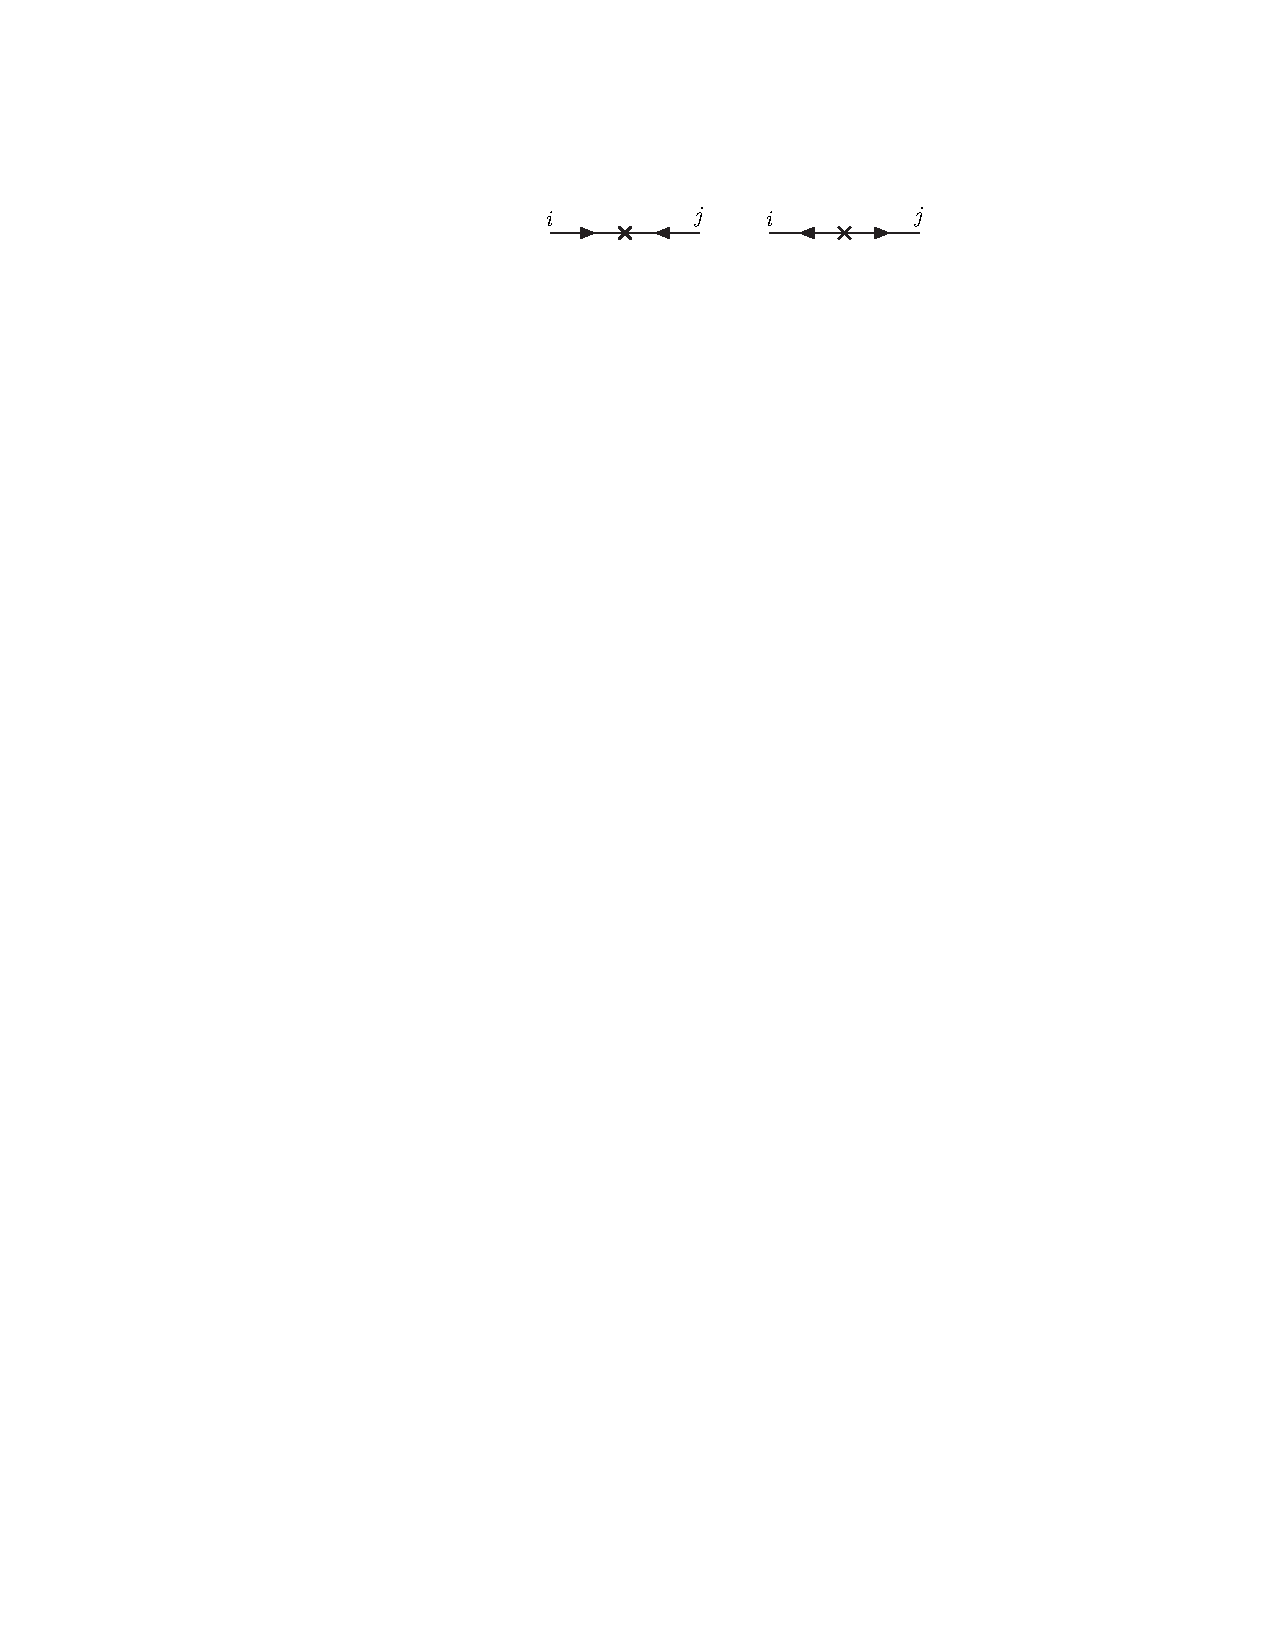
\includegraphics[scale=1.35]{fermion_mass_terms}}
	\hspace{1cm}
	\subfloat[Sfermion mass terms.  Reprinted from Fig. 3.2(e) of ref. \cite{SUSY_primer}.]{\label{fig:sfermion_mass_term}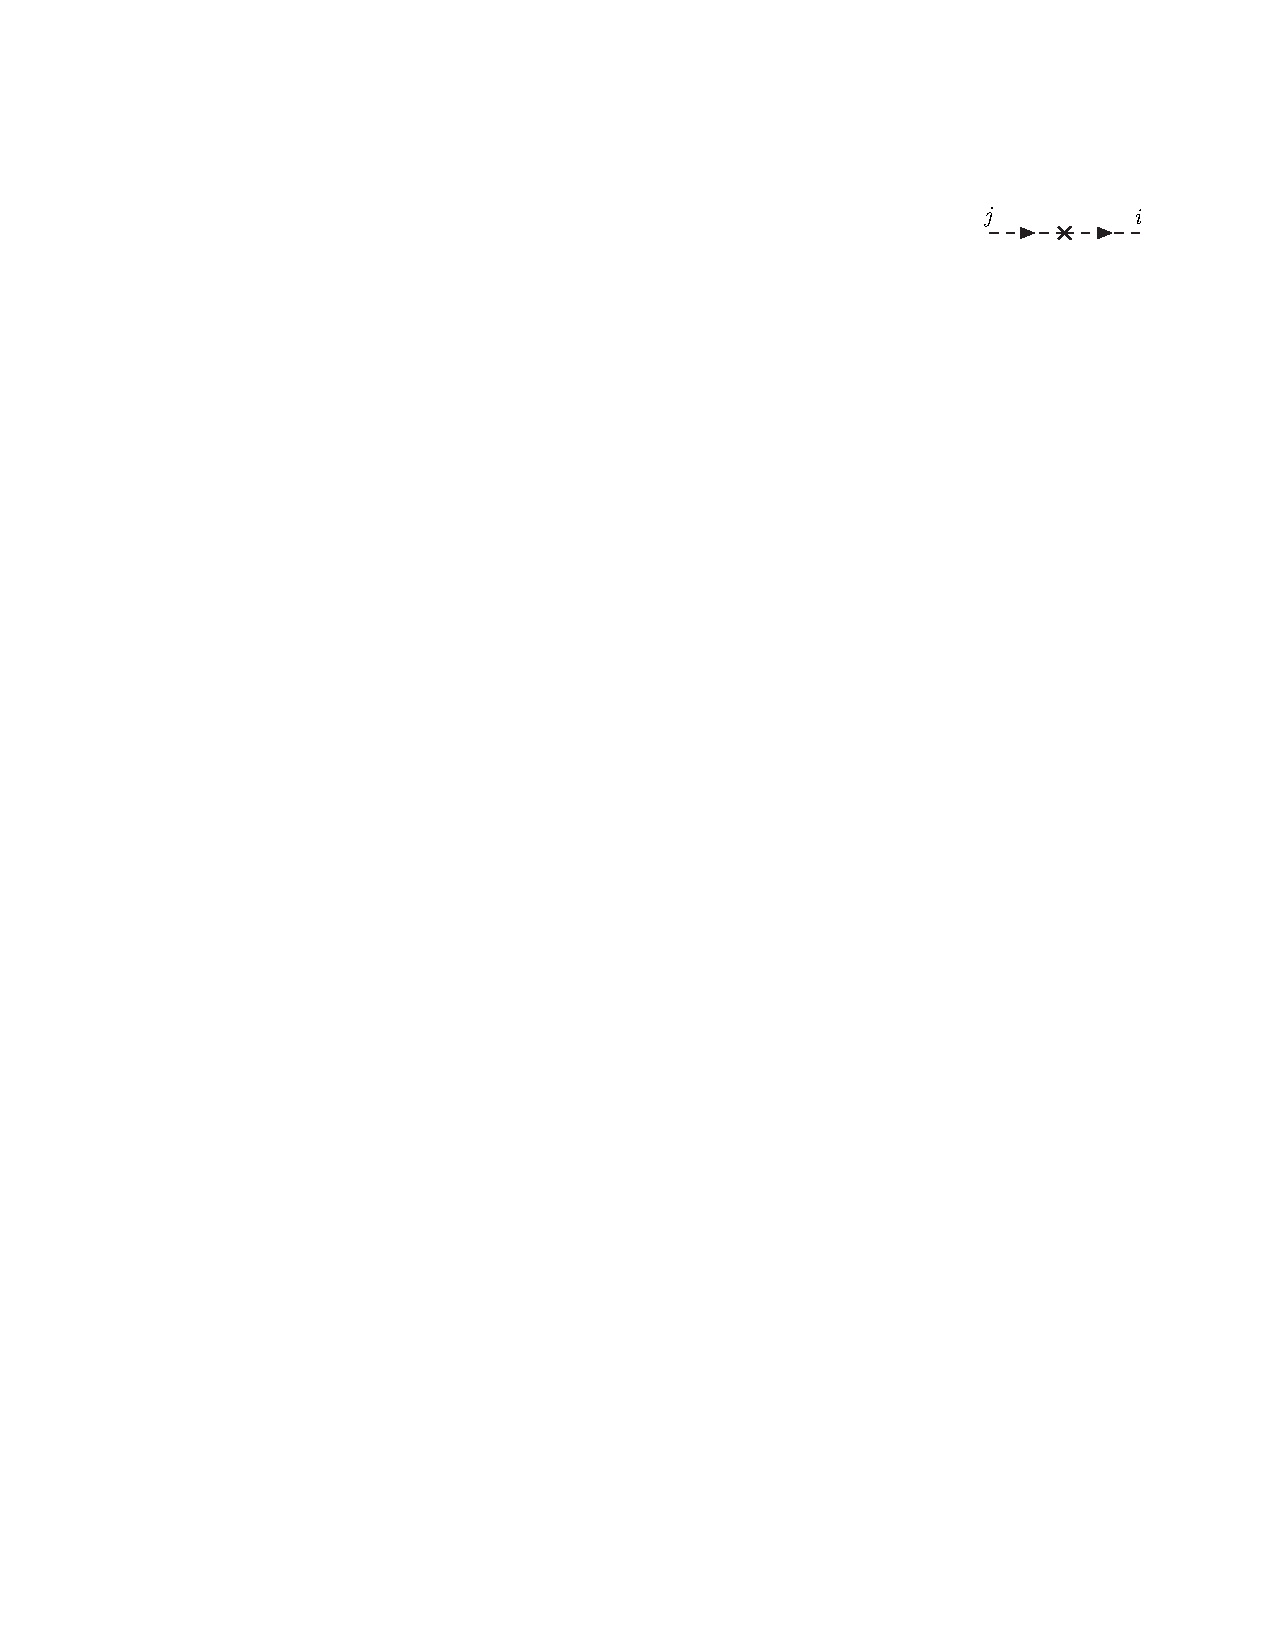
\includegraphics[scale=1.35]{sfermion_mass_term}}
	\\
	\subfloat[$A\phi\phi$ vertex.  Reprinted from Fig. 3.3(e) of ref. \cite{SUSY_primer}.]{\label{fig:Aphiphi_vertex}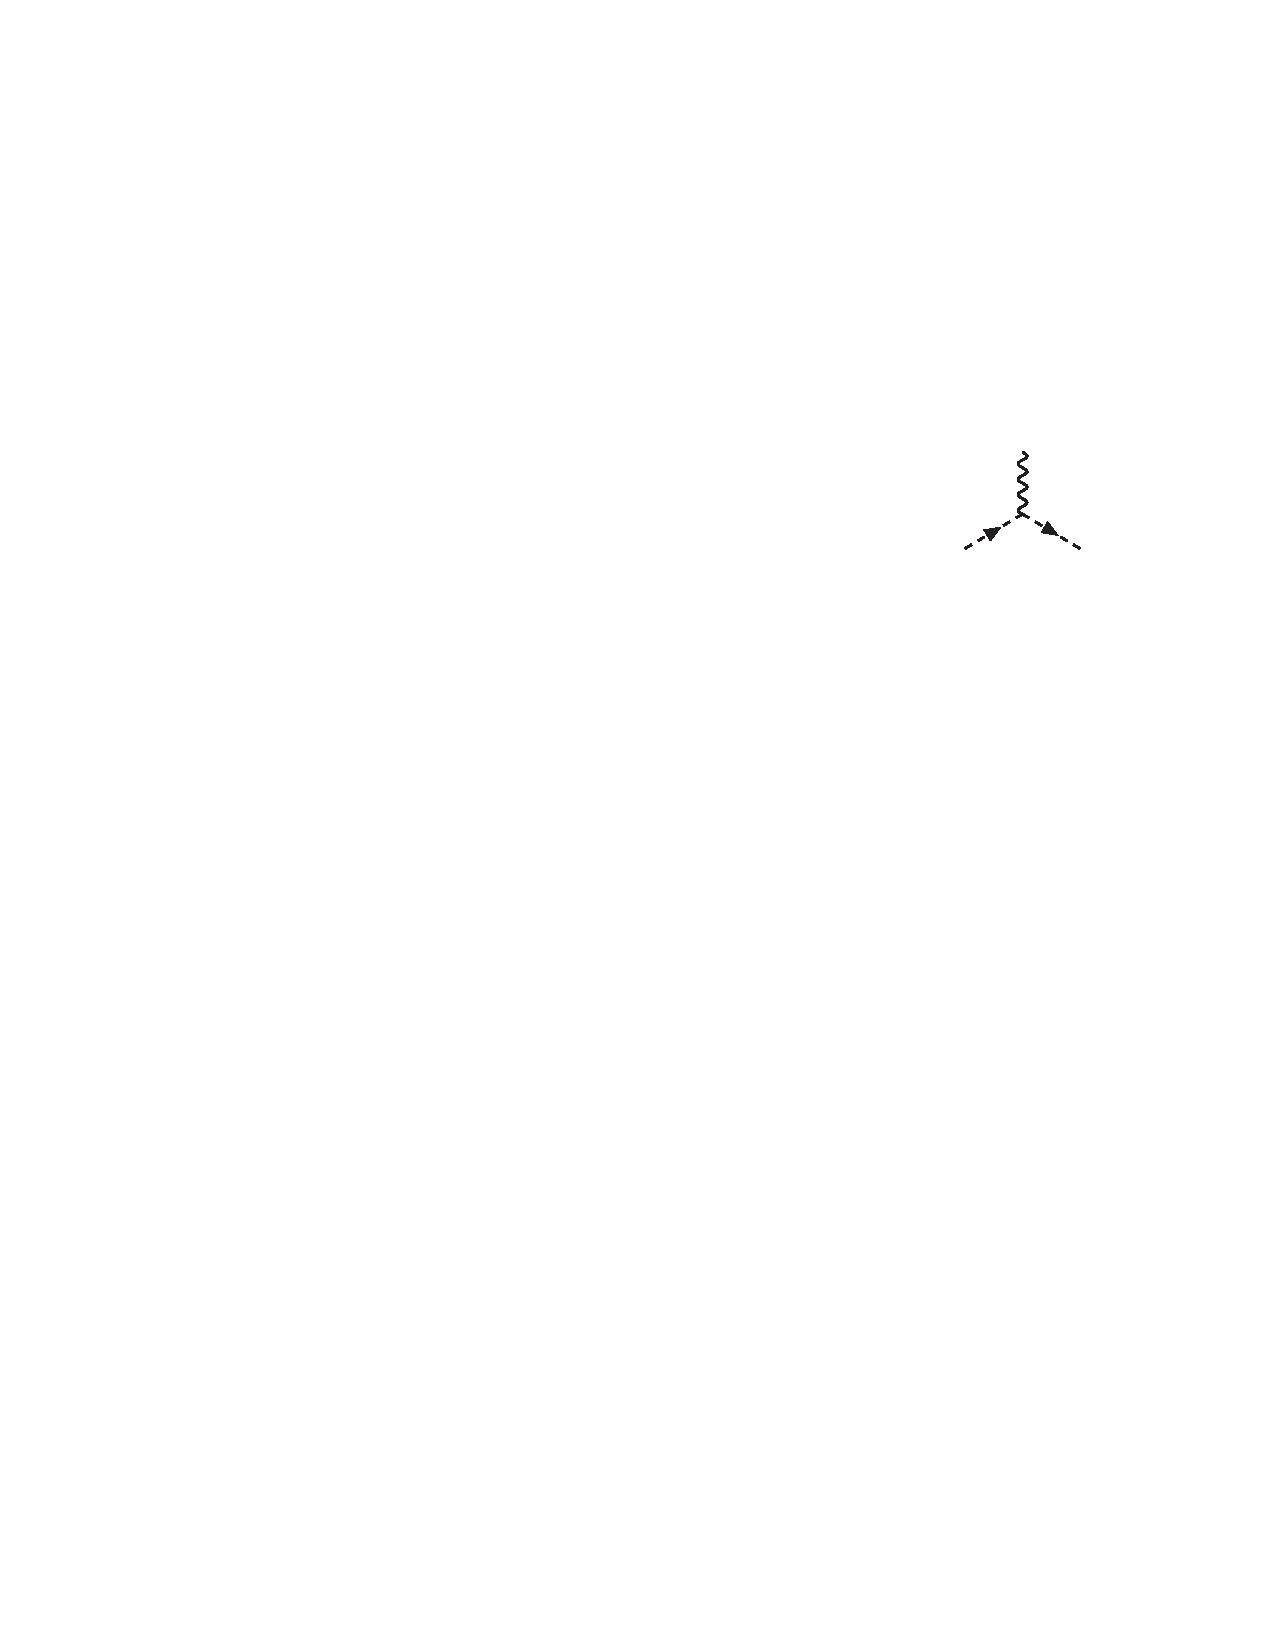
\includegraphics[scale=1.8]{Aphiphi_vertex}}
	\hspace{1cm}
	\subfloat[$A\psi\psi$ vertex.  Reprinted from Fig. 3.3(f) of ref. \cite{SUSY_primer}.]{\label{fig:Apsipsi_vertex}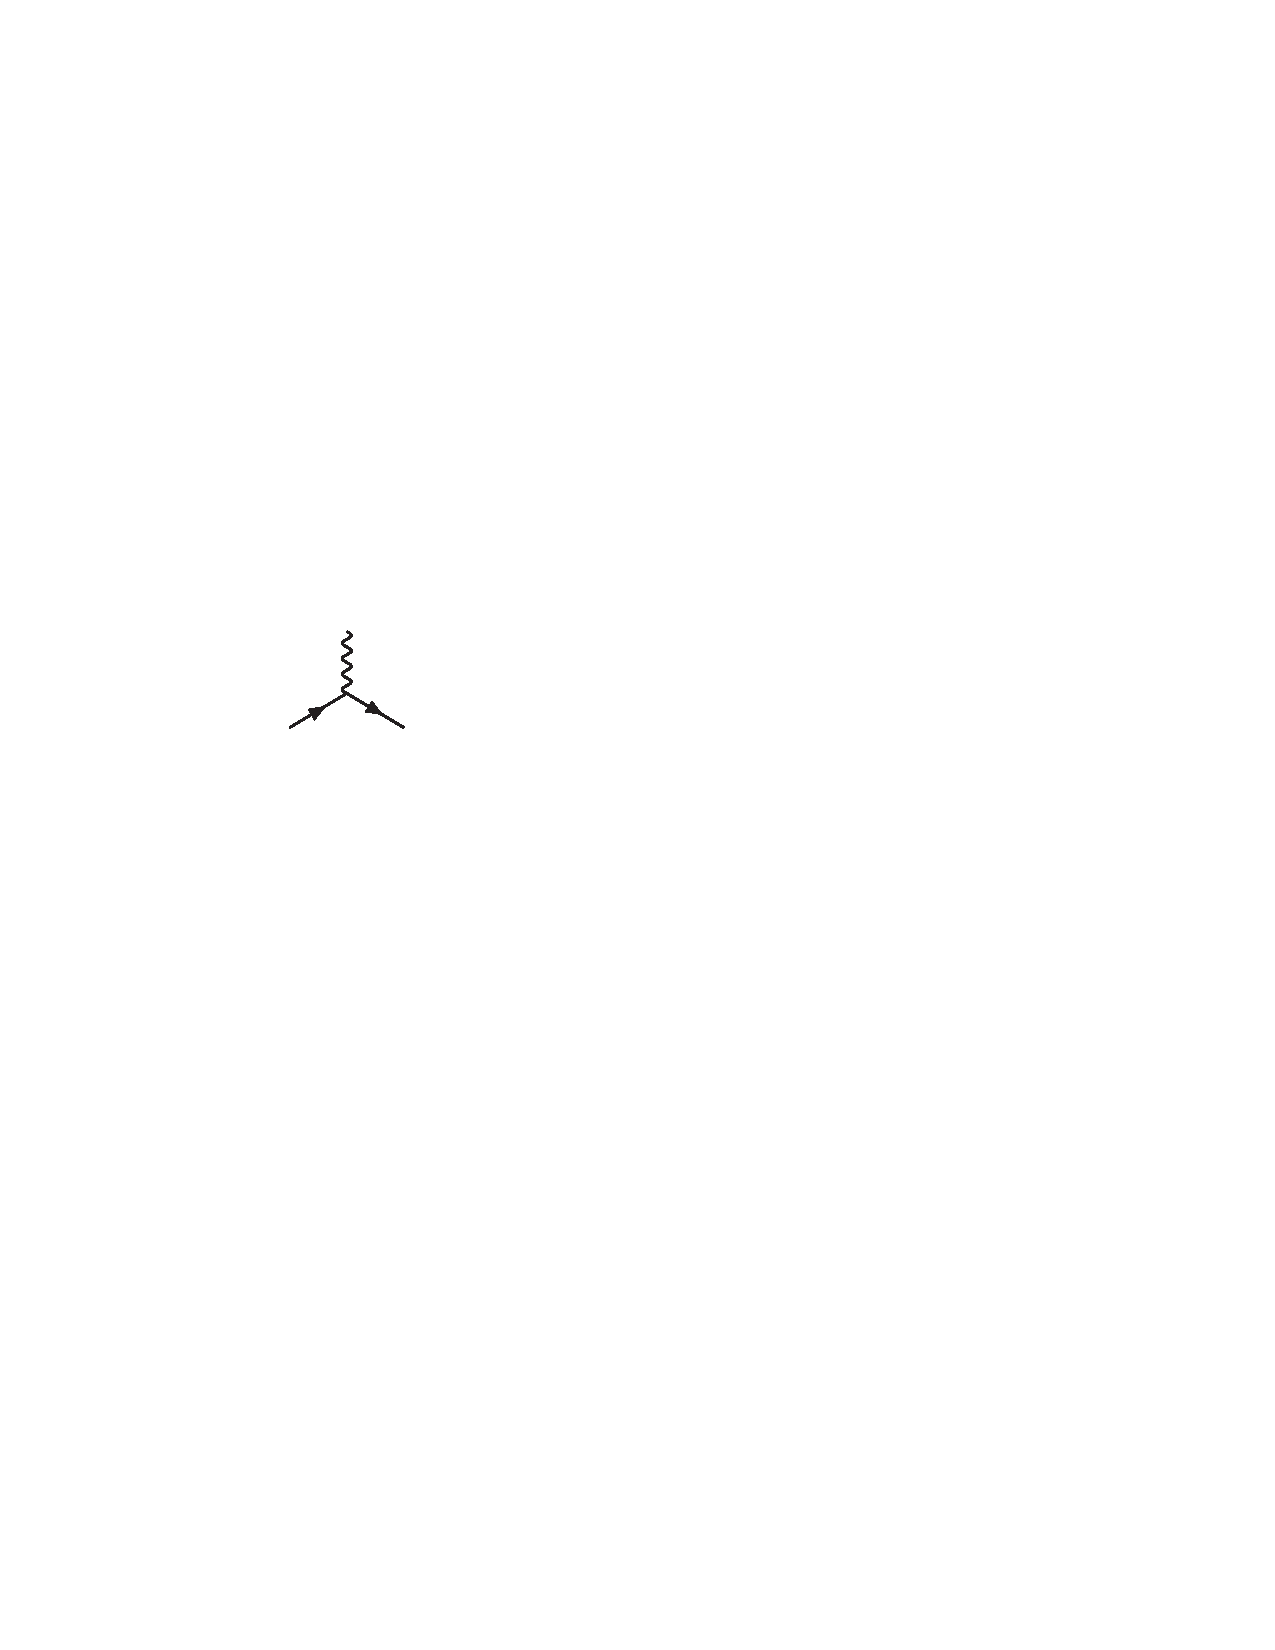
\includegraphics[scale=1.8]{Apsipsi_vertex}}
	\hspace{1cm}
	\subfloat[$A\lambda\lambda$ vertex.  Reprinted from Fig. 3.3(c) of ref. \cite{SUSY_primer}.]{\label{fig:Alambdalambda_vertex}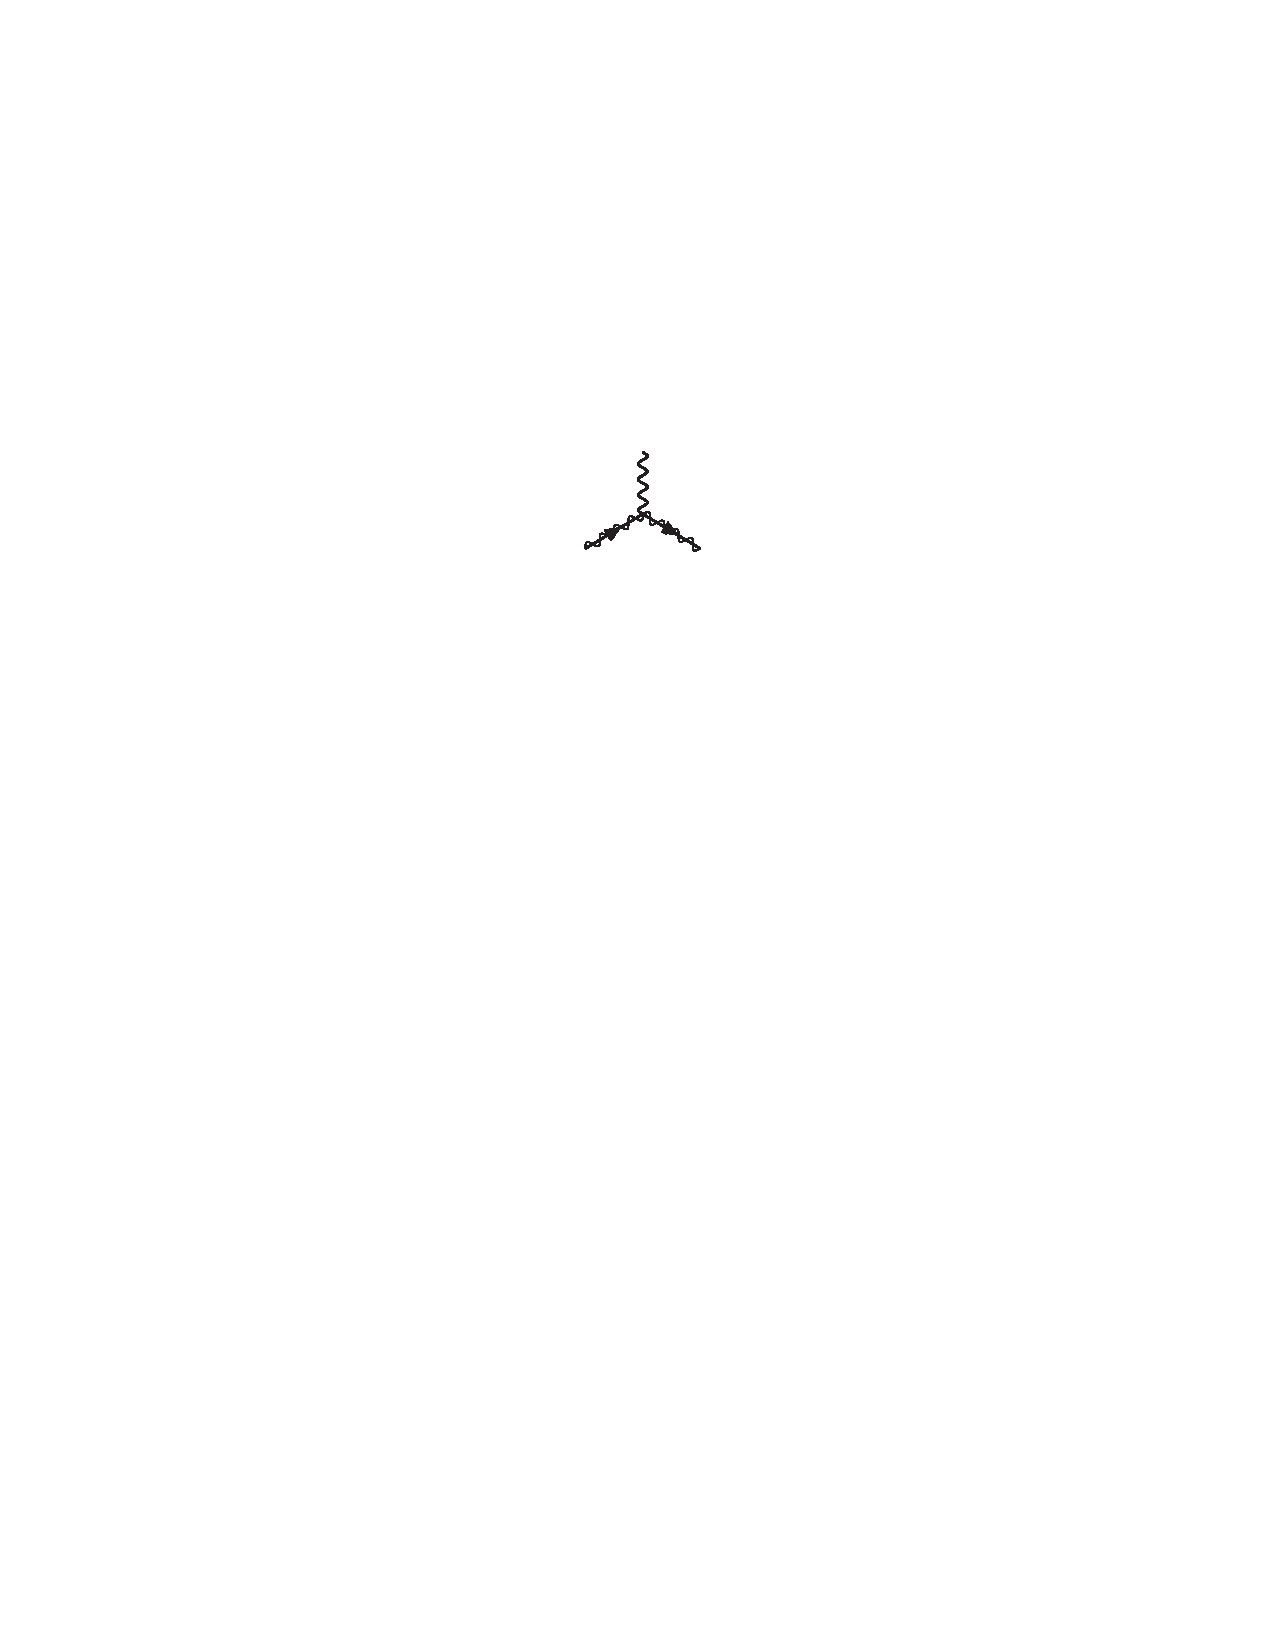
\includegraphics[scale=1.8]{Alambdalambda_vertex}}
	\\
	\subfloat[Triple gauge boson vertex.  Reprinted from Fig. 3.3(b) of ref. \cite{SUSY_primer}.]{\label{fig:triple_gauge_boson_vertex}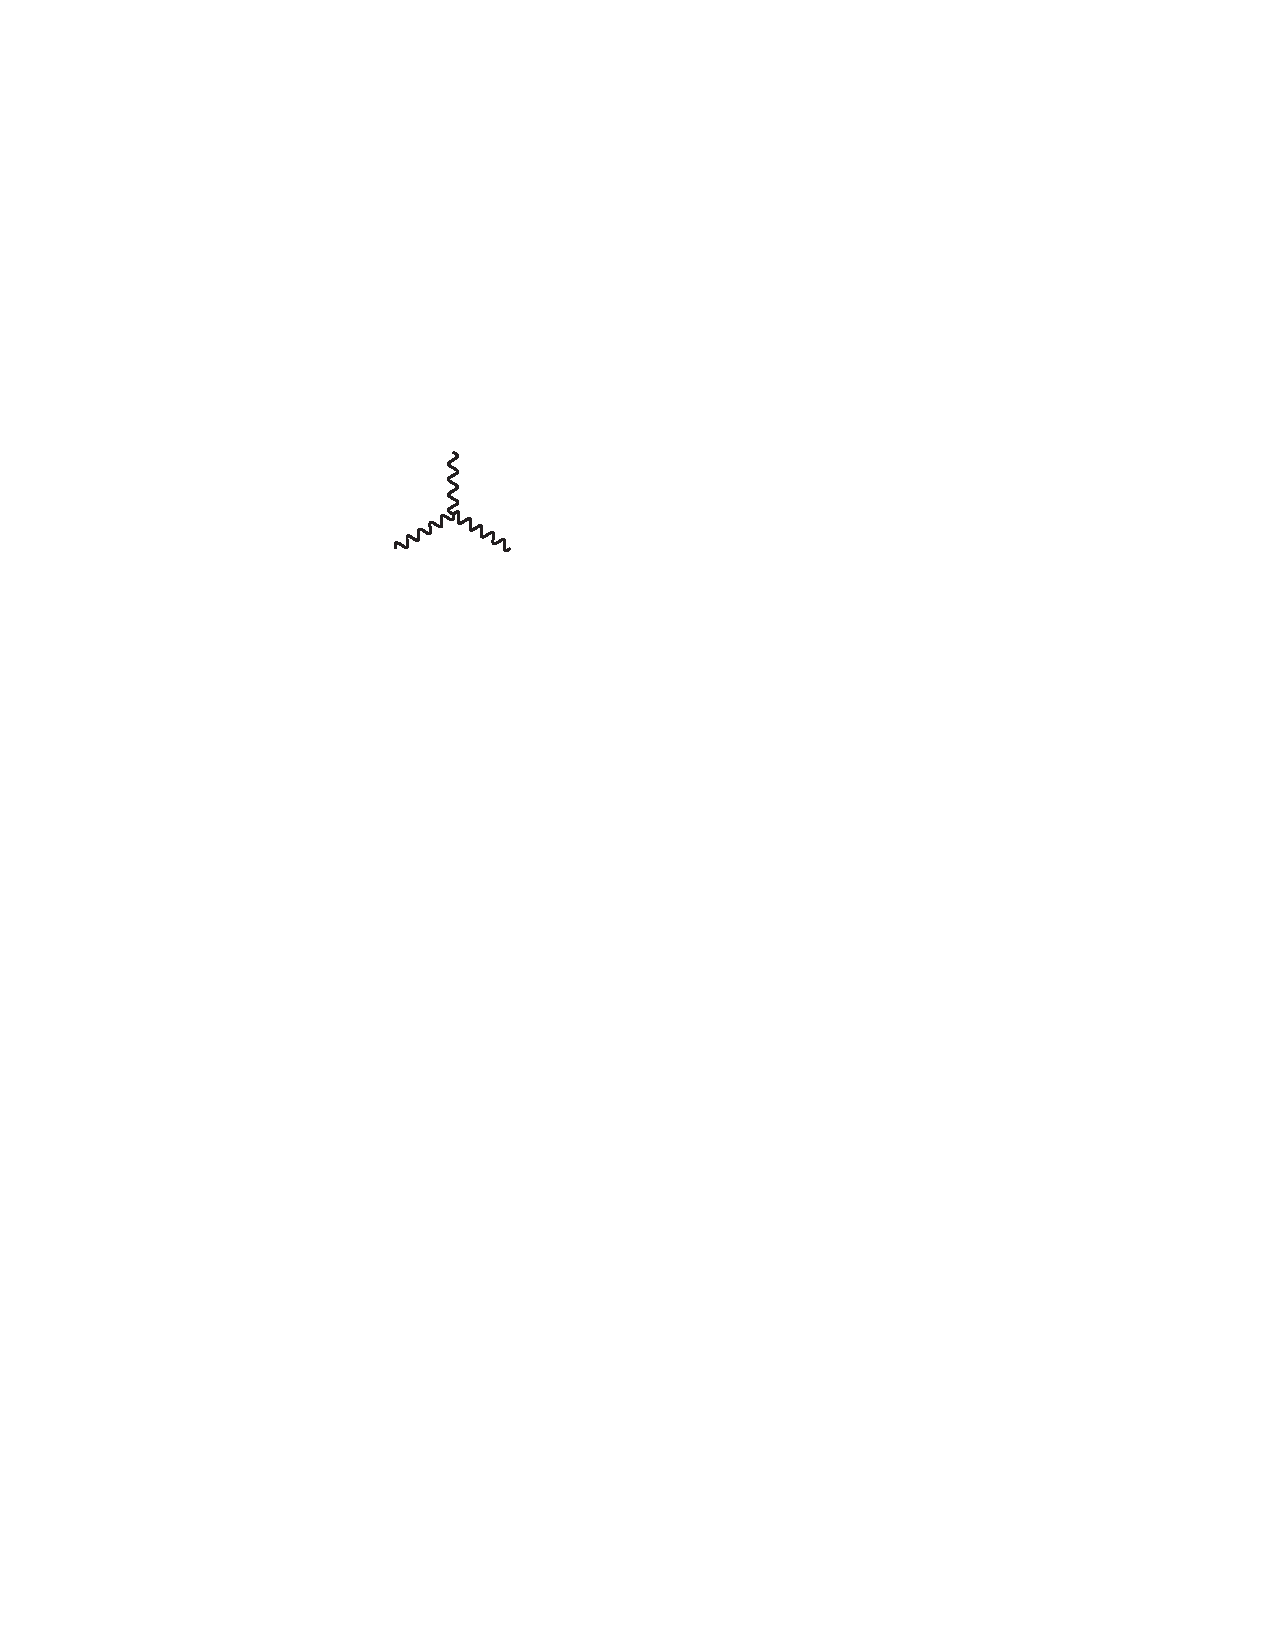
\includegraphics[scale=1.62]{triple_gauge_boson_vertex}}
	\hspace{1cm}
	\subfloat[Triple sfermion vertices.  Reprinted from Figs. 3.2(a) and 3.2(b) of ref. \cite{SUSY_primer}.]{\label{fig:triple_sfermion_vertices}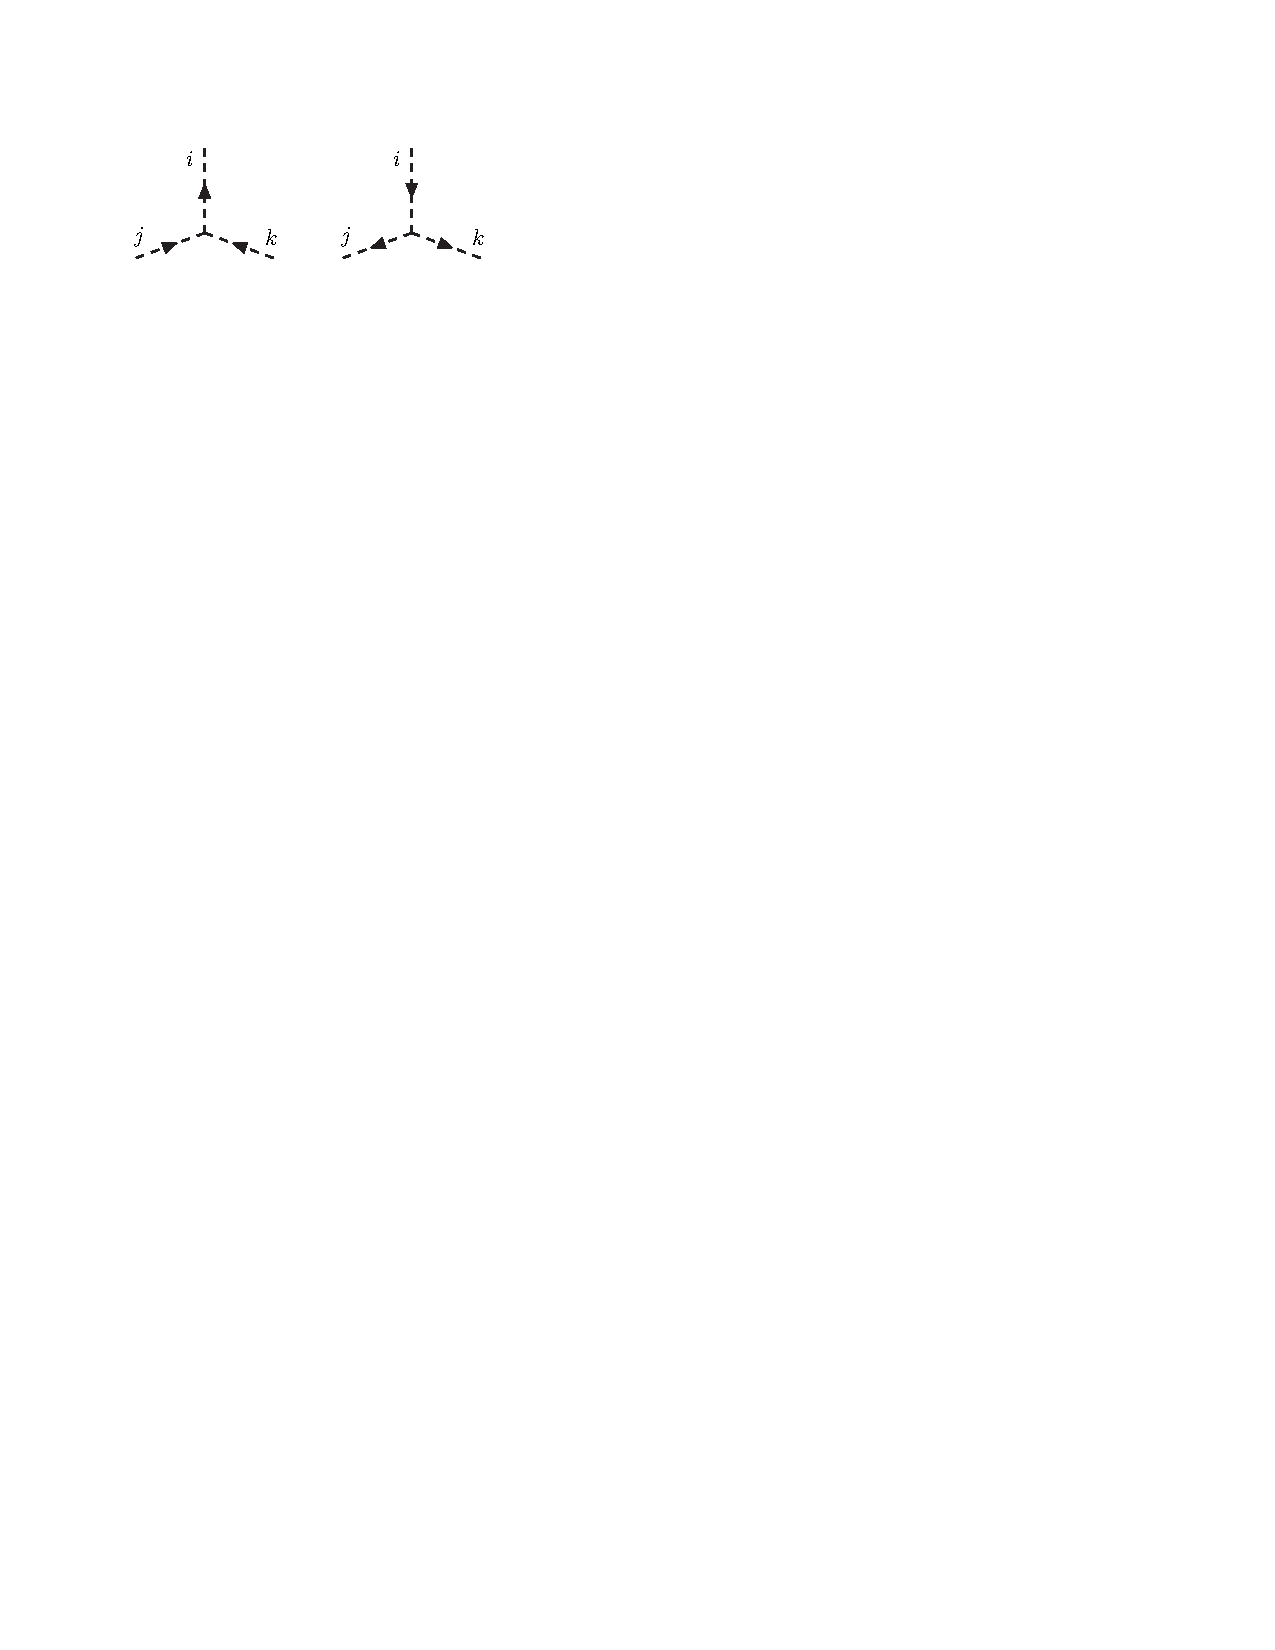
\includegraphics[scale=1.62]{triple_sfermion_vertices}}
	\\
	\subfloat[Cubic couplings in which the fermion radiates a sfermion.  Reprinted from Figs. 3.1(a) and 3.1(b) of ref. \cite{SUSY_primer}.]{\label{fig:phipsipsi_vertices}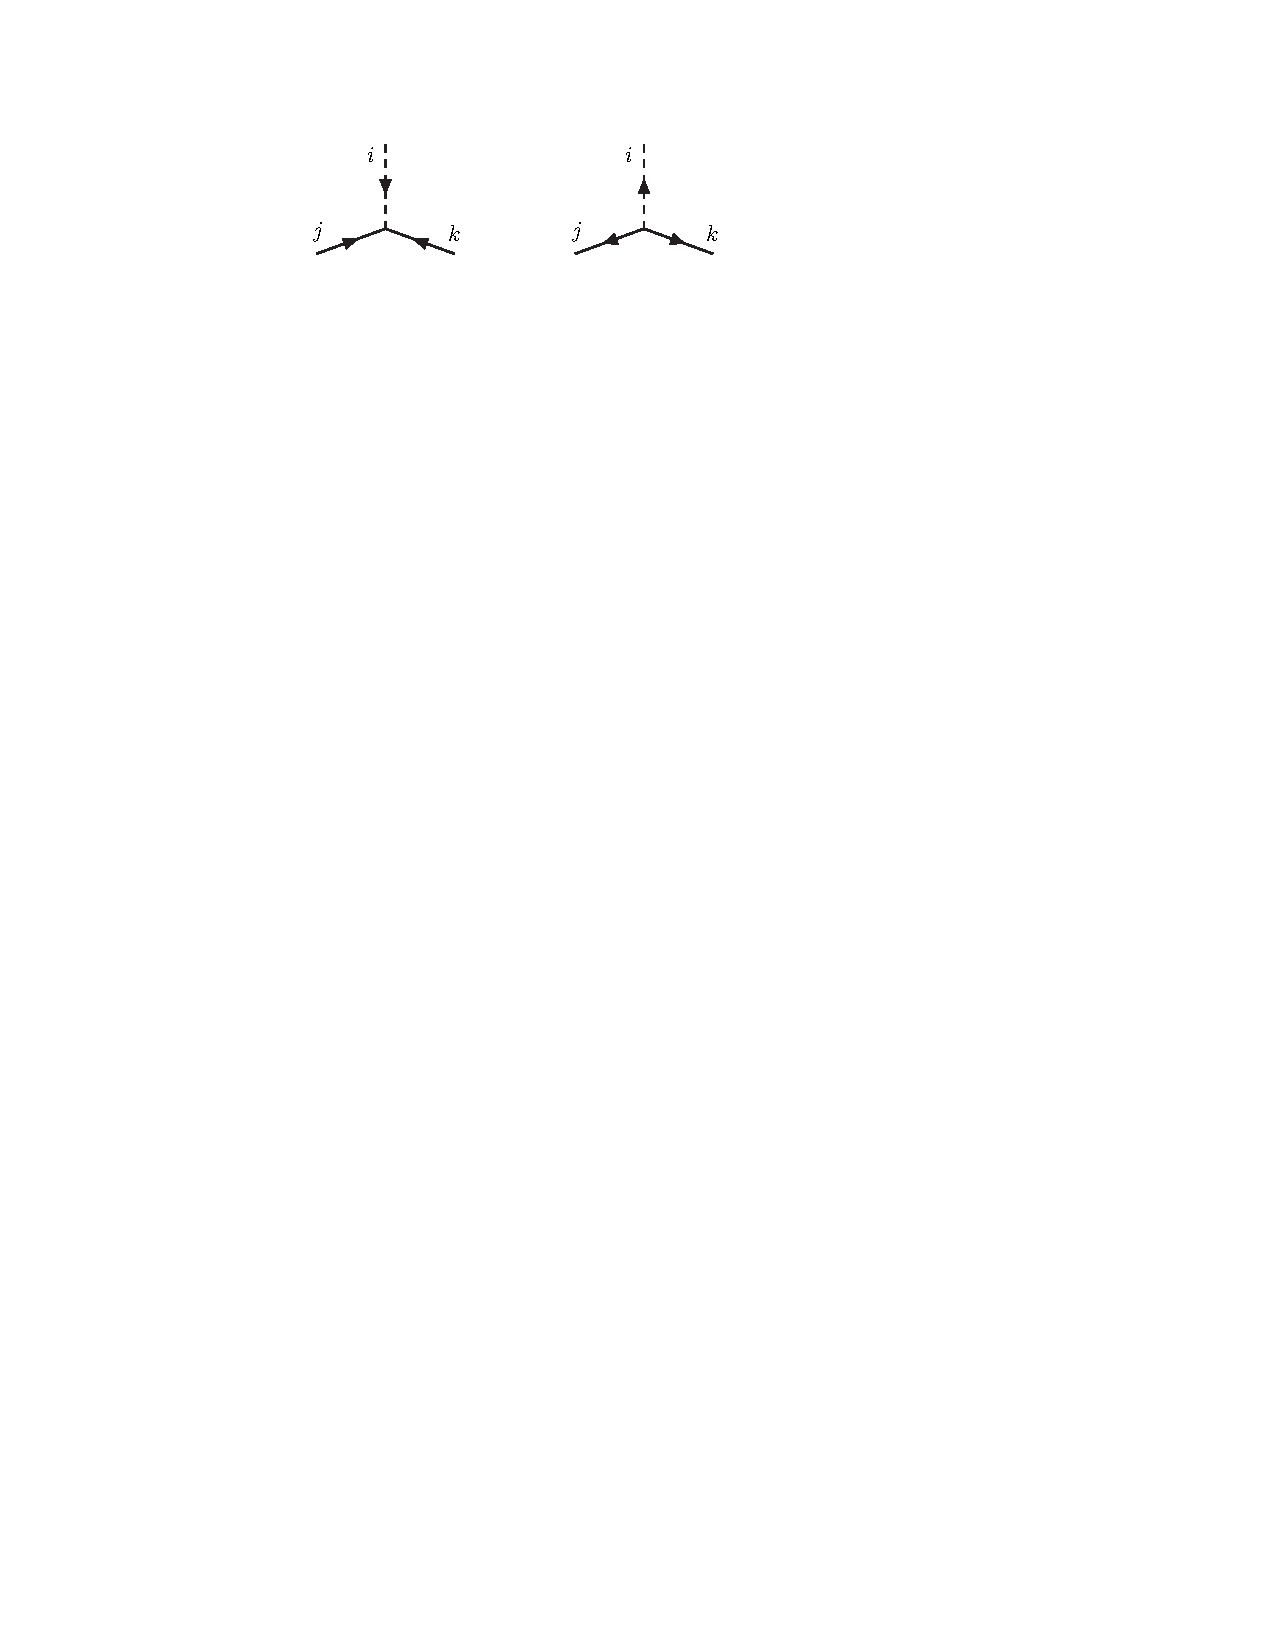
\includegraphics[scale=1.07]{phipsipsi_vertices}}
	\hspace{1cm}
	\subfloat[Sfermion-fermion-gaugino vertices.  Reprinted from Figs. 3.3(g) and 3.3(h) of ref. \cite{SUSY_primer}.]{\label{fig:phipsilambda_vertices}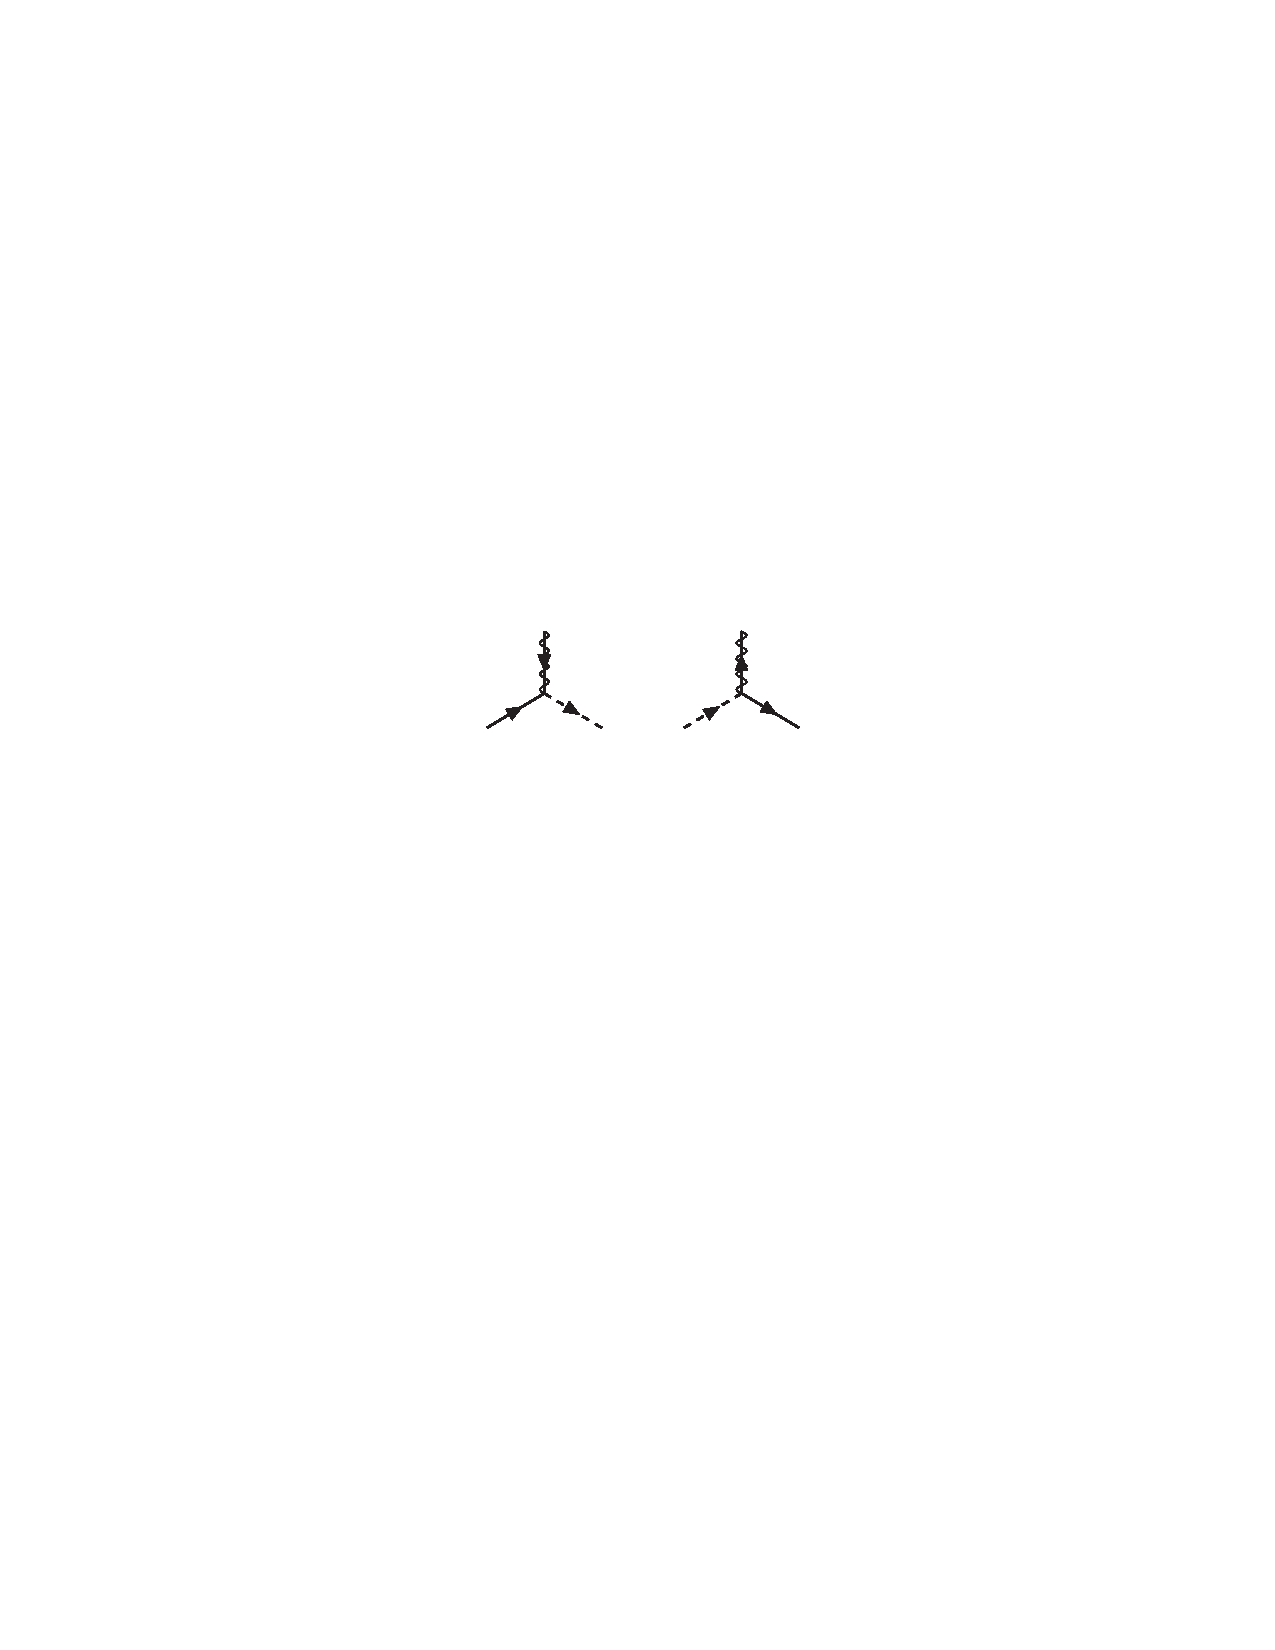
\includegraphics[scale=1.07]{phipsilambda_vertices}}
	\\
	\subfloat[$AA\phi\phi$ vertex.  Reprinted from Fig. 3.3(d) of ref. \cite{SUSY_primer}.]{\label{fig:AAphiphi_vertex}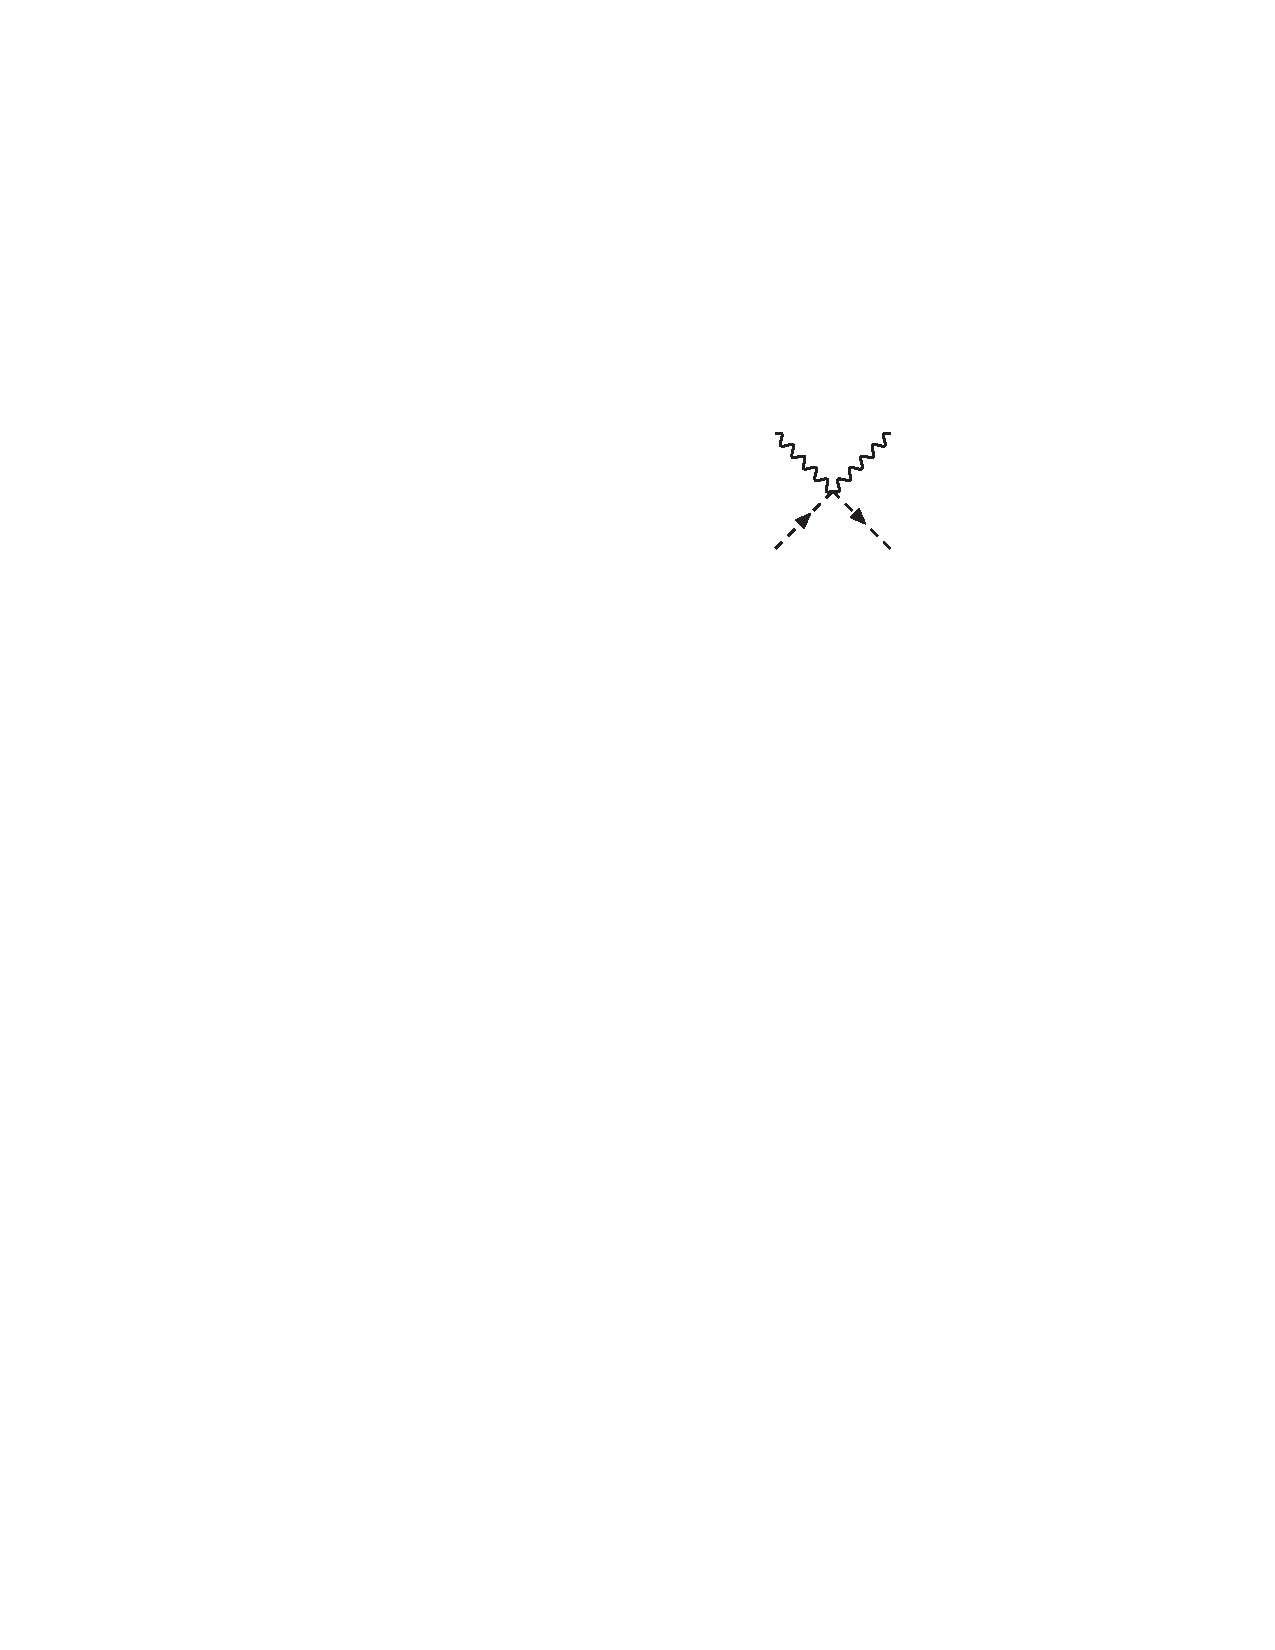
\includegraphics[scale=1.22]{AAphiphi_vertex}}
	\hspace{1cm}
	\subfloat[Quadruple gauge boson vertex.  Reprinted from Fig. 3.3(a) of ref. \cite{SUSY_primer}.]{\label{fig:quadruple_gauge_boson_vertex}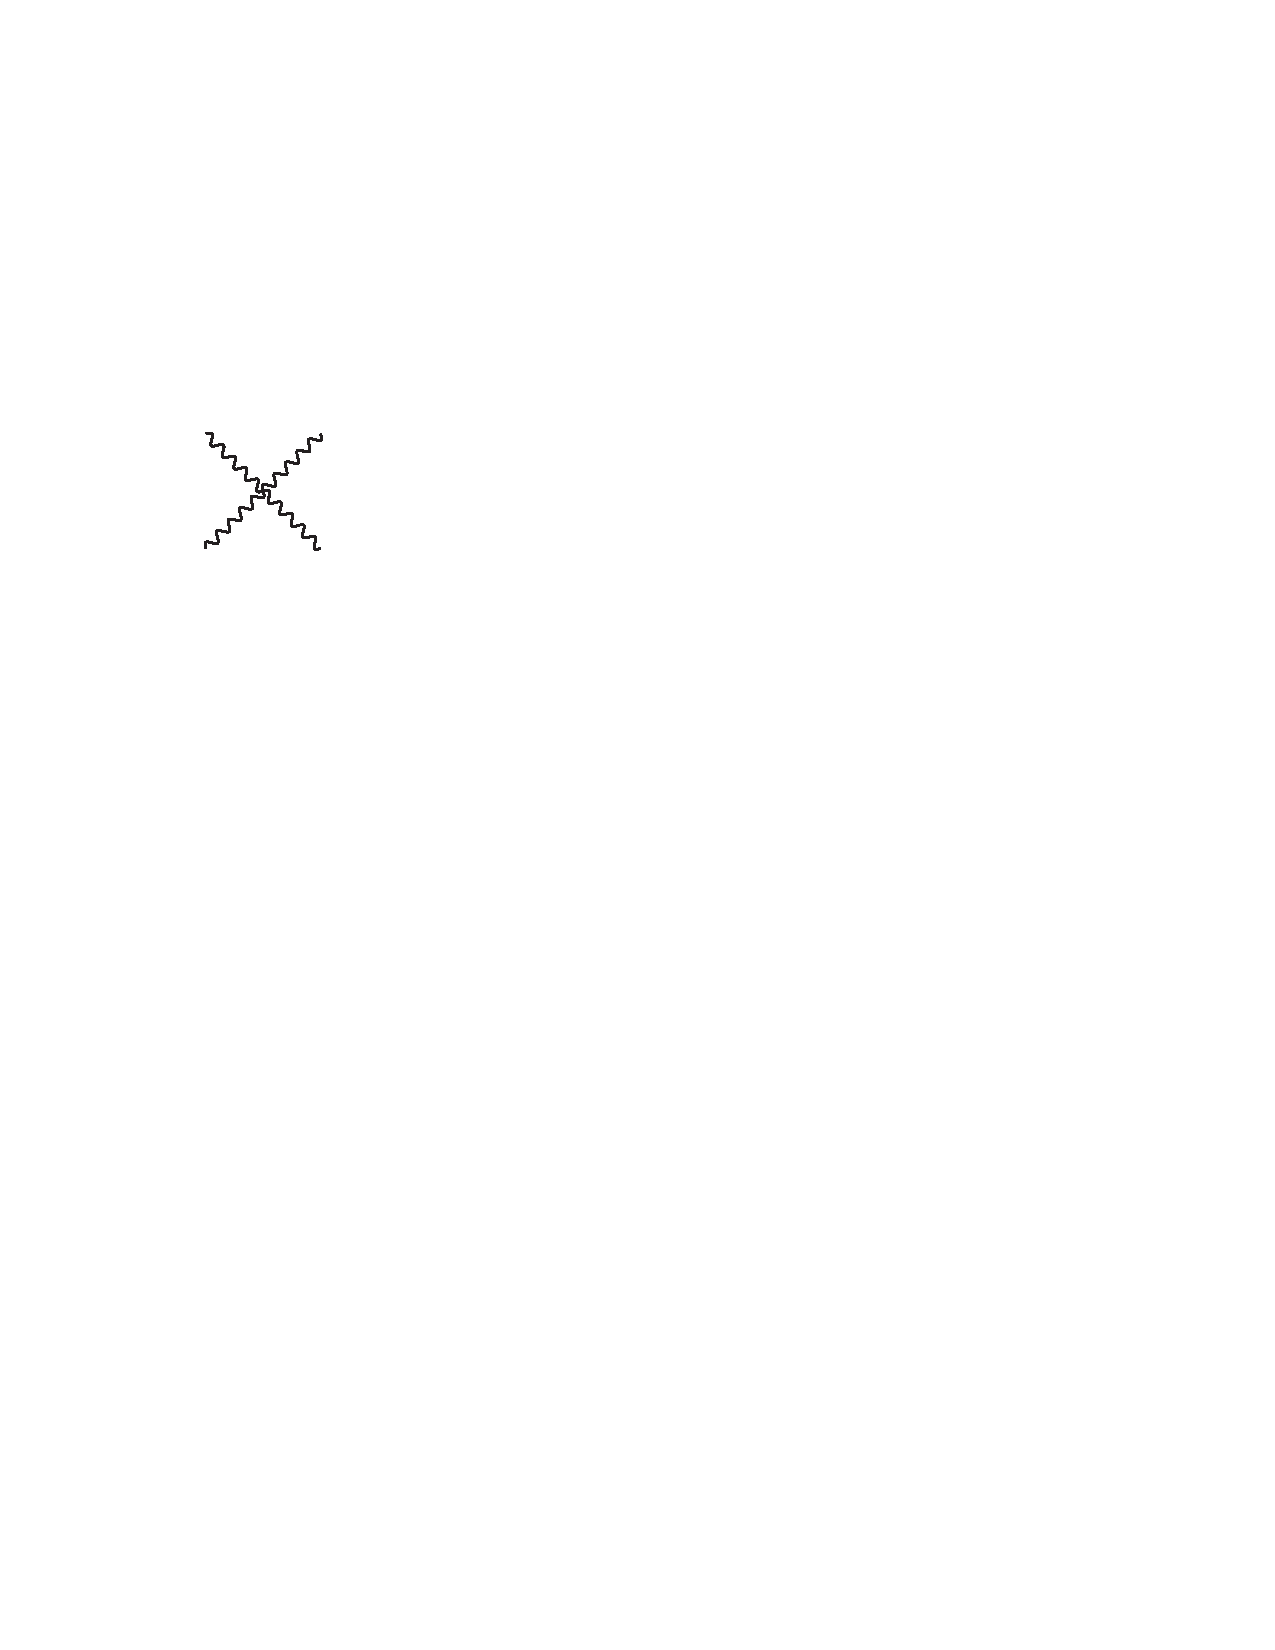
\includegraphics[scale=1.22]{quadruple_gauge_boson_vertex}}
	\hspace{1cm}
	\subfloat[Non-gauge $\phi^{4}$ vertex.  Reprinted from Fig. 3.1(c) of ref. \cite{SUSY_primer}.]{\label{fig:non-gauge_phi4_vertex}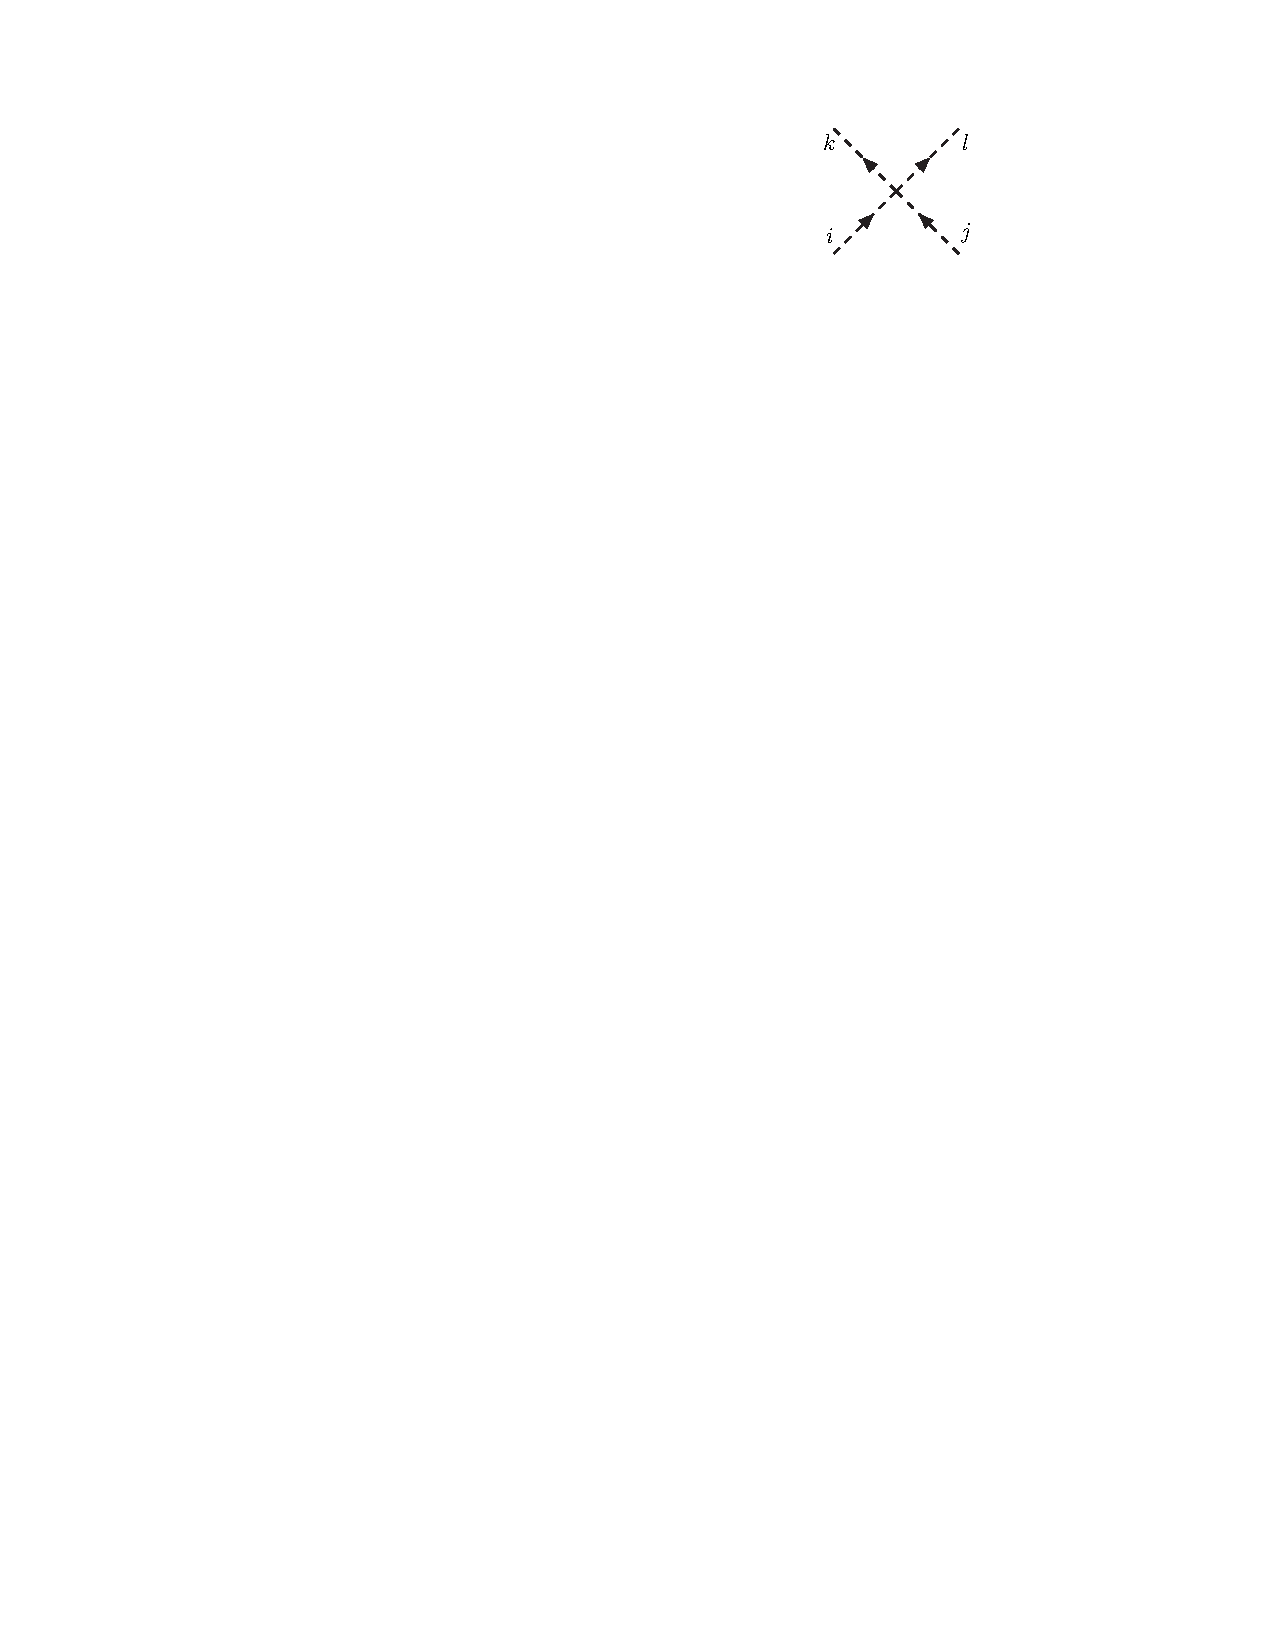
\includegraphics[scale=1.22]{non-gauge_phi4_vertex}}
	\hspace{1cm}
	\subfloat[Gauge $\phi^{4}$ vertex.  Reprinted from Fig. 3.3(i) of ref. \cite{SUSY_primer}.]{\label{fig:gauge_phi4_vertex}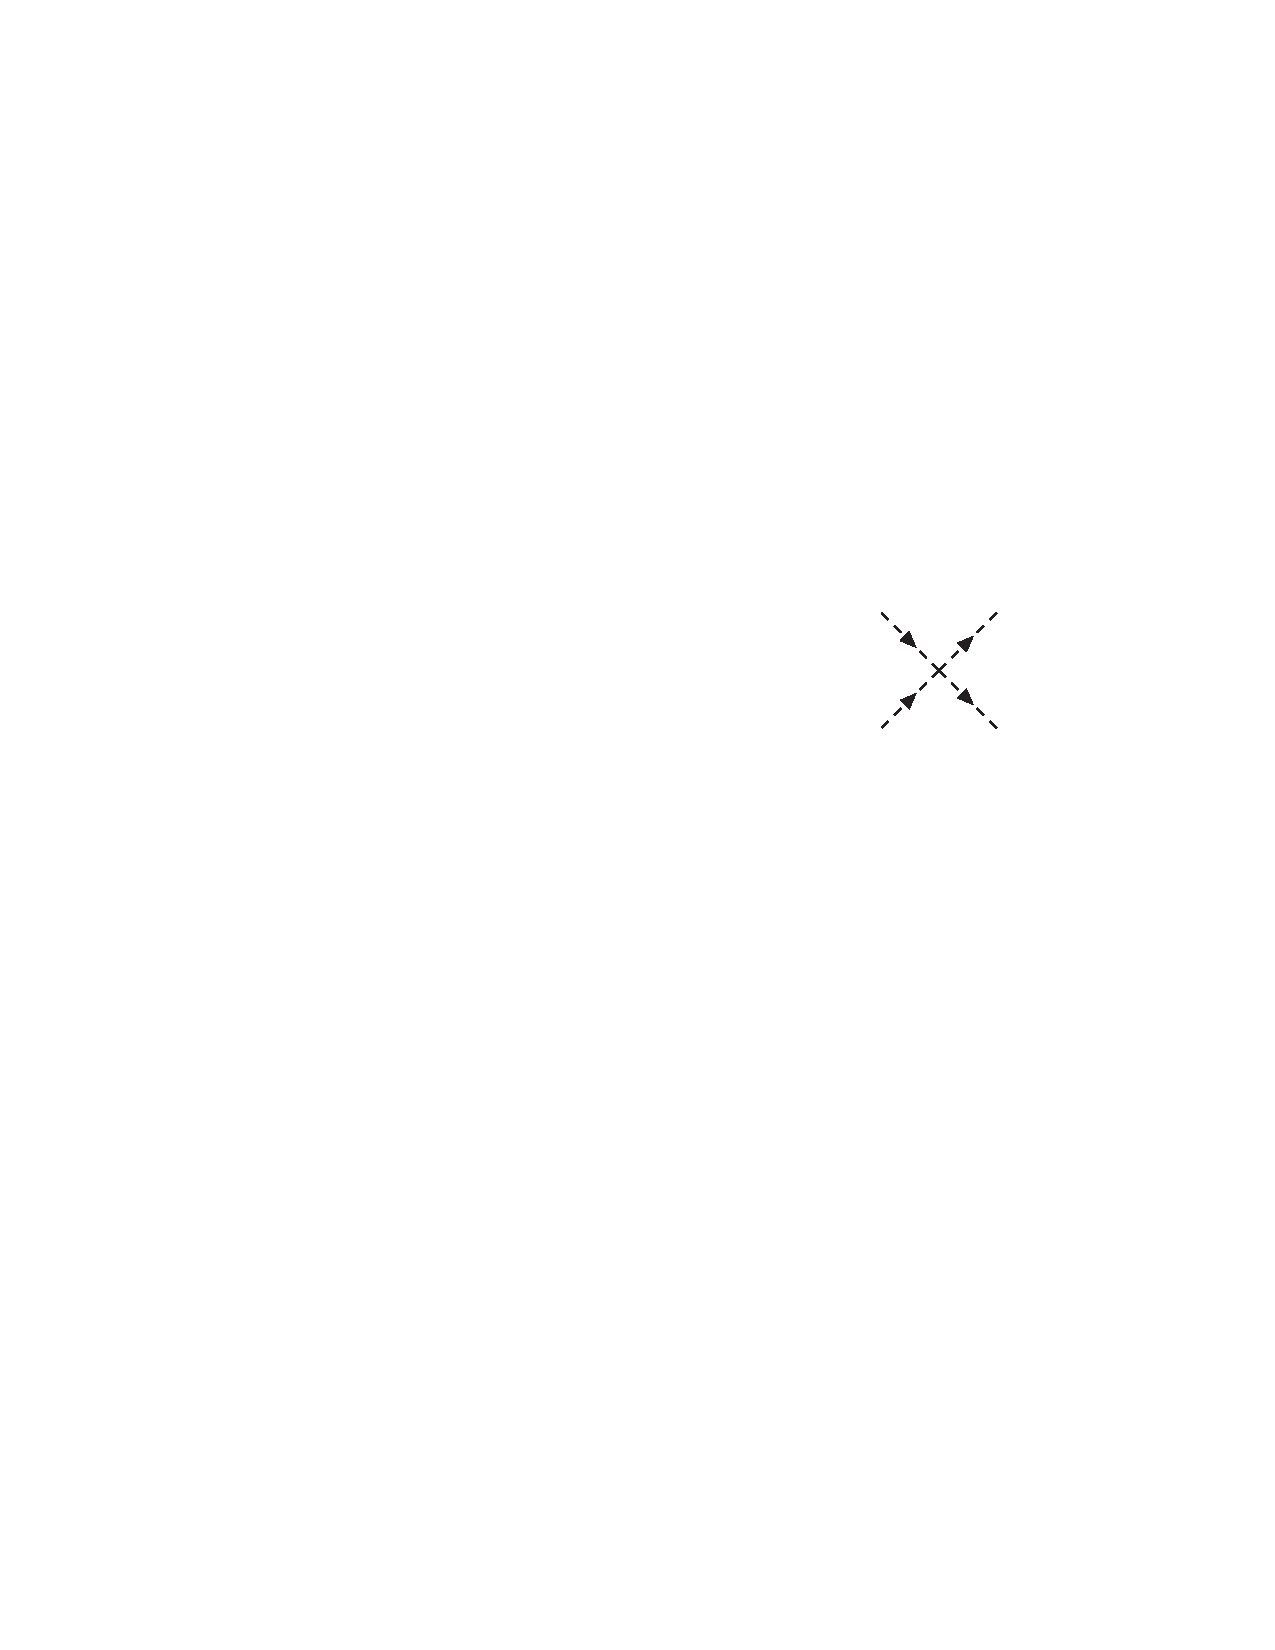
\includegraphics[scale=1.22]{gauge_phi4_vertex}}
	\caption{Interactions in the unbroken SUSY Lagrangian.}
	\label{fig:unbroken_SUSY_interactions}
\end{figure}

\section{Soft SUSY Breaking}
\label{sec:Soft SUSY Breaking}

Since quadratic divergences in sfermion masses vanish to all orders in perturbation theory in plain unbroken SUSY \cite{SUSY_primer} due to the presence of gauge and Yukawa interactions with the necessary relationships between coupling constants, it is desirable that the terms that break SUSY not disturb this property.  In addition, SUSY should be broken spontaneously, as electroweak symmetry is broken in the Standard Model, so that it is only made manifest at high energies.  To satisfy these constraints, SUSY-breaking terms are simply added to the unbroken SUSY Lagrangian in Eq.~\ref{eq:L_final} such that $\mathcal{L}_{\mathrm{total}} = \mathcal{L}_{\mathrm{unbroken}} + \mathcal{L}_{\mathrm{breaking}}$.  The coefficients of terms in $\mathcal{L}_{\mathrm{breaking}}$ must have positive mass dimension in order not to contribute quadratically divergent loop corrections to the scalar masses (like the Higgs mass).\footnote{This point can be argued via dimensional analysis.  Radiative corrections take the form $\Delta m_{S}^{2}$, where $m_{S}$ is the mass of the scalar particle in question.  The dimensions of $\Delta m_{S}^{2}$ are $\mbox{mass}^{2}$.  $\Delta m_{S}^{2}$ is proportional to some coupling constant or mass coefficient $k$ multiplied by a function of $\Lambda_{\mathrm{UV}}$, the high energy cutoff scale.  The function of $\Lambda_{\mathrm{UV}}$ is determined by a loop integral, and thus typically takes the form $\Lambda_{\mathrm{UV}}^{2}$ (quadratically divergent) or $\ln\frac{\Lambda_{\mathrm{UV}}}{m_{\mathrm{low}}}$ (logarithmically divergent, where $m_{\mathrm{low}}$ is some other lower-mass scale in the problem).  Now, if $k$ already contributes at least one power of mass to $\Delta m_{S}^{2}$, then the high-energy behavior---the function of $\Lambda_{\mathrm{UV}}$---can only contribute at most one power of the dimensionful parameter $\Lambda_{\mathrm{UV}}$.  However, there are typically no loop integrals that diverge linearly in $\Lambda_{\mathrm{UV}}$, so by forcing $k$ to have positive mass dimension, the form of the radiative corrections contributed by SUSY-breaking terms is limited to $\Delta m_{S}^{2} \sim m_{\mathrm{low}}^{2}\ln\frac{\Lambda_{\mathrm{UV}}}{m_{\mathrm{low}}}$.  In effect, the possibility of dangerous corrections proportional to $\Lambda_{\mathrm{UV}}^{2}$ is excluded by dimensional analysis if the requirement that $k$ contribute at least one power of mass is enforced.}  This form of SUSY breaking is called \textit{soft}, and all coefficients of soft SUSY breaking terms are expected to be of order $m_{\mathrm{soft}}$ or $m_{\mathrm{soft}}^{2}$.

Soft SUSY breaking terms give masses to the sfermions and gauginos and introduce a cubic sfermion vertex.  The soft terms are given by

%why are some family indices in upstairs-downstairs notation and some not?
\begin{eqnarray}
\label{eq:L_soft}
\mathcal{L}_{\mathrm{soft}} &=& -\frac{1}{2}(M_{3}\widetilde{g}^{a}\widetilde{g}^{a}\mbox{ + }M_{2}\widetilde{W}^{a}\widetilde{W}^{a}\mbox{ + }M_{1}\widetilde{B}\widetilde{B}\mbox{ + h.c.})\nonumber \\
&&-\mbox{ }(a_{u}^{ij}\widetilde{u}_{Ri}^{*}\widetilde{Q}_{j}H_{u} - a_{d}^{ij}\widetilde{d}_{Ri}^{*}\widetilde{Q}_{j}H_{d} - a_{e}^{ij}\widetilde{e}_{Ri}^{*}\widetilde{L}_{j}H_{d}\mbox{ + h.c.})\nonumber \\
&&-\mbox{ }m_{\widetilde{Q}ij}^{2}\widetilde{Q}_{i}^{\dag}\widetilde{Q}_{j}\mbox{ }-\mbox{ }m_{\widetilde{L}ij}^{2}\widetilde{L}_{i}^{\dag}\widetilde{L}_{j}\mbox{ }\nonumber \\
&&-\mbox{ }m_{\widetilde{\overline{u}}ij}^{2}\widetilde{u}_{Ri}\widetilde{u}_{Rj}^{*}\mbox{ }-\mbox{ }m_{\widetilde{\overline{d}}ij}^{2}\widetilde{d}_{Ri}\widetilde{d}_{Rj}^{*}\mbox{ }-\mbox{ }m_{\widetilde{\overline{e}}ij}^{2}\widetilde{e}_{Ri}\widetilde{e}_{Rj}^{*}\mbox{ }\nonumber \\
&&-\mbox{ }m_{H_{u}}^{2}H_{u}^{*}H_{u}\mbox{ }-\mbox{ }m_{H_{d}}^{2}H_{d}^{*}H_{d}\mbox{ }-\mbox{ }(bH_{u}H_{d}\mbox{ + h.c.})
\end{eqnarray}
%first line: Weyl spinor products
%second line: SU(2) 2 x 2 product (just like Weyl spinor product)
%third line: SU(2) 2 x 2-bar product (like a magnitude squared)
%fourth line: 2 x 2 and 2 x 2-bar products
where $a$ runs from 1-8 for $\widetilde{g}^{a}$ and from 1-3 for $\widetilde{W}^{a}$, and $i,j$ run over the three families.  The color indices are not shown.  The first line of Eq.~\ref{eq:L_soft} contains the gaugino mass terms.  The second line contains cubic scalar couplings that contribute to mixing between the left- and right-handed third generation sfermions (it is assumed in the supersymmetric Standard Model that the $a_{u}^{ij}$, $a_{d}^{ij}$, and $a_{e}^{ij}$ are negligible unless $i = j = 3$).  The third and fourth lines of Eq.~\ref{eq:L_soft} contain squark and slepton mass terms, and finally the last line contains the Higgs mass terms.

Many viable models of achieving soft SUSY breaking have been studied over the last 30 years.  For an overview, see Sec. 6 of ref. \cite{SUSY_primer}.  However, this thesis will only cover \textit{gauge-mediated SUSY breaking} (GMSB), because the two-photon search performed is far more sensitive to this model than to other models of SUSY breaking.

\section{Gauge-Mediated SUSY Breaking}
\label{sec:Gauge-Mediated SUSY Breaking}

%how do the messengers interact with the ordinary particles?
%include a diagram of the communication between the sectors?
In gauge-mediated models \cite{GMSB}, ``hidden" fields spontaneously break the supersymmetry of very heavy chiral \textit{messenger} supermultiplets.  There are a number of competing models (see ref. \cite{GMSB}) that explain the precise mechanism of spontaneous SUSY breaking, but fortunately the details of those models mostly decouple from the phenomenology of GMSB.  The messengers then communicate the SUSY breaking to the sparticles via loop diagrams of gauge interaction strength (i.e. via vertices like those shown in Figs.~\subref*{fig:Aphiphi_vertex},~\subref*{fig:Apsipsi_vertex},~\subref*{fig:phipsilambda_vertices},~\subref*{fig:AAphiphi_vertex}, and~\subref*{fig:gauge_phi4_vertex}, which are proportional to the SM gauge couplings constants).  Feynman diagrams corresponding to gaugino and sfermion mass terms are shown in Figure~\ref{fig:gaugino_sfermion_GMSB_mass_terms}.

\begin{figure}
	\centering
	\subfloat[Sfermion mass terms.  Heavy dashed lines denote messenger sfermions; solid lines denote messenger fermions.  Reprinted from Fig. 6.4 of ref. \cite{SUSY_primer}.]{\label{fig:sfermion_GMSB_mass_terms}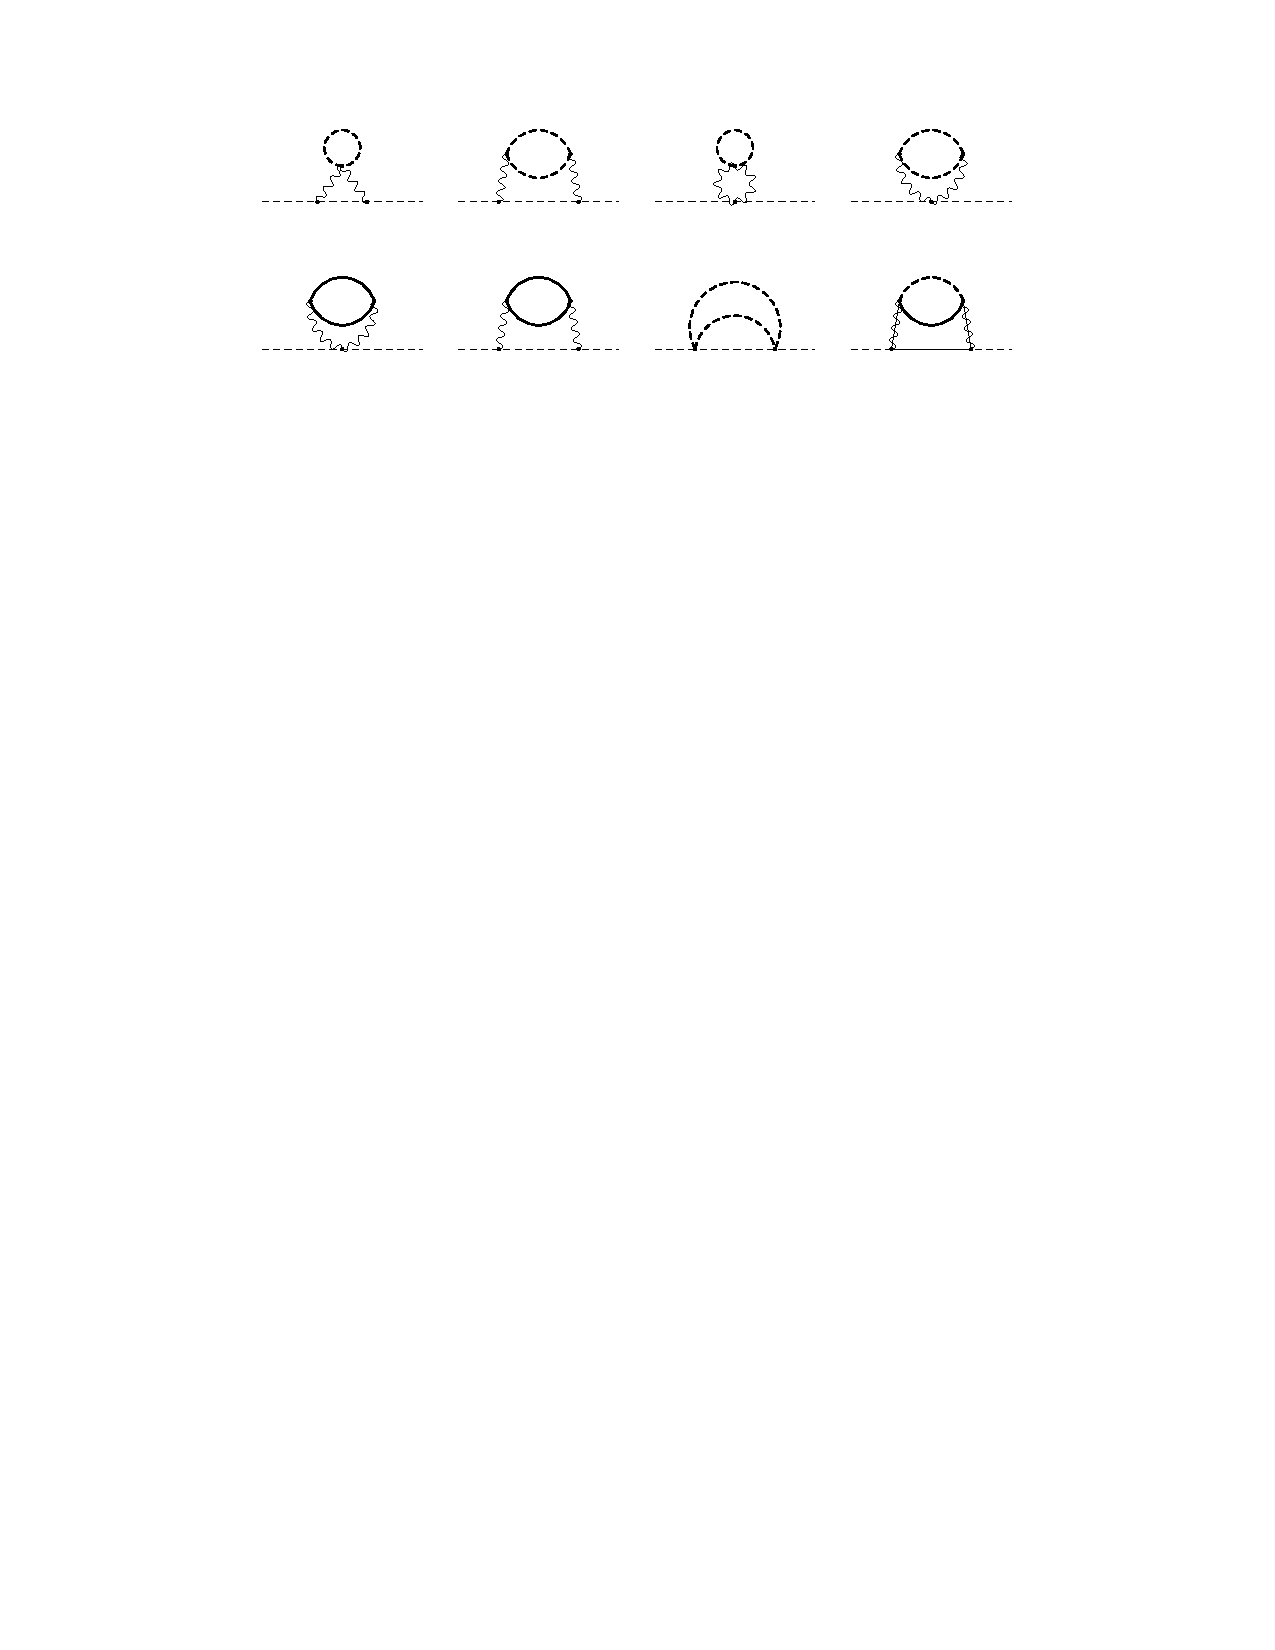
\includegraphics[scale=0.9]{sfermion_GMSB_mass_terms}}
	\\
	\subfloat[Gaugino mass term.  The $\langle S\rangle$ part of the loop is a messenger fermion contribution; the $\langle F_{S}\rangle$ part is a messenger sfermion contribution.  Reprinted from Fig. 6.3 of ref. \cite{SUSY_primer}.]{\label{fig:gaugino_GMSB_mass_term}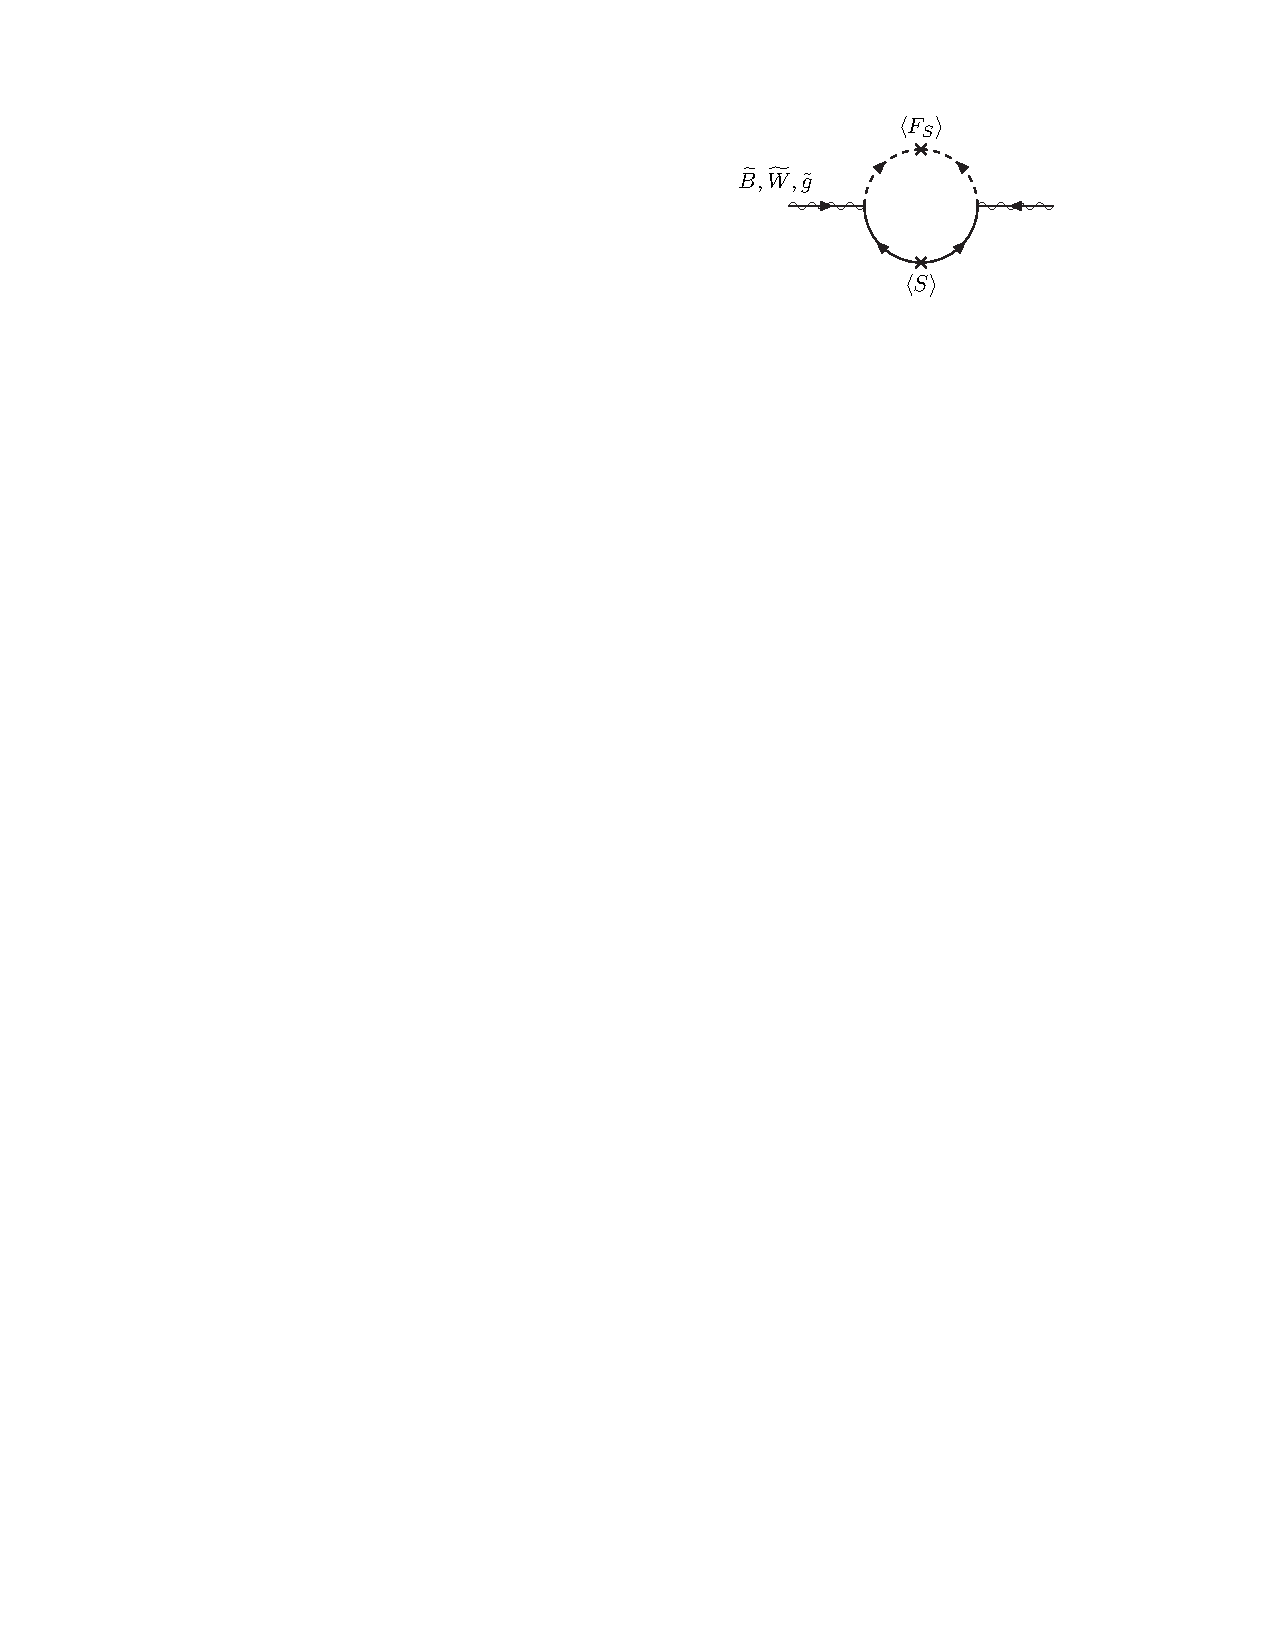
\includegraphics[scale=0.9]{gaugino_GMSB_mass_term}}
	\caption{Contributions to sfermion and gaugino masses from loop interactions with messenger particles in the GMSB framework.}
	\label{fig:gaugino_sfermion_GMSB_mass_terms}
\end{figure}

Historically, GMSB and gravity-mediated SUSY breaking, or mSUGRA \cite{mSUGRA}, have been the two most thoroughly experimentally studied scenarios of SUSY breaking.  One advantage of GMSB over mSUGRA is that it naturally suppresses flavor violation, a generic prediction of supersymmetry.  Flavor violation is introduced in the $\mbox{scalar}^{3}$ couplings and sfermion mass terms of $\mathcal{L}_{\mathrm{soft}}$ (second, third, and fourth lines of Eq.~\ref{eq:L_soft}).  Since $a_{u}^{ij}$, $a_{d}^{ij}$, $a_{e}^{ij}$, $m_{\widetilde{Q}ij}$, $m_{\widetilde{L}ij}$, $m_{\widetilde{\overline{u}}ij}$, $m_{\widetilde{\overline{d}}ij}$, and $m_{\widetilde{\overline{e}}ij}$ are matrices in family space, any nonzero off-diagonal elements will lead to mixing between sfermions of different families.  This can lead, for example, to contributions to the diagram $\mu\rightarrow e\gamma$ (Figure~\ref{fig:muegamma}) exceeding the experimental bounds.  To avoid this disaster, \textit{universality} conditions are assumed:

%should I explain how the sfermions in different families can have different masses anyway?
\begin{eqnarray}
\label{eq:universailty_conditions}
\mathbf{m_{\widetilde{Q}}^{2}} = m_{\widetilde{Q}}^{2}\mathbf{1}\mbox{, }\mathbf{m_{\widetilde{L}}^{2}} = m_{\widetilde{L}}^{2}\mathbf{1}\mbox{, }\mathbf{m_{\widetilde{\overline{u}}}^{2}} = m_{\widetilde{\overline{u}}}^{2}\mathbf{1}\mbox{, }\mathbf{m_{\widetilde{\overline{d}}}^{2}} = m_{\widetilde{\overline{d}}}^{2}\mathbf{1}\mbox{, }\mathbf{m_{\widetilde{\overline{e}}}^{2}} = m_{\widetilde{\overline{e}}}^{2}\mathbf{1}
\end{eqnarray}
%
i.e. all sfermion mass matrices arising from the soft terms are assumed to be proportional to the unit matrix $\mathbf{1}$, such that there can be no flavor mixing from these terms and contributions to flavor-changing processes are drastically reduced.\footnote{Universality also includes some assumptions about the form of $a_{uij}$, $a_{dij}$, and $a_{eij}$ and the stipulation that the soft terms not introduce any CP-violating phases.}  In mSUGRA models, universality is assumed from the beginning, while in GMSB it is a natural consequence of the fact that the sparticle-messenger vertices are flavor-blind.

\begin{figure}
	\centering
	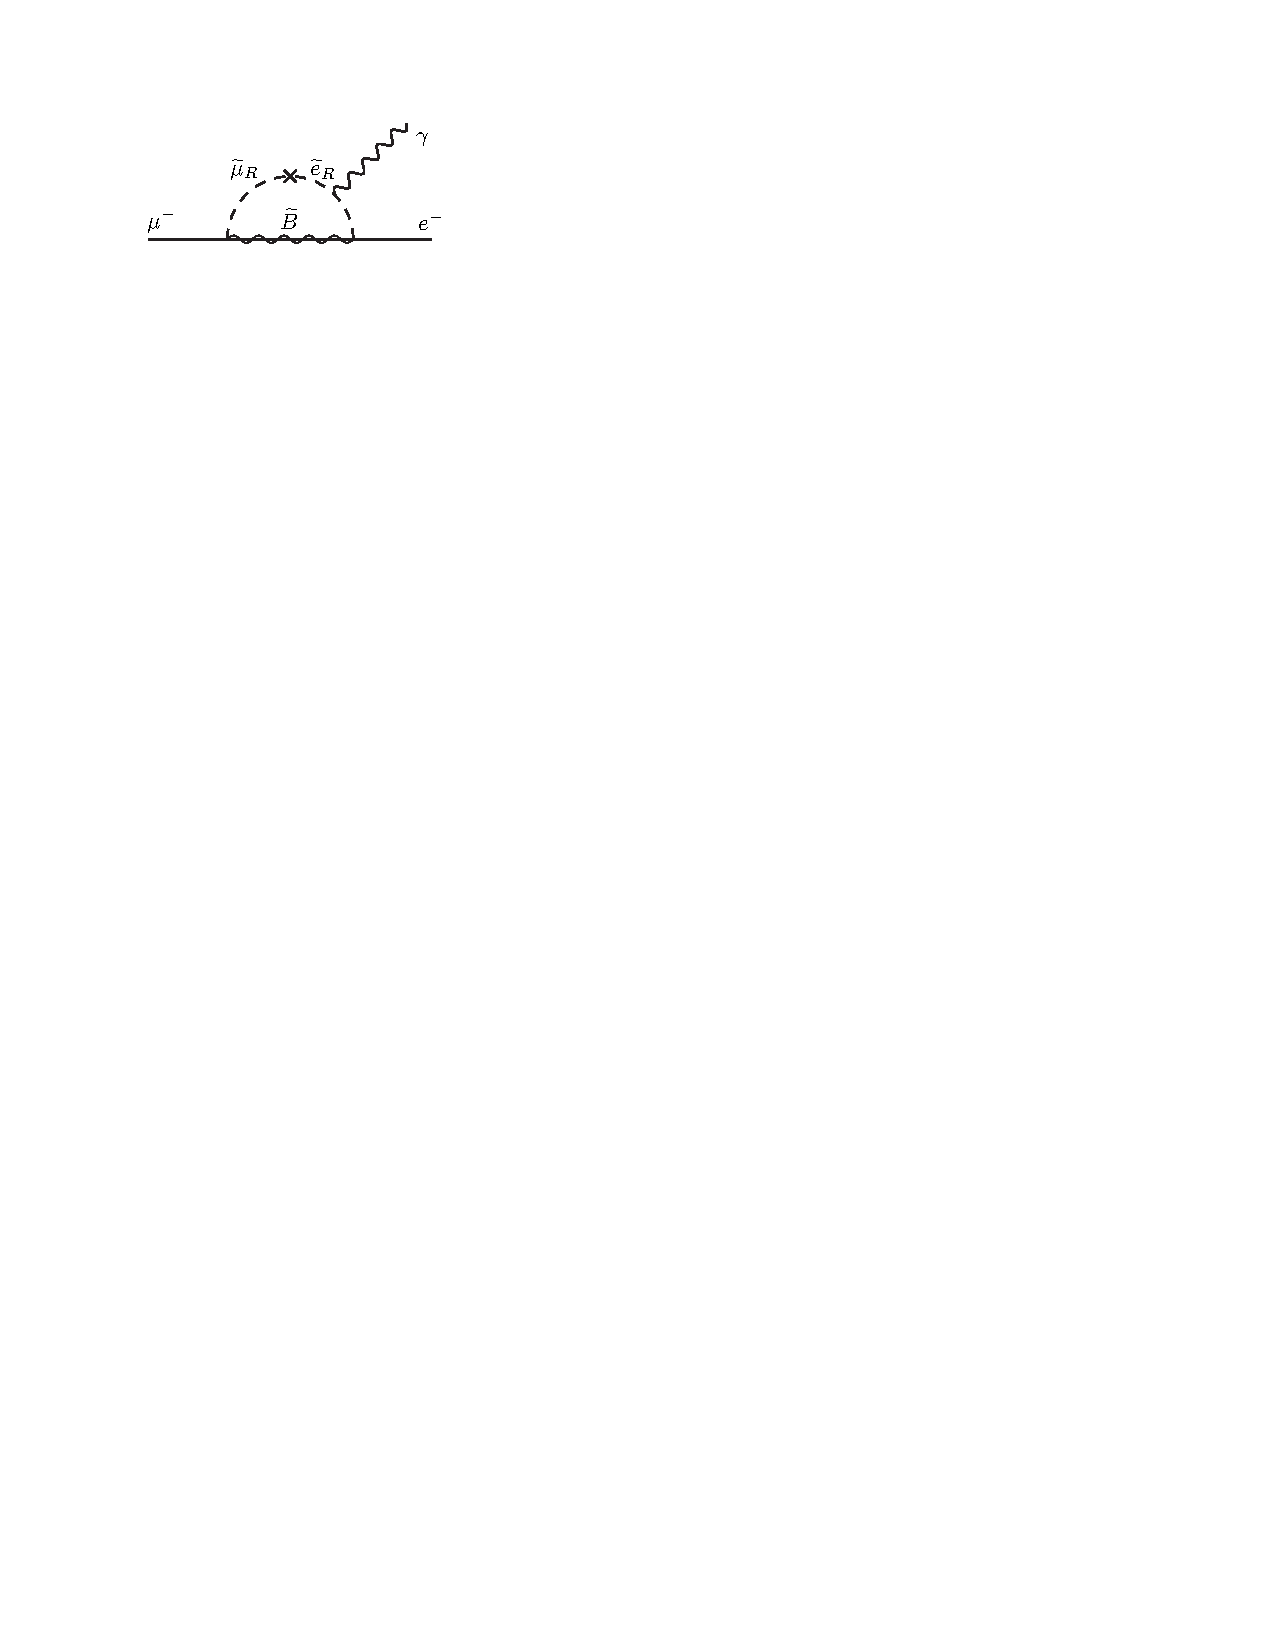
\includegraphics[scale=1.0]{muegamma}
	\caption{Possible contribution to $\mu\rightarrow e\gamma$ from $m_{\widetilde{\overline{e}}ij}$ soft term.  Reprinted from Fig. 5.6(a) of ref. \cite{SUSY_primer}.}
	\label{fig:muegamma}
\end{figure}

In minimal GMSB (mGMSB), there are four messenger supermultiplets $q$, $\overline{q}$, $l$, $\overline{l}$ providing the messenger (s)quarks and (s)leptons.  There is one breaking scale $\Lambda$.  The gaugino masses computed from diagrams like Fig.~\subref*{fig:gaugino_GMSB_mass_term} are given by

\begin{eqnarray}
\label{eq:m_gaugino}
M_{a} &=& \frac{\alpha_{a}}{4\pi}\Lambda
\end{eqnarray}
%
where $a$ runs from 1-3 and the $\alpha_{a}$ are the SM gauge coupling constants.  The sfermion masses computed from diagrams like Fig.~\subref*{fig:sfermion_GMSB_mass_terms} are given by

\begin{eqnarray}
\label{eq:m_sfermion}
m_{\phi_{i}}^{2} &=& 2\Lambda^{2}\sum_{a=1}^{3}(\frac{\alpha_{a}}{4\pi})^{2}C_{a}(i)
\end{eqnarray}
%
where $C_{a}(i)$ are group theory factors that are identical for all particles residing in the same type of supermultiplet (e.g. for all left-handed (s)quarks or left-handed (s)leptons).  As explained in the previous paragraph, the gaugino and sfermion masses do not depend on fermion family.

%cite other GGM papers?
In recent years, much theoretical progress has been made in unifying models of gauge mediation and developing less restrictive models than mGMSB.  \textit{General gauge mediation} (GGM) \cite{Meade_Seiberg_and_Shih} retains the essential features of mGMSB, such as flavor degeneracy and communication of SUSY breaking via messengers, but does not make assumptions about the specific messenger sector or SUSY breaking scale.  Many different collider final states can be interpreted in terms of GGM, and conversely, GGM implies a wealth of signatures, only a small fraction of which have been searched for at colliders \cite{ATLAS_GMSB_1fb-1, CDF_2010_GMSB_paper, CMS_GMSB_1fb-1}.  The following section discusses the aspects of GGM collider phenomenology relevant to this thesis.

\section{Phenomenology of General Gauge Mediation}
\label{sec:Phenomenology of General Gauge Mediation}

The main distinguishing feature of all GMSB phenomenology is that the gravitino $\widetilde{G}$ is very light (eV-keV).  In general, the gravitino mass is proportional to $\langle F\rangle/M_{P}$, where $\langle F\rangle$ is the vacuum expectation value (VEV) of a field $F$ that spontaneously breaks SUSY in the vacuum state and $M_{P}$ is the Planck mass.  In GGM models, $\langle F\rangle \sim 10^{8}$ GeV, leading to a very light gravitino.  In contrast, mSUGRA predicts $\langle F\rangle \sim 10^{20}$ GeV.  The fact that the gravitino is so much lighter than any other particles in the supersymmetric Standard Model, and that it interacts only gravitationally (and thus extremely feebly), leads to two important phenomenological consequences:

\begin{enumerate}
  \item All sparticle decay chains end with the production of a gravitino.
  \item The gravitino escapes 4$\pi$, hermetic collider detectors without interacting, leaving a signature of ``missing" momentum transverse to the beam direction.
\end{enumerate}

Even if the gravitino were lighter than any other sparticle, but heavier than an ordinary SM particle, it still could not decay to the SM particle due to \textit{R-parity}.  R-parity is a conserved quantity of the supersymmetric Standard Model that enforces baryon and lepton number conservation, which would otherwise be generically allowed at levels in conflict with experiment (e.g. the non-observation of baryon- and lepton-number-violating proton decay).  All sparticles have R-parity -1, while all ordinary SM particles have R-parity +1, and R-parity conservation dictates that at any vertex, the product of the R-parities of each leg must be +1.  This leads to two more important consequences:

\begin{enumerate}
  \item Since conservation of energy only allows it to decay to ordinary SM particles, but R-parity prevents a sparticle-particle-particle vertex, the \textit{lightest supersymmetric particle} (LSP) must be absolutely stable.  All sparticle decays proceed through the \textit{next-to-lightest supersymmetric particle} (NLSP), which in turn decays to the LSP.  The fact that it is stable and only gravitationally interacting makes the gravitino a candidate dark matter particle (see Sec.~\ref{sec:Experimental Status of SUSY}).
  \item In colliders, sparticles are produced in pairs (particle + particle $\rightarrow$ sparticle + sparticle).
\end{enumerate}

In GMSB, then, the gravitino is the LSP.  If the NLSP is a gaugino,\footnote{In principle, the NLSP could be anything, but in most popular GGM models, it is either a gaugino or a stau.  The stau NLSP search is not the subject of this thesis, so it will not be considered in this section.} then the possible decays depend on mixing among the gauginos.  Due to the effects of EWSB, the four neutral gauginos $\widetilde{H}_{u}^{0}$, $\widetilde{H}_{d}^{0}$, $\widetilde{B}$, $\widetilde{W}^{0}$ mix into four \textit{neutralino} mass eigenstates $\NLSP, \widetilde{\chi}_{2}^{0}, \widetilde{\chi}_{3}^{0}, \widetilde{\chi}_{4}^{0}$, and the four charged gauginos $\widetilde{H}_{u}^{+}$, $\widetilde{H}_{d}^{-}$, $\widetilde{W}^{+}$, $\widetilde{W}^{-}$ mix into two \textit{chargino} mass eigenstates $\widetilde{\chi}_{1}^{\pm}, \widetilde{\chi}_{2}^{\pm}$ (two mass eigenstates each with two possible charges = four particles).  In the limit that EWSB effects are small, the neutralino and chargino masses can be written as the gauge eigenstate masses plus a small perturbation:

\begin{eqnarray}
\label{eq:neutralino_chargino_masses}
m_{\NLSP} &=& M_{1}\mbox{ }-\mbox{ }\frac{m_{Z}^{2}\sin^{2}\theta_{W}(M_{1} + \mu\sin 2\beta)}{\mu^{2} - M_{1}^{2}}\mbox{ + }...\\
m_{\widetilde{\chi}_{2}^{0}} &=& M_{2}\mbox{ }-\mbox{ }\frac{m_{W}^{2}(M_{2} + \mu\sin 2\beta)}{\mu^{2} - M_{2}^{2}}\mbox{ + }...\\
m_{\widetilde{\chi}_{3}^{0}} &=& |\mu|\mbox{ + }\frac{m_{Z}^{2}(\sgn(\mu) - \sin 2\beta)(\mu + M_{1}\cos^{2}\theta_{W} + M_{2}\sin^{2}\theta_{W})}{2(\mu + M_{1})(\mu + M_{2})}\mbox{ + }...\\
m_{\widetilde{\chi}_{4}^{0}} &=& |\mu|\mbox{ + }\frac{m_{Z}^{2}(\sgn(\mu) + \sin 2\beta)(\mu - M_{1}\cos^{2}\theta_{W} - M_{2}\sin^{2}\theta_{W})}{2(\mu - M_{1})(\mu - M_{2})}\mbox{ + }...\\
m_{\widetilde{\chi}_{1}^{\pm}} &=& M_{2}\mbox{ }-\mbox{ }\frac{m_{W}^{2}(M_{2} + \mu\sin 2\beta)}{\mu^{2} - M_{2}^{2}}\mbox{ + }...\\
m_{\widetilde{\chi}_{2}^{\pm}} &=& |\mu|\mbox{ + }\frac{m_{W}^{2}\sgn(\mu)(\mu + M_{2}\sin 2\beta)}{\mu^{2} - M_{2}^{2}}\mbox{ + }...
\end{eqnarray}
%
where $\tan\beta = \langle H_{u}^{0}\rangle/\langle H_{d}^{0}\rangle$.

The two scenarios studied in ref. \cite{CMS_GMSB_1fb-1} are the following:

\begin{itemize}
  \item \textbf{Bino NLSP}: $M_{1} \sim$ few hundred GeV, $M_{2}, |\mu| \gg M_{1}$.  All but the lightest neutralino are effectively inaccessible at the LHC due to their large masses.  The NLSP can always decay to $\gamma + \widetilde{G}$, and if it is heavy enough, to $Z + \widetilde{G}$ or $H + \widetilde{G}$.
  \item \textbf{Wino NLSP}: $M_{2} \sim$ few hundred GeV, $M_{1}, |\mu| \gg M_{2}$.  The lightest neutralino and the lightest chargino are nearly degenerate in mass, and are the only two particles to play a role at the LHC.  The decays described in the previous bullet point can happen, as well as chargino decays to $W + \widetilde{G}$.
\end{itemize}
%
The subject of this thesis is the classic bino NLSP decay $\gamma + \widetilde{G}$.

Since strong production of SUSY particles dominates over electroweak production at the LHC due to the enhanced $gg$ parton luminosity over the $q\overline{q}$ parton luminosity, early LHC searches are particularly sensitive to light squarks and gluinos.  General gauge mediation makes no a priori restrictions on the mass splitting between the strongly interacting sparticles and the weakly interacting sparticles, so models with light squarks and gluinos are viable.  In fact, such models could not be probed as well at the Tevatron\footnote{Located on the Fermilab site in Batavia, Illinois, the Tevatron was a proton-antiproton collider operating at 1.96 TeV center-of-mass energy.  The Tevatron ran from 1987 to 2011 \cite{Tevatron_lifetime}.} as they are at the LHC due to the aforementioned parton luminosities.

Typical LHC signatures of the bino and wino NLSP scenarios are shown in Figure~\ref{fig:bino_wino_NLSP_signatures}.

\begin{figure}
	\centering
	\subfloat[Two gluinos each decay via $\NLSP\rightarrow\gamma\widetilde{G}$.]{\label{fig:2photons_jets_MET}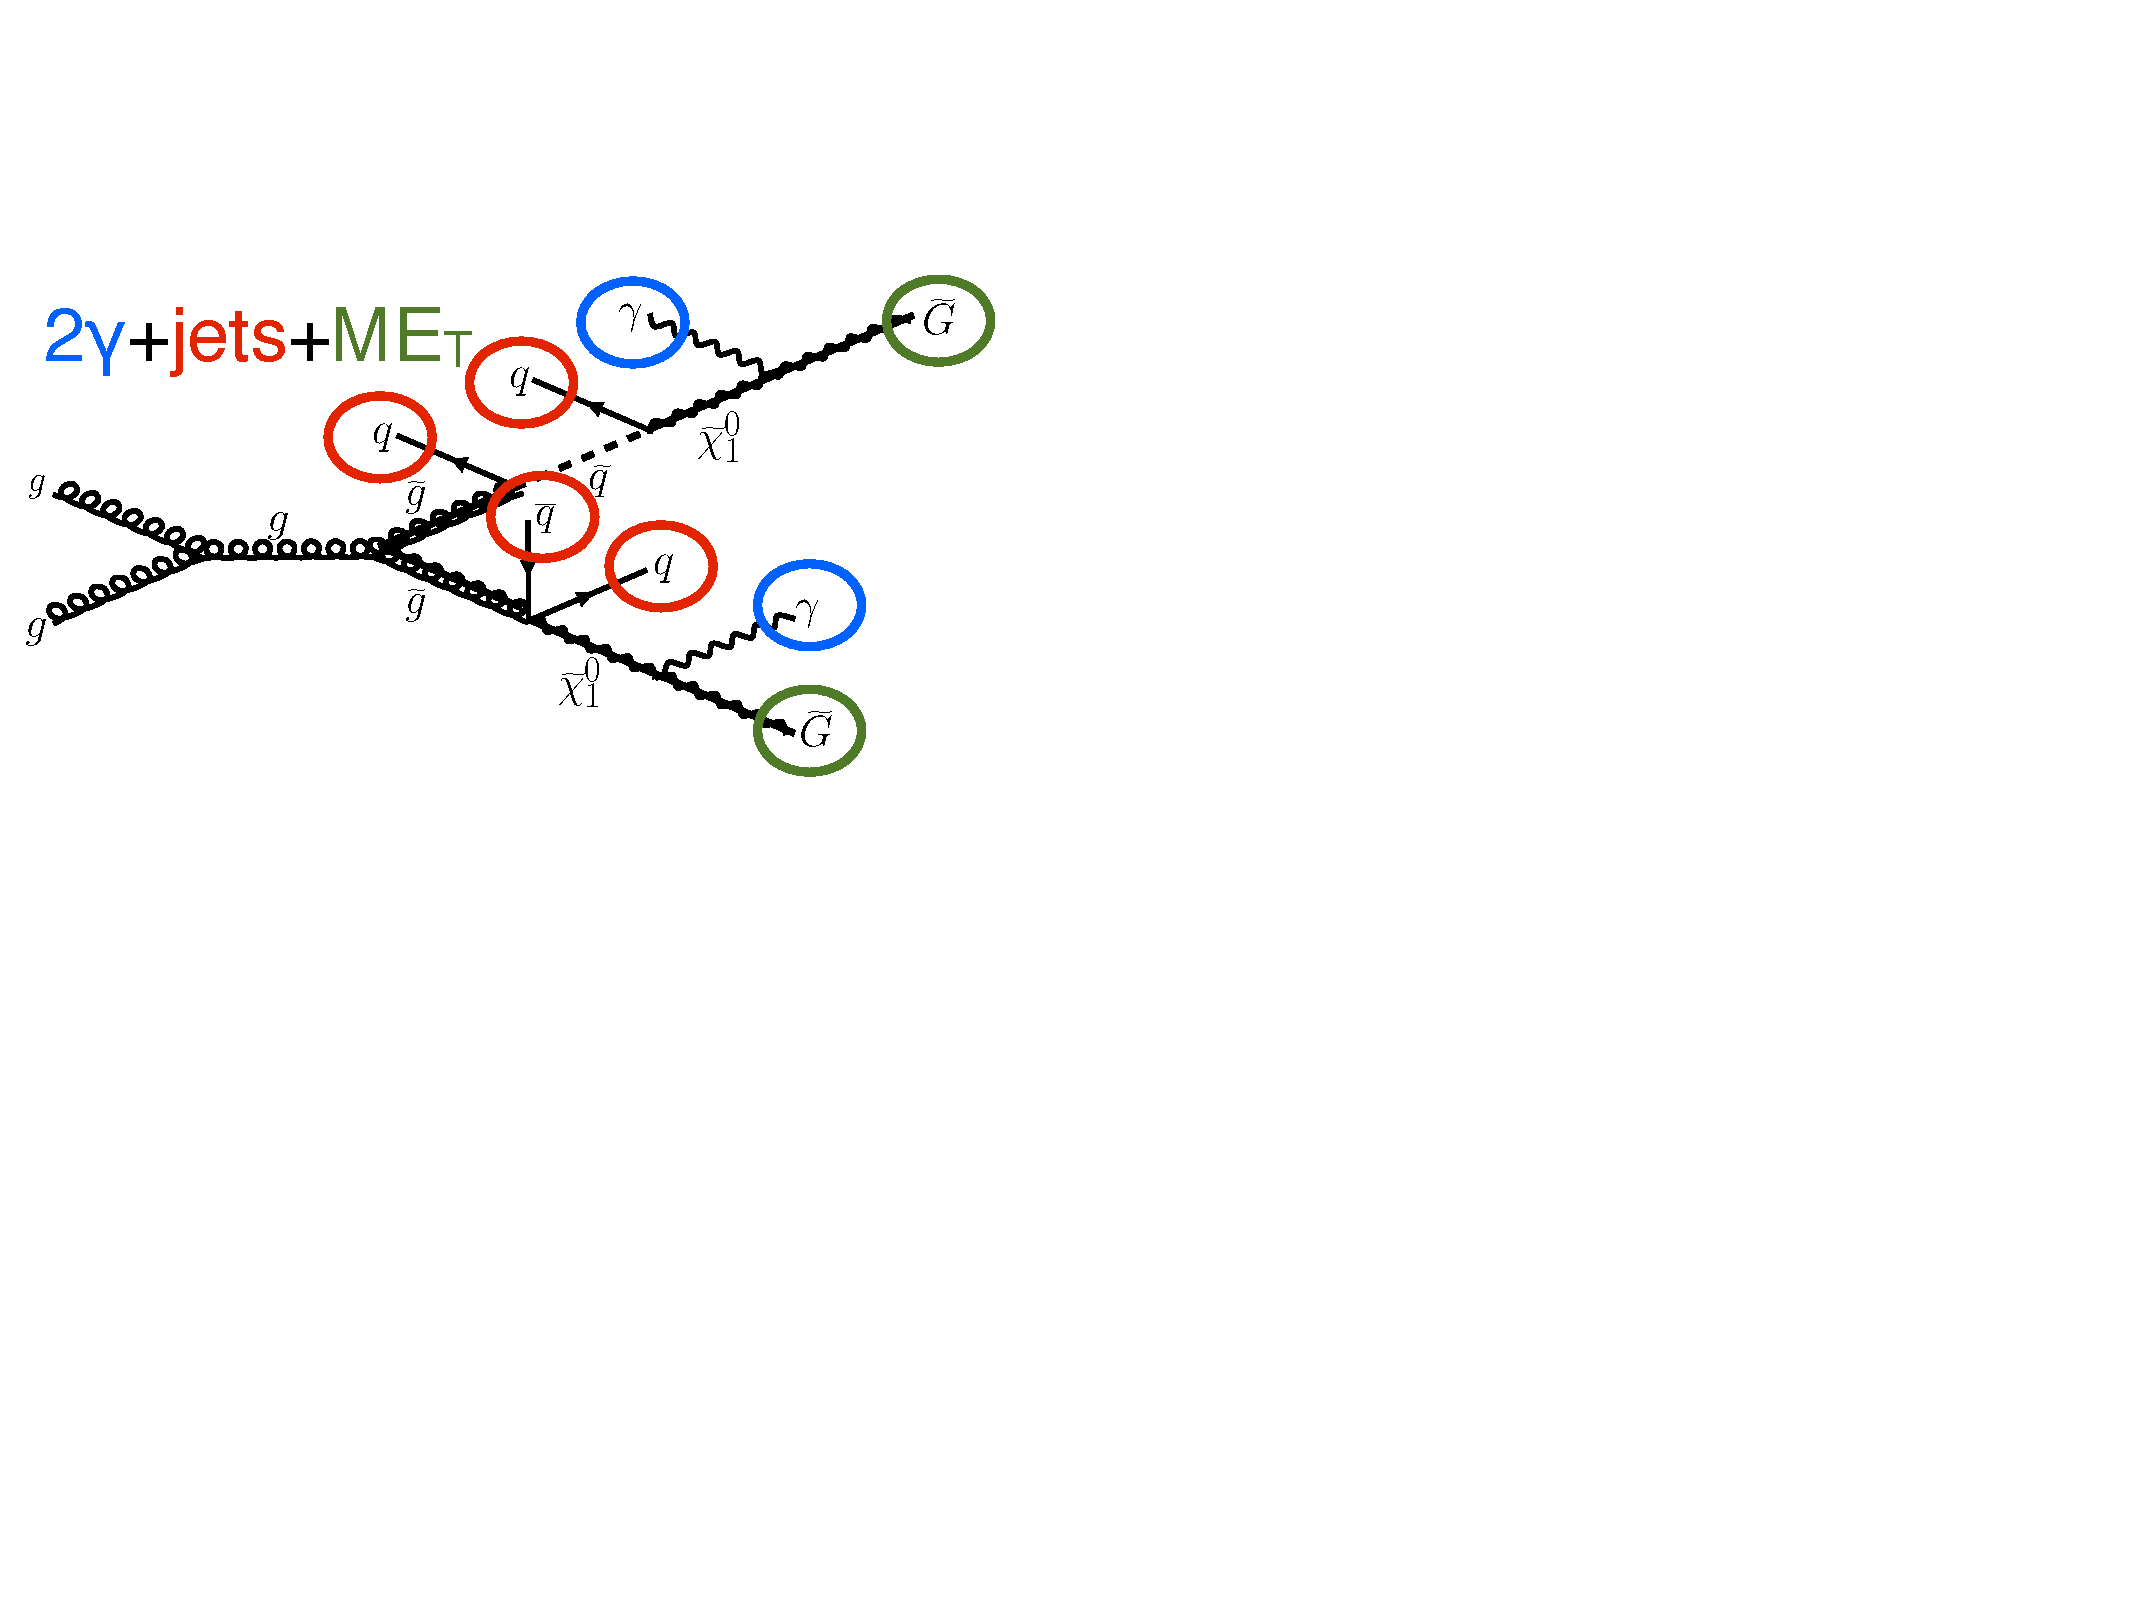
\includegraphics[scale=0.4]{2photons_jets_MET}}
	\hspace{1cm}
	\subfloat[One gluino decays via $\NLSP\rightarrow\gamma\widetilde{G}$, the other via $\NLSP\rightarrow Z(\rightarrow q\overline{q})\widetilde{G}$.]{\label{fig:bino_photon_jets_MET}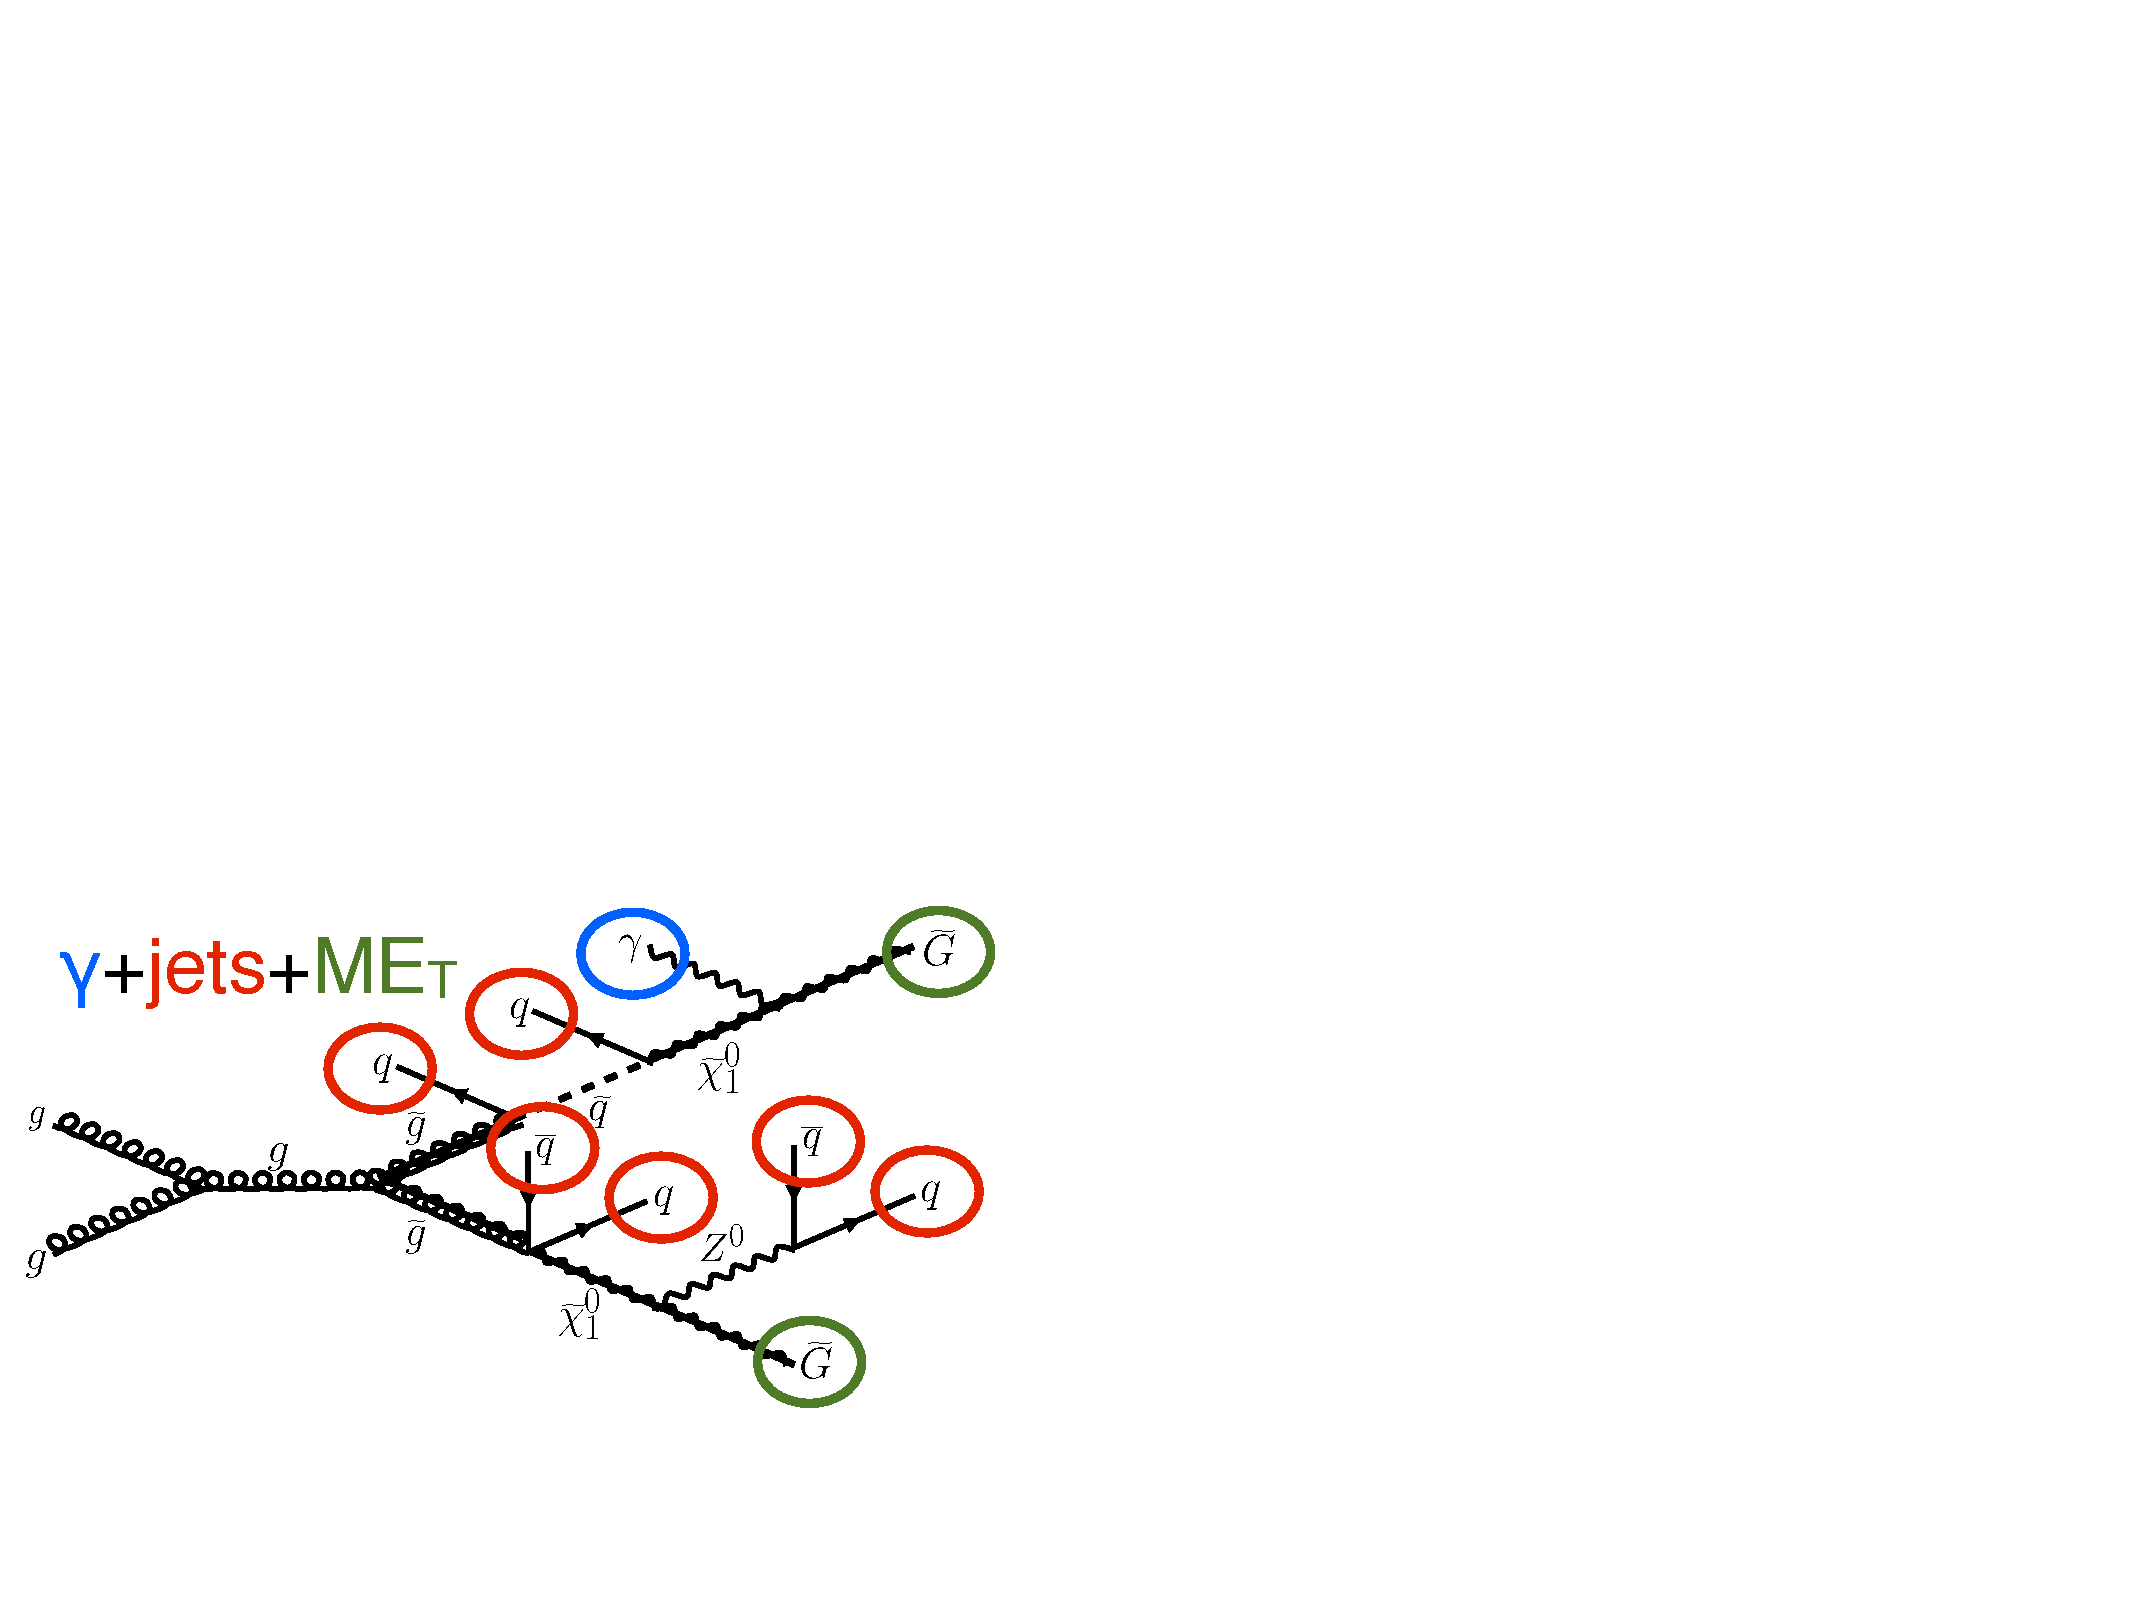
\includegraphics[scale=0.4]{bino_photon_jets_MET}}
	\\
	\subfloat[One gluino decays via $\NLSP\rightarrow\gamma\widetilde{G}$, the other via $\chi_{1}^{\pm}\rightarrow W^{\pm}(\rightarrow l^{\pm}\nu_{l})\widetilde{G}$.]{\label{fig:lepton_photon_jets_MET}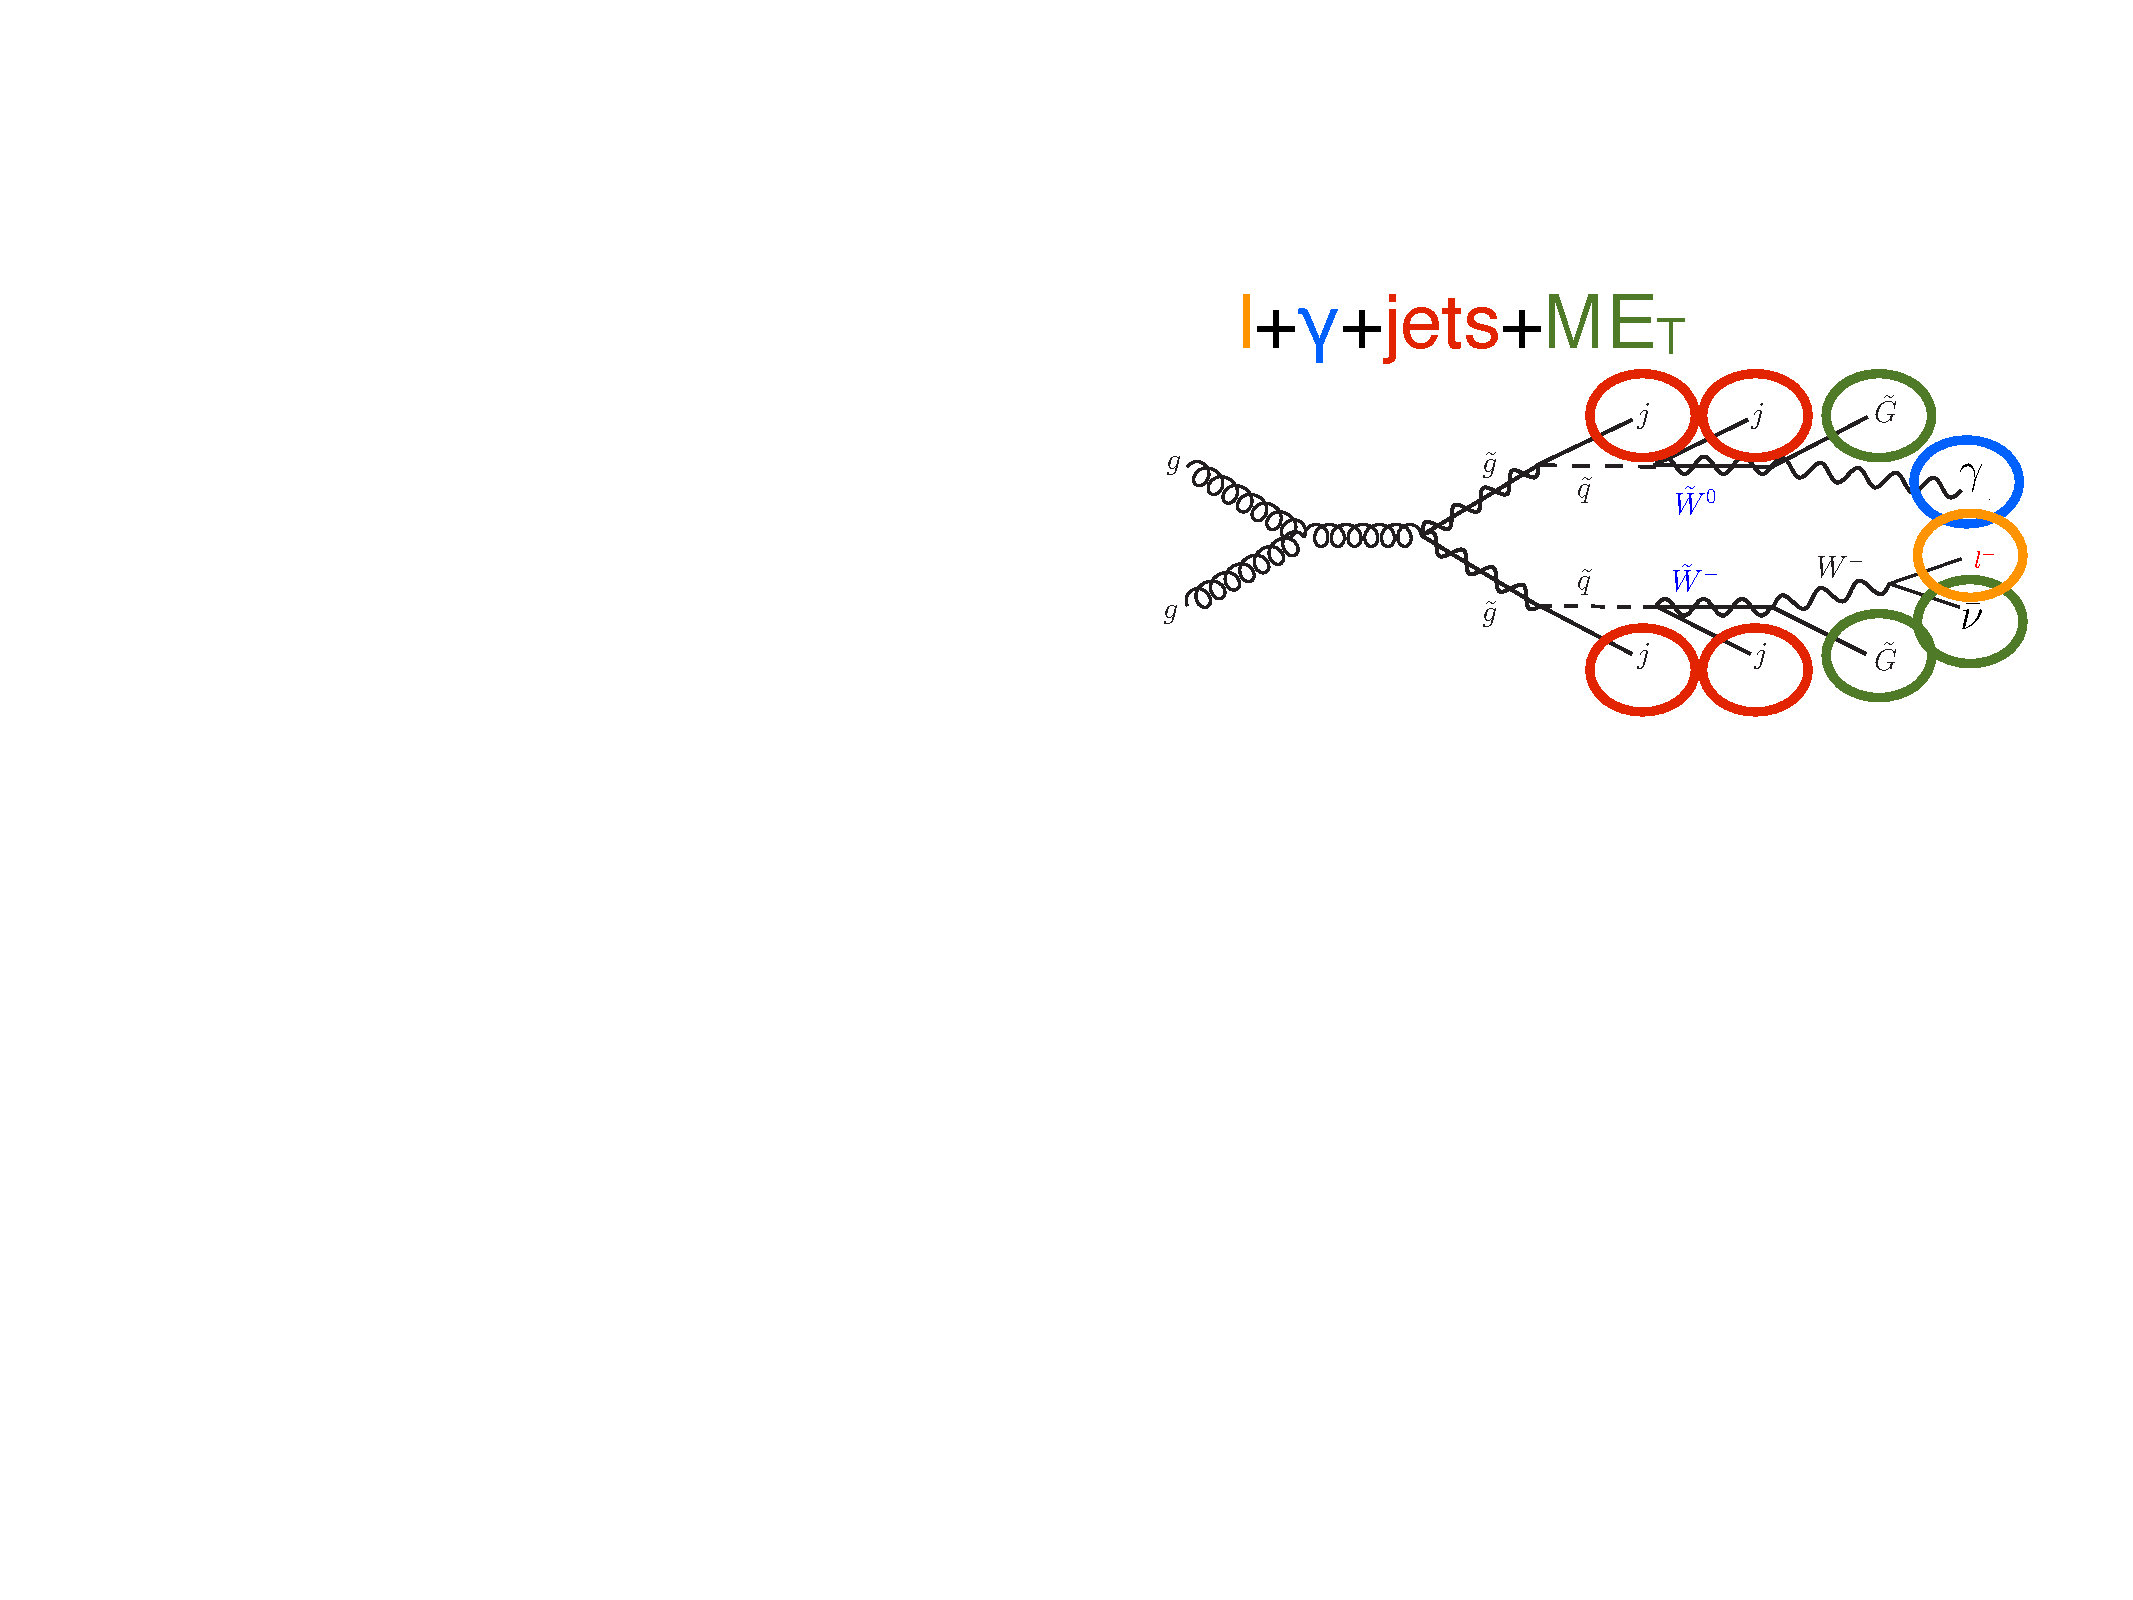
\includegraphics[scale=0.4]{lepton_photon_jets_MET}}
	\hspace{1cm}
	\subfloat[One gluino decays via $\NLSP\rightarrow\gamma\widetilde{G}$, the other via $\chi_{1}^{\pm}\rightarrow W^{\pm}(\rightarrow q\overline{q}^{'})\widetilde{G}$.]{\label{fig:wino_photon_jets_MET}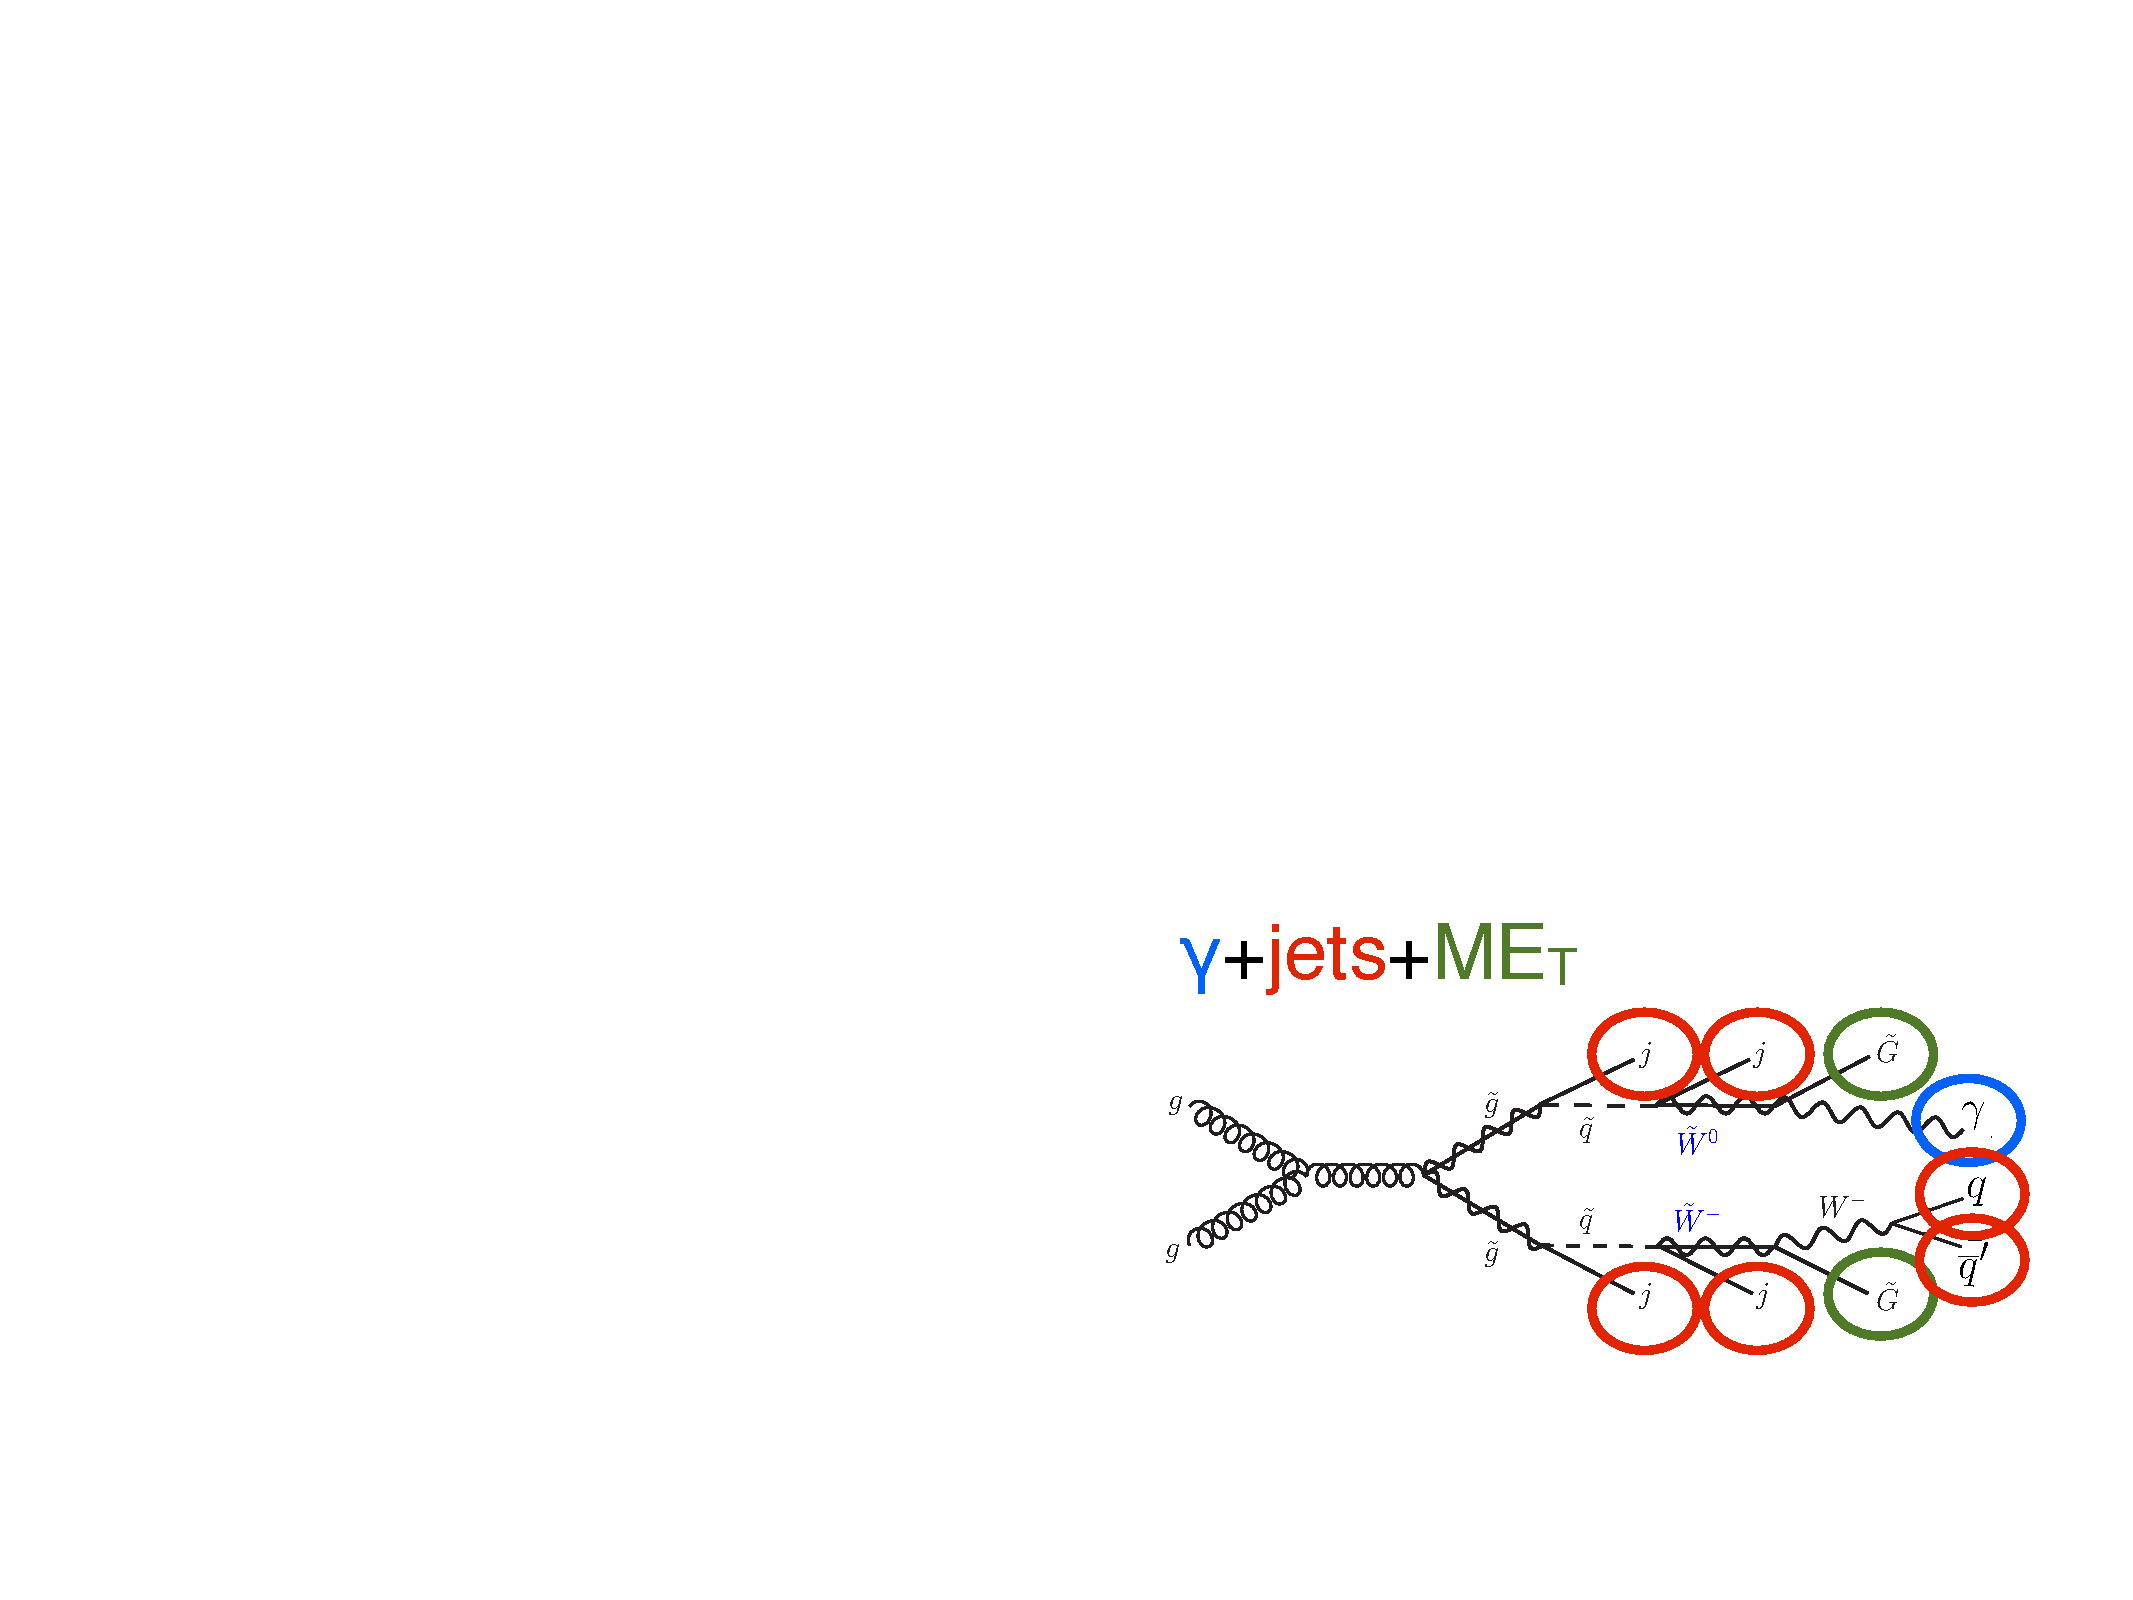
\includegraphics[scale=0.4]{wino_photon_jets_MET}}
	\caption{Typical LHC signatures of the bino and wino NLSP scenarios.}
	\label{fig:bino_wino_NLSP_signatures}
\end{figure}

\section{Experimental Status of SUSY}
\label{sec:Experimental Status of SUSY}

Collider searches for evidence of supersymmetry began in earnest in the 1980s \cite{SUSY_history} and continue to this day.  Most recently, the LHC and Tevatron experiments have set the strictest limits on a variety of SUSY breaking scenarios, including GMSB and mSUGRA.

Figure~\ref{fig:CMS_SUSY_2011Limits_tanb10} shows the current limits set by the CMS experiment on the mSUGRA model (with tan $\beta$ = 10) in the $m_{0}$-$m_{1/2}$ plane.  (Note that although the plot is truncated at $m_{0}$ = 1000 GeV/$\mbox{c}^{2}$, some searches are sensitive out to $m_{0} \sim$ 2000 GeV/$\mbox{c}^{2}$.)  Although the LHC has pushed $m_{0}$ above $\sim$1 TeV/$\mbox{c}^{2}$ for $m_{1/2}$ up to $\sim$400 GeV/$\mbox{c}^{2}$, casting some doubt onto the theory's prospects for solving the hierarchy problem, there is still a sizable chunk of mSUGRA parameter space that is not ruled out by collider experiments.  Furthermore, parts of the CMS unexplored regions overlap with areas allowed by astrophysics experiments \cite{CMSSM_fits}.

\begin{figure}
	\centering
	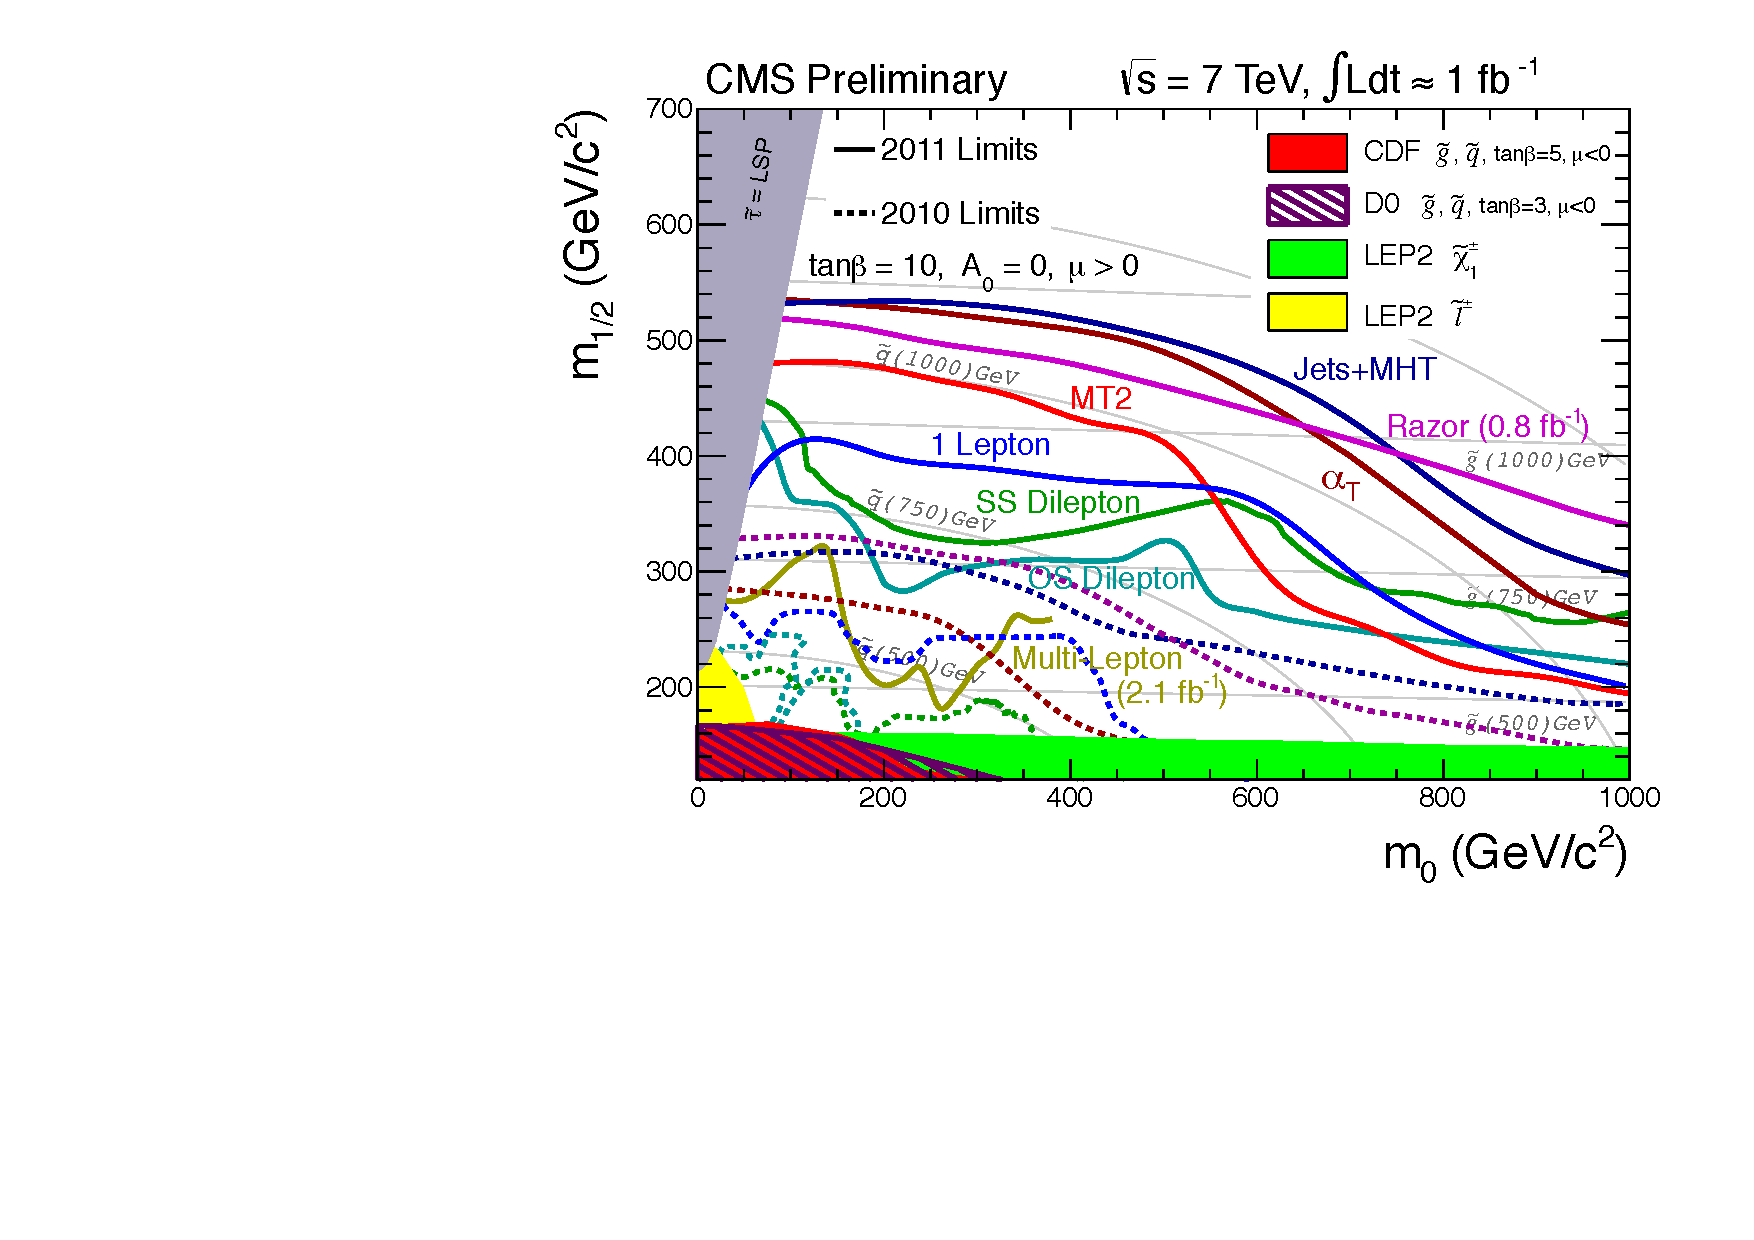
\includegraphics[scale=0.6]{CMS_SUSY_2011Limits_tanb10}
	\caption{CMS limits on mSUGRA with tan $\beta$ = 10.  The limits set by individual searches are shown as separate colored lines.  Solid lines refer to 2011 searches (i.e. using an integrated luminosity of $\sim$1 $\mbox{fb}^{-1}$), while dashed lines refer to 2010 searches ($\sim$36 $\mbox{pb}^{-1}$).  Reprinted from ref. \cite{CMS_mSUGRA}.}
	\label{fig:CMS_SUSY_2011Limits_tanb10}
\end{figure}

%check this whole paragraph and figures from ATLAS!
Figure~\ref{fig:ATLAS_SPS8_limit} shows the most up-to-date limit (using 1 $\mbox{fb}^{-1}$ of integrated luminosity collected by the ATLAS experiment \cite{ATLAS} at the LHC) on the Snowmass Points and Slopes (SPS) model of mGMSB, dubbed SPS8 \cite{SPS}.  The best limits on a variety of GGM models, from the same ATLAS study, are shown in Figure~\ref{fig:ATLAS_GGM_limit}.  In these models, no assumptions are made about the specific parameters common to many gauge mediation models (e.g. the number of messengers or the relationship between the messenger mass and the SUSY breaking scale).  Instead, it is only assumed that the lightest neutralino is light enough to be produced on-shell at the LHC (by setting $\mbox{M}_{1}$ and $\mbox{M}_{2}$ appropriately, see Sec.~\ref{sec:Phenomenology of General Gauge Mediation}) and that it decays to a gravitino, that the gravitino is extremely relativistic (mass of order eV-keV), and that the gravitino is stable.  The one-dimensional scan over SUSY breaking scales in the SPS8 model (in which the full sparticle spectrum is specified by the model parameters) is replaced by a two-dimensional scan over gluino and lightest neutralino mass in the GGM models (in which all sparticles except the gluino, first- and second-generation squarks, and neutralinos are forced to be at $\sim$1.5 TeV/$\mbox{c}^{2}$, effectively decoupling them from the dynamics that can be probed with 1 $\mbox{fb}^{-1}$ at a 7 TeV/c pp collider).
%maybe repeat some of this in the earlier section about the advantages of simplified models (can make a more logical, clear mapping between search strategy and model sensitivity, can be less model-dependent)

\begin{figure}
	\centering
	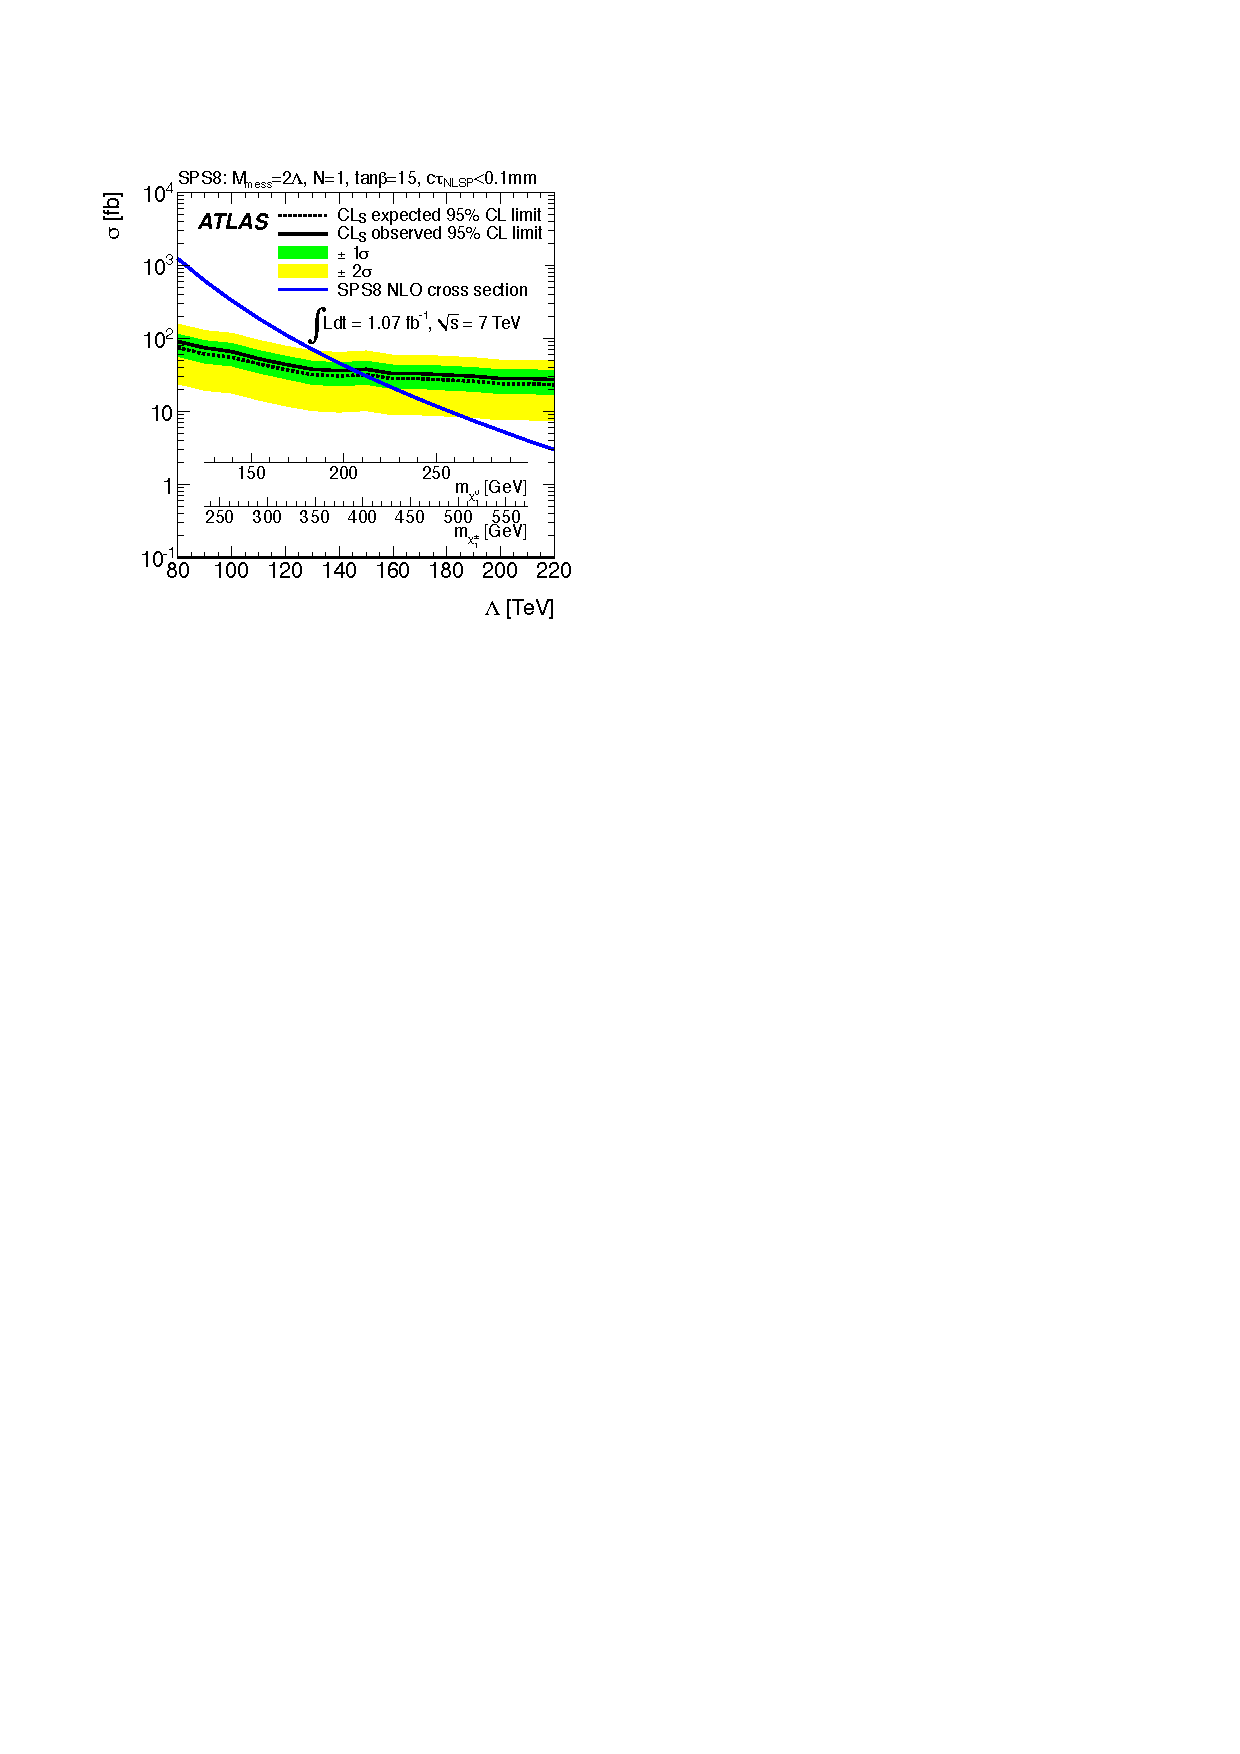
\includegraphics[scale=0.9]{ATLAS_SPS8_limit}
	\caption{ATLAS cross section upper limit on the SPS8 \cite{SPS} model of mGMSB as a function of SUSY breaking scale $\Lambda$, lightest neutralino mass $\mbox{m}_{\NLSP}$, or lightest chargino mass $\mbox{m}_{\widetilde{\chi}_{1}^{\pm}}$.  Values of $\Lambda$, $\mbox{m}_{\NLSP}$, or $\mbox{m}_{\widetilde{\chi}_{1}^{\pm}}$ below the intersection point between the blue (predicted SPS8 cross section) and black (observed cross section upper limit) curves are excluded.  The model parameters listed above the plot are defined in Secs.~\ref{sec:Gauge-Mediated SUSY Breaking} and~\ref{sec:Phenomenology of General Gauge Mediation}, except for $\tau_{\mathrm{NLSP}}$, which is the neutralino lifetime.  Reprinted from ref. \cite{ATLAS_GMSB_1fb-1}.}
	\label{fig:ATLAS_SPS8_limit}
\end{figure}

\begin{figure}
	\centering
	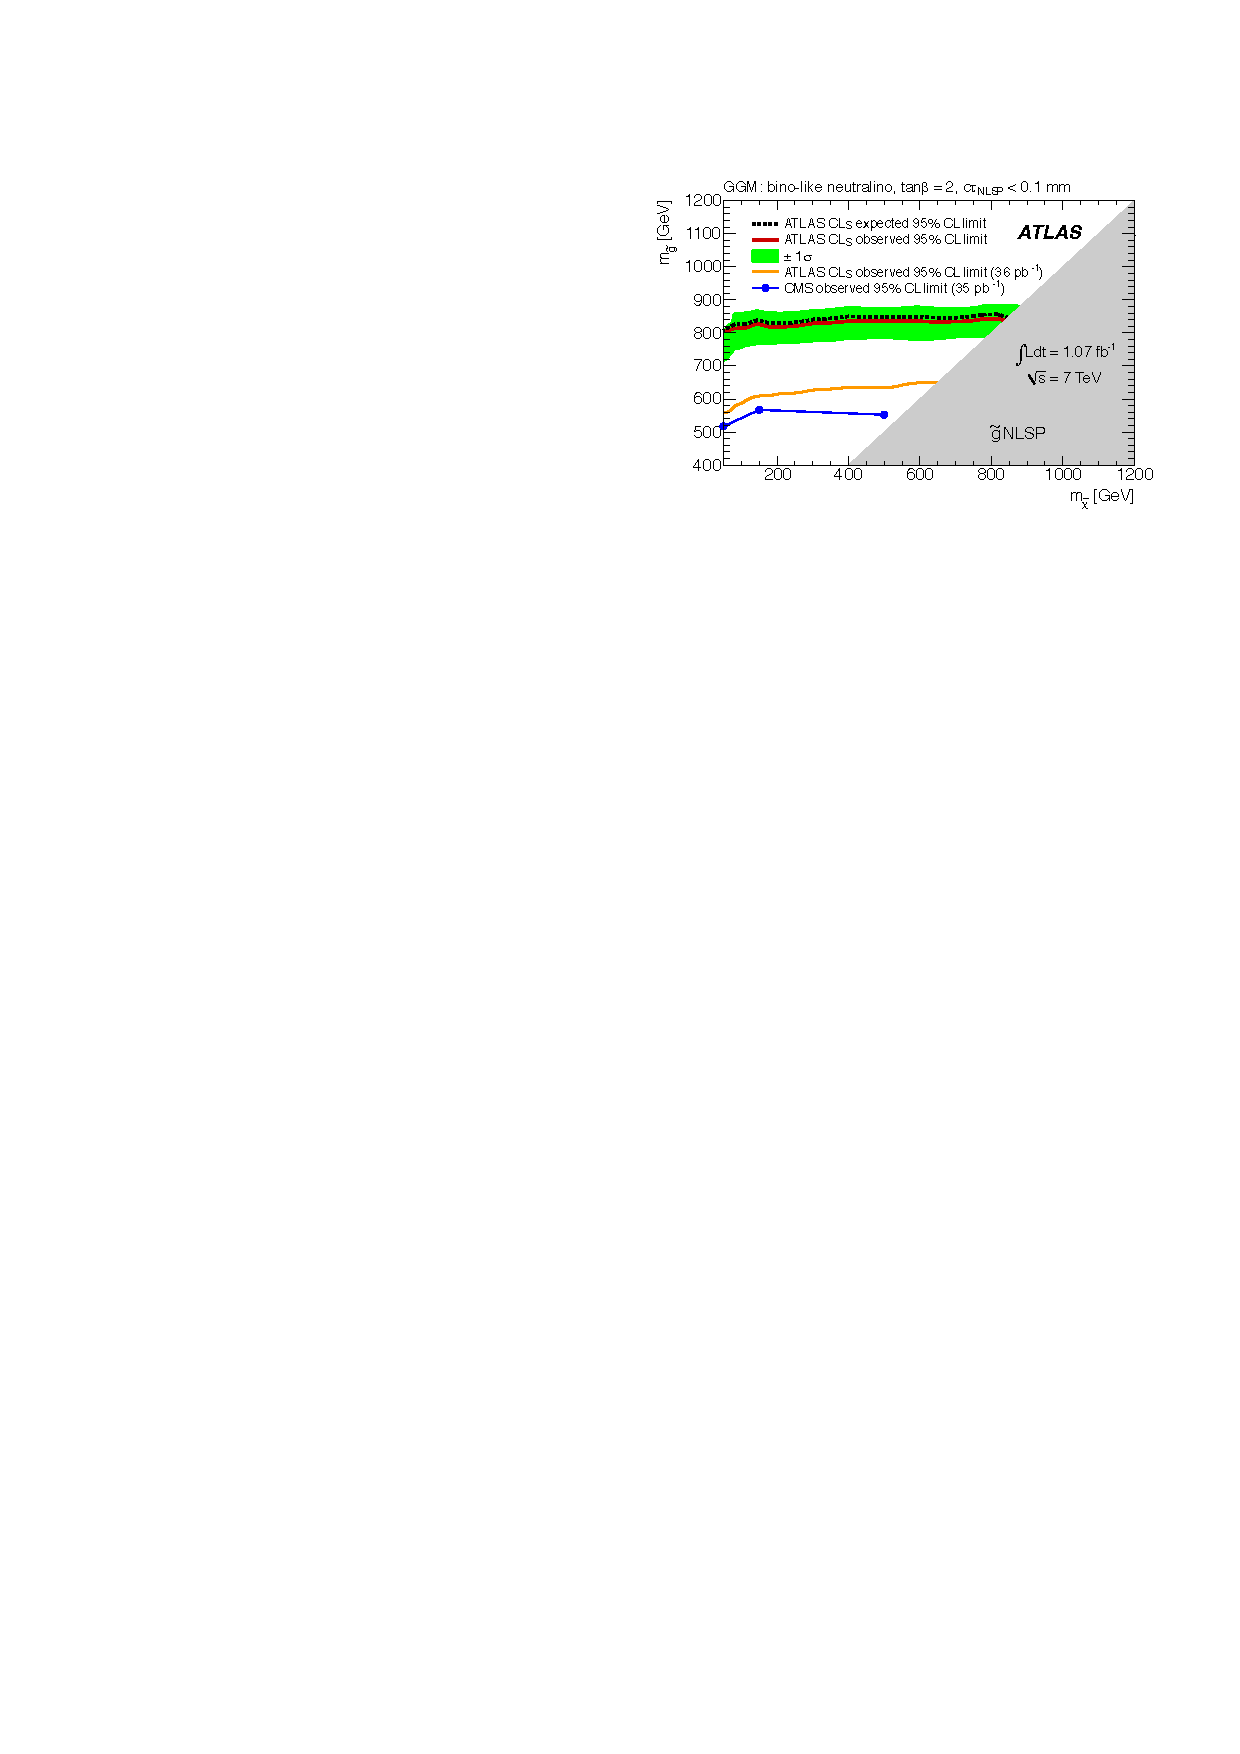
\includegraphics[scale=0.9]{ATLAS_GGM_limit}
	\caption{ATLAS exclusion contour in the $m_{\widetilde{g}}$-$m_{\NLSP}$ plane.  Values of $m_{\widetilde{g}}$-$m_{\NLSP}$ below the red curve are excluded.  The gray region is theoretically excluded in the GGM models considered.  ``Bino-like neutralino" means that $M_{2}$ = 1.5 TeV/$\mbox{c}^{2}$.  Reprinted from ref. \cite{ATLAS_GMSB_1fb-1}.}
	\label{fig:ATLAS_GGM_limit}
\end{figure}

In general, the lifetime of the lightest neutralino in GMSB models can take on any value between hundreds of nanometers to a few kilometers depending on the mass of the lightest neutralino and the SUSY breaking scale \cite{SUSY_primer}.  The search published in ref. \cite{ATLAS_GMSB_1fb-1} (from which Figs.~\ref{fig:ATLAS_SPS8_limit} and~\ref{fig:ATLAS_GGM_limit} are culled) considers only \textit{prompt} neutralino variants, i.e. with neutralino lifetime short enough that the distance traveled by the neutralino before decay cannot be resolved by the detector.  The most recent limits on non-prompt SPS8-style neutralino models were set by the Collider Detector at Fermilab (CDF) collaboration with 570 $\mbox{pb}^{-1}$, and are shown in Figure~\ref{fig:CDF_lifetime_vs_mass} \cite{CDF_2010_GMSB_paper}.

\begin{figure}
	\centering
	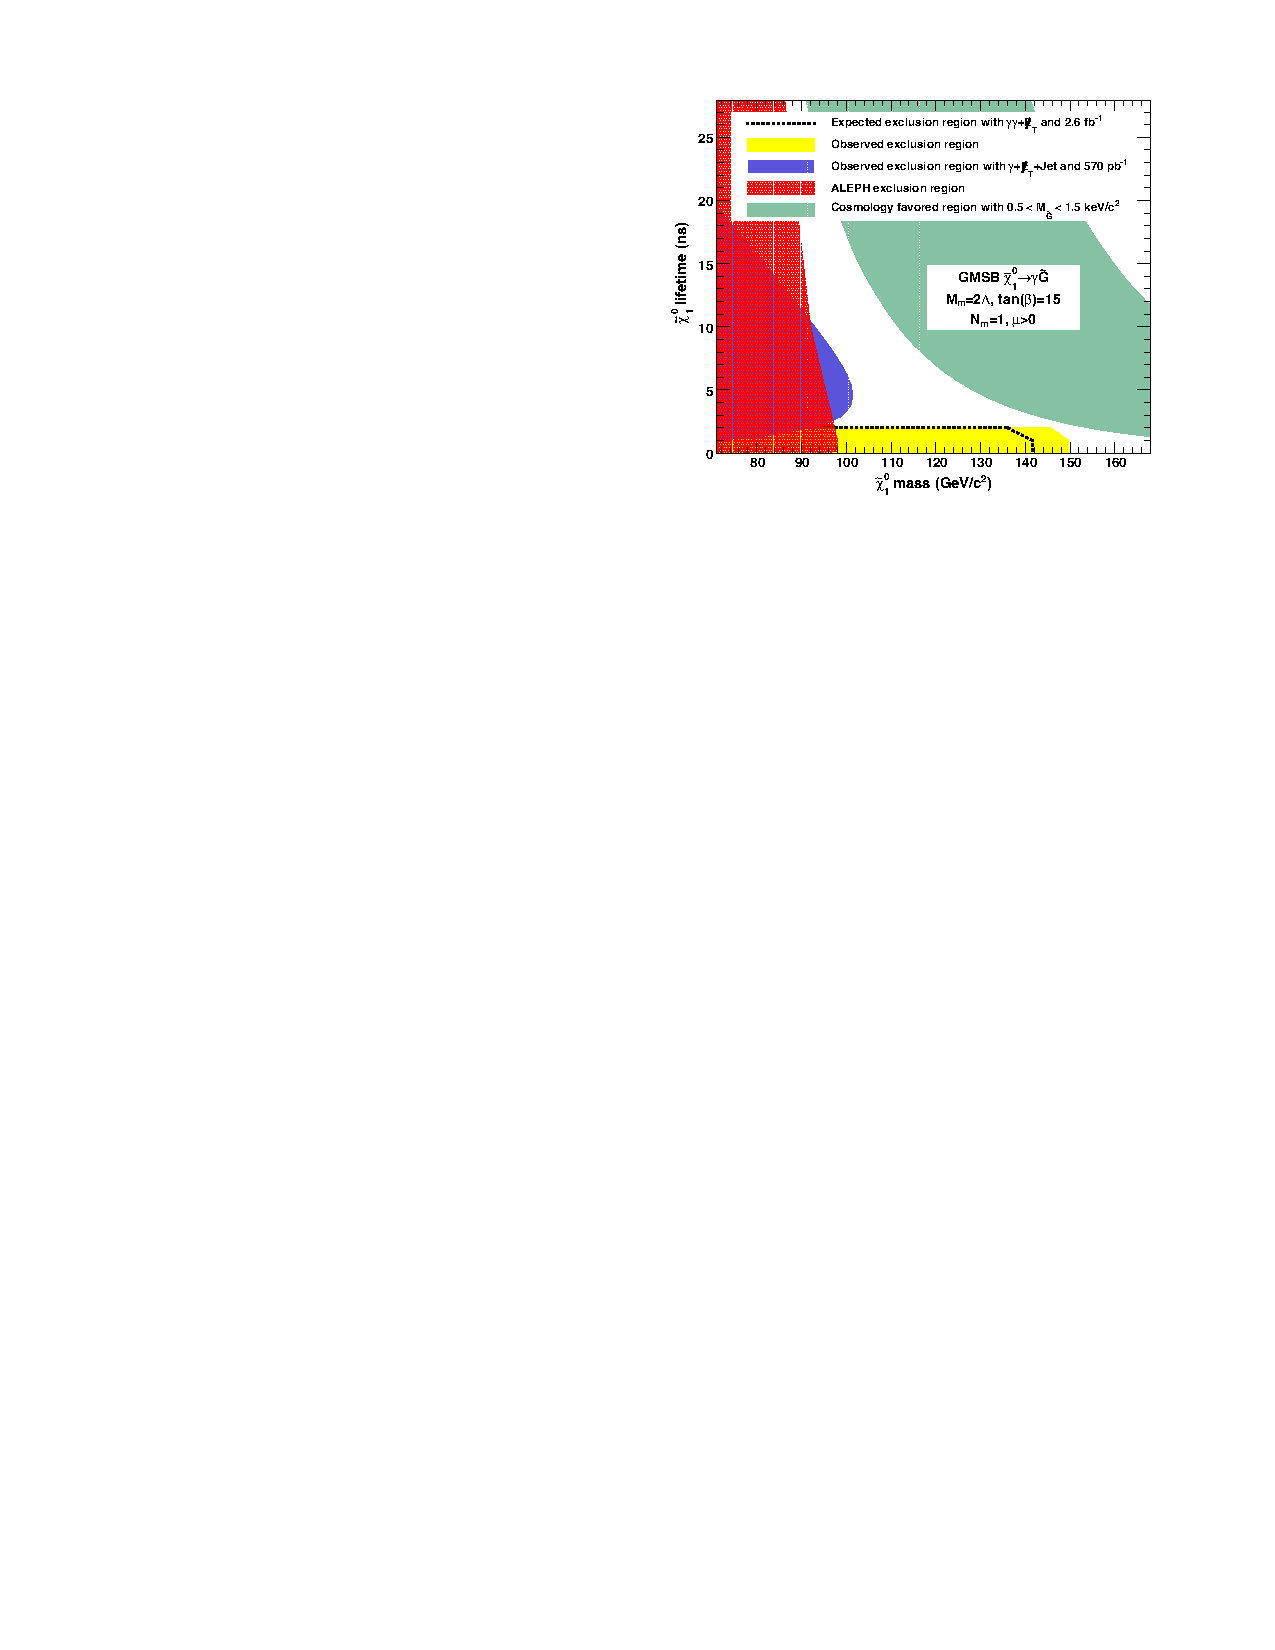
\includegraphics[scale=1.0]{CDF_lifetime_vs_mass}
	\caption{CDF exclusion contour in the $\tau_{\NLSP}$-$m_{\NLSP}$ plane, where $\tau_{\NLSP}$ is the lifetime of the neutralino.  Reprinted from ref. \cite{CDF_2010_GMSB_paper}.}
	\label{fig:CDF_lifetime_vs_mass}
\end{figure}

Finally, if the gravitino is to make up some or all of the dark matter, constraints on the form of gauge mediation must come from cosmological considerations and astronomical observations.  The gravitino in gauge mediation models is usually very light ($\mathcal{O}$(eV-MeV)) because it is proportional to the SUSY breaking scale divided by the Planck mass, and in GMSB the breaking scale is typically only of order a few hundred TeV (\cite{SUSY_primer} and Sec.~\ref{sec:Phenomenology of General Gauge Mediation}).  A light, highly relativistic dark matter particle might have been produced, for instance, in the early, radiation-dominated period of the universe \cite{Lyman_alpha_DM_limits}.  This \textit{warm dark matter} (WDM) may be responsible for all of the dark matter needed to account for galactic structure, or it may share the duties with \textit{cold dark matter} (CDM, weakly interacting particles with masses in the GeV range).  In any viable model, the predicted relic density of the dark matter species must match the observed value of $\Omega h^{2} \sim$ 0.1 \cite{WMAP}.  For many GMSB models, this measurement constrains the gravitino mass to the keV range \cite{long_lived_neutralinos_at_the_Tevatron}.  This constraint, however, does not translate into a very strong bound on the lifetime of the lightest neutralino.  Using the following equation (taken from \cite{long_lived_neutralinos_at_the_Tevatron}):

\begin{equation}
\tau_{\NLSP} \sim 130(\frac{100\mbox{ GeV}}{m_{\NLSP}})^{5}(\frac{\sqrt{\langle F\rangle}}{100\mbox{ TeV}})^{4}\mbox{ }\mu\mbox{m}
\end{equation}
%
and applying the gravitino mass constraint $\sqrt{\langle F\rangle}$ $\lesssim$ 3000 TeV (cf. the first paragraph of Sec.~\ref{sec:Phenomenology of General Gauge Mediation} with $m_{\widetilde{G}} \sim$ keV) and $m_{\NLSP}$ = 100 GeV, the upper bound on the neutralino lifetime is 100 meters.  For $\sqrt{\langle F\rangle} \sim$ 100 TeV, the neutralino lifetime is detectable on collider time scales.

Recently, a lower bound on the WDM particle mass in either pure warm or mixed warm and cold dark matter scenarios was set using observations of the Lyman-$\alpha$ forest.  For pure WDM, $m_{\mathrm{WDM}} >$ 8 keV, while for some mixed WDM-CDM scenarios, $m_{\mathrm{WDM}} >$ 1.1-1.5 keV \cite{Lyman_alpha_DM_limits, cosmo_constraints_on_GMSB}.  These bounds and others have motivated the development of more complicated gauge mediation models \cite{cosmo_constraints_on_GMSB}.  However, rather than focus on a specific GMSB model, of which there are many, the search detailed here is interpreted in a minimally model dependent way.  With this approach, the results can be applied to many competing models.  The remainder of this thesis is devoted to the experimental details of the search, analysis strategy, and presentation of the results.

\end{document}